\documentclass[12pt]{article}
\usepackage{titlesec}
\usepackage{hyperref}
\usepackage{amsmath}
\usepackage{amssymb}
\usepackage{setspace}
\usepackage{fancyhdr}
\usepackage{lastpage}
\usepackage{authblk}
\usepackage{enumitem}
\usepackage{graphicx}
\usepackage{array}
\usepackage[export]{adjustbox}
\usepackage[toc,page]{appendix}
\usepackage{listings}
\usepackage{color}
\usepackage{lipsum,graphicx,float}
\usepackage{subfig,caption}
\usepackage[raggedrightboxes]{ragged2e}
\usepackage{microtype}
\usepackage[top=1in, bottom=1in, left=1in, right=1in]{geometry}
\usepackage{longtable}
\graphicspath{ {./imgs/}{./modeling-imgs/}{./portal-imgs/}{./report-imgs/} }
\DeclareGraphicsExtensions{.png}

\definecolor{dkgreen}{rgb}{0,0.6,0}
\definecolor{gray}{rgb}{0.5,0.5,0.5}
\definecolor{mauve}{rgb}{0.58,0,0.82}
\definecolor{orange}{rgb}{0.95,0.64,0.12}

\lstset{
  frame=tb,
  language=Java,
  aboveskip=1mm,
  belowskip=1mm,
  showstringspaces=false,
  columns=flexible,
  basicstyle={\small\ttfamily},
  numbers=none,
  numberstyle=\tiny\color{gray},
  keywordstyle=\color{blue},
  commentstyle=\color{dkgreen},
  stringstyle=\color{mauve},
  breaklines=true,
  breakatwhitespace=true,
  tabsize=4
}

\doublespacing

\titleformat{\section}
{\normalfont\fontsize{14}{15}\bfseries}{\thesection}{1em}{}

\fancyhf{}
\rfoot{Page \thepage\ of \pageref{LastPage}}

\begin{document}
\begin{titlepage}
  \begin{center}
      \vspace{1cm}
      \textbf{\LARGE A Systematic Approach to Optimizing OAP Operations and Advising Processes}

      \vspace{0.5cm}
      \text{\large A Study on Systems Analysis, Design, and Software Engineering}

      \vspace{0.5cm}
      \textbf{\large Michael Maloney}

      \vspace{0.5cm}
      A Capstone Project Presented in Fulfillment\\
      of the Requirements for the Degree\\
      \textbf{\large Master of Science, Computer Science and Information Systems}\\

      \vspace{1cm}
      Department of Computer Science\\
      Congdon School of Supply Chain, Business Analytics and Information Systems\\
      University of North Carolina Wilmington\\
      2023\\
      \vspace{1cm}

      Advisory Committee\\
      \vspace{1cm}
      \begin{tabular}{ c c }
        \rule{2.5in}{0.5pt} & \rule{2.5in}{0.5pt} \\
        Dr. Judith Gebauer & Dr. Christopher Sibona \\      
      \end{tabular}

      \vspace{1.5cm}
      \rule{2.5in}{0.5pt} \\
      Dr. Ronald Vetter, Chair \\
  \end{center}
\end{titlepage}

\begin{abstract}
The OAP Operations and Advising System is a cloud-based solution designed to optimize data management for the Online Accelerated Programs (OAP) at the Cameron School of Business, University of North Carolina Wilmington. The current system, reliant on manual processes and spreadsheets, was inefficient and error-prone, hindering the OAP Operations and Advising team's ability to support the OAP programs effectively.

This paper presents the development of the OAP Operations and Advising System through a comprehensive systems analysis and design process, employing software engineering best practices. The development process involved analyzing the existing system, identifying OAP-specific requirements, and utilizing mixed-methods research, including stakeholder interviews and process observation. Quality assurance and testing, including unit testing and code coverage, ensured the system's reliability and alignment with stakeholders' expectations.

The OAP Operations and Advising System centralized data management, streamlined enrollment and advising processes, and improved the OAP team's effectiveness. Preliminary results indicated enhanced data accessibility, a better understanding of course offerings and program requirements, and a flexible, scalable system adaptable to changing needs.

The system is expected to continue supporting OAP programs and elevating the student experience. The study demonstrated the effectiveness of a systematic approach that leverages techniques and lessons from Systems Analysis and Systems Design to develop and implement a cloud-based solution for optimizing operations and advising processes.
\end{abstract}

\newpage

\tableofcontents

\newpage

\section{Introduction}
\subsection{Background and Context}
The Cameron School of Business at the University of North Carolina Wilmington offers a range of programs, including Online Accelerated Programs (OAP), designed for completion in a shorter time frame and delivered through a fully online learning environment. Due to their complexity and unique requirements, this research project focuses on OAP programs, including the Online MBA, Executive MBA, M.S. in Finance, M.S. in Business Analytics, M.S. in Supply Chain Management, and Business Foundations Certificate. The OAP programs offer flexibility and convenience, making them attractive to working professionals with full-time jobs or other personal commitments that may prevent them from attending classes on campus. The Operations and Advising team for the Online Academic Programs consists of two groups: the Operations team, which handles course scheduling, forecasting, registration, and management tasks, and the Advising team, which provides guidance and support to OAP students. These teams collaborate to ensure the seamless and efficient execution of all OAP programs.

\subsection{Problem Statement}
The growth of OAP Programs has brought about unique challenges for the OAP Operations and Advising team as they manage increased enrollment. Traditional student advising and course planning applications provided by the university do not meet the specific needs of OAP programs. As a result, the team relies on manual processes and spreadsheets to handle student advising, course forecasting, registration, and support services. However, these methods are labor-intensive and prone to errors, leading to inconsistencies and inaccuracies in data management. This hinders the team's ability to support OAP programs effectively.

Moreover, the current system requires substantial time and resources to maintain, which could be better utilized in enhancing the OAP programs and overall student experience. This paper proposes a solution to address these challenges through the development of the OAP Operations and Advising System. The system streamlines and automates necessary processes, enabling the OAP Operations and Advising team to focus on supporting the OAP programs and enhancing the student and faculty experience. This paper provides an in-depth analysis of the current challenges faced by the OAP Operations and Advising team, the development process of the new system, and its anticipated impact on managing the OAP programs at the Cameron School of Business.

\subsection{Proposed System}
The expansion of Online Academic Programs (OAP) has introduced unique challenges for the OAP Operations and Advising team in managing increased enrollment. Traditional student advising and course planning applications provided by the university are inadequate for the specific needs of OAP programs. Consequently, the team relies on manual processes and spreadsheets for student advising, course forecasting, registration, and support services. However, these labor-intensive methods are error-prone, resulting in inconsistencies and inaccuracies in data management, which impede the team's effectiveness in supporting OAP programs.

Furthermore, the current system demands significant time and resources to maintain, which could be better allocated to enhancing OAP programs and the overall student experience. This paper proposes a solution to these challenges by developing an OAP Operations and Advising System. This system streamlines and automates essential processes, allowing the OAP Operations and Advising team to concentrate on supporting the OAP programs and improving the student and faculty experience. The paper presents a comprehensive analysis of the challenges faced by the OAP Operations and Advising team, the development process of the new system, and its anticipated impact on the management of OAP programs at the Cameron School of Business.

\subsubsection{System Capabilities} 
The OAP Operations and Advising System offers a multitude of capabilities to support both the OAP Operations and Advising team and the OAP programs. Key among these capabilities is maintaining accurate, up-to-date records for each OAP student, including enrollment data, course history, and program enrollment progress tracking.

The system also streamlines the student advising process by assigning students to advisors, tracking advisor assignments, and providing advisors access to student information. Moreover, it effectively forecasts total course enrollment for each semester, considering historical enrollment numbers and maximum course capacity. This forecasting capability improves the team's planning and management of course offerings and section enrollment.

To accommodate new students with specific enrollment conditions, the system addresses limitations and requirements for program enrollment. It also offers tools for managing and updating the course catalog, such as adding new courses, removing outdated or inactive courses, and providing a centralized location for course descriptions, prerequisites, and other pertinent information.

The system aids the OAP Operations and Advising team manage their workload and tasks by tracking and reporting on enrollment and other metrics. It also serves as a centralized repository for storing and accessing essential documents and resources, such as the OAP Handbook, policies, and other relevant information. Lastly, the system acts as a communication platform among the OAP Operations and Advising team, students, and instructors, incorporating automated email and notification capabilities.

\subsubsection{Benefits and Value}
The implementation of the OAP Operations and Advising System provides significant benefits for the operations and advising teams. By optimizing workflows and automating numerous manual tasks, the system allows the team to work more efficiently, focusing on high-value activities like supporting OAP programs and improving the experience for students and faculty.

CCentralized data management offers a unified platform for recording and maintaining OAP program-related data, ensuring convenient access to current, accurate information. This approach creates a single source of truth, eliminating the need to reconcile data from various sources.

Explicitly designed for OAP programs, the system supports online course delivery, student advising, and administrative tasks, providing a customized solution rather than a generic system designed for traditional programs. This tailored design enhances data accuracy and consistency, leading to more reliable and trustworthy information while minimizing the risk of errors and omissions.

The OAP Operations and Advising System enhances transparency and provides insight into student advising and course planning processes. This enables operations and advising teams to comprehend better and optimize these processes, monitor and report key metrics and trends, and real-time access data on student enrollment, course capacity, and other relevant information.

Lastly, the system streamlines the training process for new OAP Operations and Advising team members, providing a more accessible and efficient training experience.

\subsection{Research Objectives and Questions}
This paper aims to address the following research questions, which guide the development of the OAP Operations and Advising System for the Online Accelerated Programs within the University of North Carolina's Cameron School of Business:

\begin{enumerate}[label=(\roman*)]
    \item What challenges and pain points does the OAP Operations and Advising team encounter while managing the Online Accelerated Programs at the Cameron School of Business?
    \item Which key features and requirements are needed for a system to effectively support the OAP Operations and Advising team in managing the Online Accelerated Programs?
    \item How can established software engineering methodologies and best practices be utilized in the development of the OAP Operations and Advising System?
    \item What approaches can be employed to assess the quality and effectiveness of the OAP Operations and Advising System, and what are the expected outcomes and benefits of its implementation?
\end{enumerate}

By addressing these research questions, this paper seeks to offer insights into the development process and the potential impact of the OAP Operations and Advising System on the management of the Online Accelerated Programs at the Cameron School of Business.

\section{Project Overview}
\subsection{Project Objectives}
The OAP Operations and Advising System project aims to enhance the efficiency and effectiveness of the OAP Operations and Advising team while adding value to the OAP programs. To achieve these goals, the project has established several specific objectives:

\begin{enumerate}[label=(\roman*)]
    \item \textbf{Analyze the existing system and processes:} Evaluate the current system employed by the OAP Operations and Advising team to pinpoint challenges, constraints, and unique needs and requirements of the OAP programs. This analysis offers vital insights into areas requiring enhancement, which informs the development of the new system.
    \item \textbf{Develop a comprehensive project plan:} Establish a thorough project plan that encompasses a timeline for implementing the new system, enumerating tasks and milestones, and a schedule for each project task. This plan guarantees that the project remains on track and reaches completion on time.
    \item \textbf{Design and develop a new web-based system:} Cater to the identified requirements and meet the demands of the OAP programs by designing and developing a novel web-based system. This system should handle complex data and workflow processes, offer a user-friendly interface, and ensure scalability and adaptability for future expansion.
    \item \textbf{Implement the new system and transition:} Ensure a seamless transition for the OAP Operations and Advising team to the new system by offering essential training and continuous support, encompassing regular updates and enhancements. Equipping the team with the skills to utilize the new system effectively is crucial for its success.
    \item \textbf{Improve efficiency and effectiveness:} Optimize and automate the OAP Operations and Advising team tasks to boost their efficiency and effectiveness. Provide a system that equips them with the necessary tools and resources for managing data and workflow processes, including maintaining accurate and current information on students, courses, and other pertinent data. The resulting enhancements in efficiency and effectiveness directly benefit the OAP programs.
\end{enumerate}

By pursuing these objectives, the OAP Operations and Advising System project strives to develop a resilient, user-friendly, and efficient solution that caters to the OAP programs' specific needs and bolsters the team's continued success.

\subsubsection{Success Criteria} 
The success of the OAP Operations and Advising System project is evaluated based on multiple criteria, which measure the project's attainment of its objectives and the value it provides to the OAP Operations and Advising team and the OAP programs. The following potential success criteria have been considered for the project:

\begin{enumerate}[label=(\roman*)] 
    \item \textbf{Time saved on manual tasks:} The system should significantly reduce the time and effort required by the operations and advising team to manage data and workflow processes related to the OAP programs. 
    \item \textbf{Accuracy and consistency of data:} The system should improve the accuracy and consistency of data recorded and maintained by the operations and advising team, leading to more reliable and trustworthy information. 
    \item \textbf{Efficiency and effectiveness of the OAP Operations and Advising team:} The system should enable the operations and advising team to work more efficiently and effectively, allowing them to focus on value-added activities that support the OAP programs and provide an enhanced experience for students and faculty. 
\end{enumerate}

\subsection{Project Scope and Boundaries}
The OAP Operations and Advising System project is focused on the design, development, and implementation of a web-based application that supports the activities of the OAP Operations and Advising team, including student advising and course management. The primary objectives of this project are to enhance the efficiency and effectiveness of the operations and advising team while providing value to the OAP programs through the automation of manual processes and the replacement of spreadsheet usage.

To achieve these goals within the given constraints, the project was executed in the following phases:

\begin{enumerate}[label=(\roman*)]
    \item \textbf{Project Initiation and Planning:} This phase involves defining the project scope, objectives, stakeholders, and resource requirements.
    \item \textbf{System Analysis and Design:} During this phase, stakeholders gather requirements, the existing system is thoroughly analyzed, and the new system's design is formulated.
    \item \textbf{System Development and Implementation:} This phase encompasses the actual development and testing of the new system, followed by its deployment to the production environment.
    \item \textbf{Project Closure:} This final phase involves completing all project activities, evaluating the outcomes, and delivering the final project deliverables.
\end{enumerate}

The project scope is precisely defined, centering exclusively on the development and implementation of the OAP Operations and Advising System. It does not encompass the creation or implementation of other systems or processes, nor does it involve modifications beyond the control of the OAP Operations and Advising team. Any activities or initiatives falling outside these boundaries are considered beyond the project's scope.

\subsection{Approval Process and Governance} 
The successful implementation of the OAP Operations and Advising System project requires approval from various key stakeholders to ensure its alignment with the goals and objectives of the OAP programs and the Cameron School of Business, as well as adherence to the necessary technical and security standards. The stakeholders involved in the approval process include the OAP Operations and Advising team, the Director of Graduate Student Services, the Associate Dean of Graduate Programs, and the University of North Carolina Wilmington Information Technology Services (IT) department.

The operations and advising teams actively contributed their insights and feedback regarding the project's scope and objectives, ensuring that the system addresses the specific needs and requirements of the OAP programs. The Director of Graduate Student Services and the Associate Dean of Graduate Programs thoroughly evaluated and approved the project's goals and objectives, confirming its alignment with the broader objectives of the Cameron School of Business. The IT department rigorously assessed and approved the project's technical specifications, ensuring the system adhered to stringent security and regulatory standards. The approval process was an ongoing aspect of the project, involving regular reviews and updates to ensure that the project remained on track and aligned with the evolving needs and expectations of the stakeholders.

\subsection{Explored Technologies and Alternatives} 
During the planning phase of the OAP Operations and Advising System project, thorough research was conducted to identify the most suitable technologies and tools for the development process. The research activities encompassed evaluating factors such as cost-efficiency, scalability, and availability to ensure that the selected technologies and tools align with the project's needs and requirements. Consideration was also given to the stakeholders' existing technical skills and expertise involved in the project, as well as any potential learning curves or training requirements.

The following technologies and tools were explored for the OAP Operations and Advising System project: Microsoft PowerApps, a Locally Hosted Web Application, and the Salesforce Lightning Platform. The subsequent sections provide a concise overview of each technology and tool, including a summary of the research findings and the rationale behind the final decision-making process.

\subsubsection{Microsoft PowerApps} 
The initial technology and tool explored for the OAP Operations and Advising System project was Microsoft PowerApps. Microsoft PowerApps is a low-code platform that empowers users to create custom applications without extensive coding knowledge. It is designed to be user-friendly and accessible to non-developers, offering a platform for developing and deploying straightforward applications using intuitive drag-and-drop components.

One of the notable advantages of PowerApps is its ability to integrate with various data sources, such as relational databases, SharePoint lists, and Excel spreadsheets. This flexibility in data integration proves highly advantageous for the OAP Operations and Advising System project. Furthermore, as PowerApps is available as a cloud-based service through UNCW's Office 365 subscription, it provides accessibility and feasibility.

However, it is important to acknowledge that PowerApps does have certain limitations. It is not a fully integrated development environment and lacks the advanced capabilities and flexibility required for the OAP Operations and Advising System project. The absence of robust features may impact the system's effectiveness and performance, making it challenging to meet the specific requirements of the OAP programs.

Additionally, PowerApps may not be the most scalable solution for handling significant volumes of data or supporting the complex workflow processes needed by the operations and advising team.

After a thorough evaluation, it was concluded that alternative solutions would better fulfill the capabilities, flexibility, and scalability requirements of the OAP Operations and Advising System project.

\subsubsection{Locally Hosted Web Application} 
Another option considered for the OAP Operations and Advising System was a locally hosted web application deployed on a UNCW server. The proposed development plan involved utilizing the Svelte JavaScript framework, with a local PostgreSQL server serving as the database, accessed through the web application. This locally hosted application would be accessible within the UNCW network and utilized by the operations and advising teams to record and manage data related to the OAP programs. The locally hosted solution presented cost-effectiveness and allowed OAP staff to access the application anywhere within the UNCW network. However, several limitations were identified with this option. The application would only be accessible within the UNCW network unless the operations and advising teams used a VPN.

This VPN requirement could introduce inconveniences and potential security risks for the OAP staff. After consulting with IT staff and thoroughly discussing this option's potential benefits and limitations, it was concluded that there are better alternatives to the locally hosted application for the OAP Operations and Advising System project. The primary concern against the locally hosted application environment was the potential scalability and availability issues it may present. For instance, past natural disasters like hurricanes have caused extended network outages at UNCW, rendering locally hosted databases and web applications inaccessible to UNCW staff. To mitigate such disruptions in the future, the team determined that a cloud-based solution would offer greater reliability and accessibility for the OAP Operations and Advising System.

\subsubsection{Salesforce Lightning Platform} 
The final technology and tool explored for the OAP Operations and Advising System project was the Salesforce Lightning Platform, a cloud-based Platform-as-a-Service (PaaS) offering. The Salesforce Lightning Platform encompasses a range of tools and services, including a database, development environment, and application building and deployment platform. It exhibits high scalability, can handle substantial data volumes, and support a large user base, which aligns well with the expanding and evolving needs of the OAP program. Being a cloud-based solution, the Salesforce Lightning Platform enables the OAP Operations and Advising team to access the system from any location, providing flexibility and convenience. However, the Salesforce Lightning Platform presents challenges, particularly in its subscription-based pricing model, contingent upon the number of users and data storage requirements.

After carefully considering all factors, it has been determined that the Salesforce Lightning Platform is the optimal solution for the OAP Operations and Advising System. Its robust capabilities and features align closely with the requirements of the OAP program, making it well-suited to support the effectiveness and performance of the system. The platform's scalability and accessibility ensure that the system can accommodate the needs of the operations and advising teams and effectively adapt to changes in the OAP programs.

\subsection{Selected Technology} 
The OAP Operations and Advising System project employed the Salesforce Lightning Platform to meet the specific requirements of the OAP programs and the OAP Operations and Advising team. The Salesforce Lightning Platform, a cloud-based platform, encompasses an array of tools and resources for application development and deployment. With its robust database, flow control capabilities, user interface components, and development environment, the platform is well-aligned with the needs of the OAP Operations and Advising team.

Key features and tools of the Salesforce Lightning Platform employed in the OAP Operations and Advising System project include: 

\begin{enumerate}[label=(\roman*)] 
    \item \textbf{SObject:} Provides the data model and persistence layer for the OAP Operations and Advising System. 
    \item \textbf{Apex:} Offers the OAP Operations and Advising System domain logic. 
    \item \textbf{Lightning Web Components:} Supplies the OAP Operations and Advising System presentation layer. 
    \item \textbf{Lightning Design System:} Provides the user interface design for the OAP Operations and Advising System. 
\end{enumerate}

By combining the Salesforce Lightning Platform with these specific technologies, the OAP Operations and Advising System effectively address the demands of the OAP programs and the OAP Operations and Advising team. This integration delivers a scalable and reliable system for managing data and workflow processes.

\subsection{Project Phases and Milestones} 
The OAP Operations and Advising System project followed a structured approach, consisting of several well-defined phases, each with specific tasks and objectives. These phases are outlined below:

\begin{enumerate}[label=(\roman*)] 
    \item \textbf{Project Initiation and Planning:} This phase involved the initial planning and scoping of the project, which included identifying the project's objectives, scope, and key stakeholders. It encompassed documenting the project's scope, objectives, and stakeholders. Additionally, the project plan was created, outlining the project's tasks, required resources, and timeline.
    \item \textbf{System Analysis and Design:} This phase delved into a comprehensive OAP Operations and Advising process analysis. Interviews were conducted with the OAP Operations and Advising team to gain insights into the existing processes, identify use cases, and define domain entities. Furthermore, this phase entailed defining the system's environment and architecture and identifying the system's components and their relationships. The objective of this phase was to gain a thorough understanding of the current processes, identify opportunities for improvement, and design the system to meet the needs of the OAP Operations and Advising team and its users.
    \item \textbf{System Development and Implementation:} This phase entailed the actual development and implementation of the OAP Operations and Advising System, incorporating any additional features and capabilities identified during the analysis and design phase. The aim was to ensure that the system was properly configured and set up and that the operations and advising teams had the necessary support and resources to utilize the system effectively.
    \item \textbf{Project Closure:} This final phase encompassed the completion of any remaining tasks, such as documentation and final testing, and the formal closure of the project. It also involved conducting a project review to assess the project's performance, identify areas for improvement in future projects, and verify the achievement of the project's objectives.
\end{enumerate}

\subsubsection{Project Schedule}
The OAP Operations and Advising System project commenced in March 2022 and is planned for completion in May 2023. The project team diligently monitored the progress at every stage, making necessary adjustments to maintain its trajectory and ensure its successful delivery. To visualize the project timeline, a Gantt chart has been prepared, highlighting the duration of each phase and significant milestones achieved throughout the project's duration. This comprehensive schedule management approach enabled effective project tracking, enabling the team to stay on schedule and meet project objectives within the defined timeframe.

\begin{figure}[ht]
    \centering
    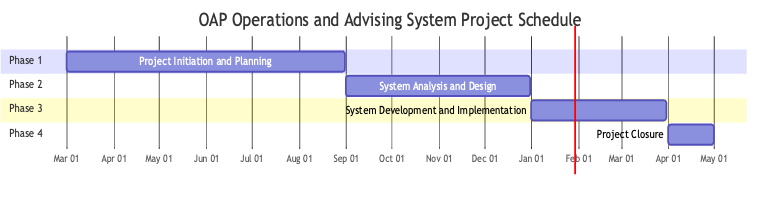
\includegraphics[width=16.5cm, height=7cm]{project-gnatt-chart}
    \caption{Project Schedule, Gantt Chart}
    \label{fig:project-schedule}
\end{figure}

\subsection{Project Deliverables}
The OAP Operations and Advising System project yielded several deliverables to support the successful implementation and use of the system. Deliverables included a fully functional system, user manual, technical documentation, and training opportunities. These deliverables provided to the OAP Operations and Advising team throughout the project's lifecycle in a phased approach to ensure the team has the necessary resources to utilize the system effectively.

\subsubsection{Functional System} 
The OAP Operations and Advising System project aims to provide the OAP Operations and Advising team with a comprehensive and fully functional system that fulfills all the requirements outlined in the project scope. To achieve this, a hybrid iterative-waterfall approach was adopted, combining the advantages of iterative development, such as continuous stakeholder feedback, with the structured delivery of a waterfall model.

Throughout the project phases, features were presented to stakeholders in multiple iterations, allowing them to provide feedback and ensure alignment with their needs and expectations. This iterative feedback process allowed for refinements and improvements to the system based on stakeholder input while maintaining the overall structure and schedule of the project.

Despite the iterative nature of feature presentation and feedback, the final system was delivered upon project completion. Prior to the final delivery, the system underwent comprehensive testing to ensure compliance with the requirements of the OAP Operations and Advising team and the OAP programs, as well as to ensure its readiness for deployment. Once the system had undergone thorough testing and validation, it was deployed to the OAP Operations and Advising team's Salesforce instance, with ongoing support provided by the OAP Operations and Advising team.

\subsubsection{User Manual and Technical Documentation}
The OAP Operations and Advising System project provided a comprehensive user manual and technical documentation to enable the OAP Operations and Advising team members to manage the OAP programs efficiently. The user manual offered clear and concise system usage instructions, including login procedures, interface navigation, student records management, and access to reports and analytics. Visual aids, such as screenshots, were also included to make it easy to understand and follow the instructions.

The technical documentation provided detailed information on the system's technical specifications, including its architecture, components, and database schema. It was presented in an easily understandable format and included visual aids such as diagrams and flowcharts to enhance clarity. This documentation served as a valuable resource for the team.

\subsubsection{Hands-on Training}
The project provided extensive training opportunities to ensure that the OAP Operations and Advising team could effectively use the OAP Operations and Advising System. This included a series of workshops conducted in person and online. The workshops covered all aspects of the system and its components, helping users understand how to use it efficiently. In addition, some team members were trained to provide support to onboard new team members and assist with the maintenance of the system.

This training was critical to the success of the OAP Operations and Advising System—providing the OAP Operations and Advising team with the necessary knowledge and skills to use the system effectively. The support-trained team members also ensured that the system was maintained and any issues were resolved promptly, further contributing to the system's success. The project's training and support were essential to implementing and using the OAP Operations and Advising System.

\section{Project Management}
\subsection{Project Management Methodology} 
The OAP Operations and Advising System project adopted a hybrid approach that integrated elements of Waterfall and Agile methodologies, incorporating the Lean practice of Kanban as a project management framework. This carefully chosen approach aimed to establish a robust foundation for the system's core components and architecture while allowing flexibility to accommodate potential changes in scope or requirements. The rationale behind this selection is detailed in the following sections.

In the initial phases of the project, a comprehensive documentation process was employed to plan the OAP Operations and Advising System using the Waterfall project management approach. This plan-driven methodology involves sequentially completing distinct phases to develop the system. The Waterfall approach ensures that the system's foundation is well-planned and sturdy, with core components and architecture meticulously configured to account for all requirements and considerations. This approach greatly benefited the project initiation and planning, system analysis and design, and early stages of system development and implementation.

As the OAP Operations and Advising System project progressed, a more Agile approach was adopted for developing additional features and capabilities. This is because the Waterfall approach, initially employed for comprehensive documentation and the establishment of core components, may need to be more adaptable to changing requirements or the incorporation of user feedback and iteration. The Waterfall approach is sequential, meaning that new requirements can only be included once the previous phase is complete, limiting the ability to incorporate feedback until the project's end. In contrast, the Agile approach prioritizes continuous delivery of valuable software and user collaboration, making it better suited for this later stage of the project. The system development and implementation phase and the system maintenance phase particularly benefited from the Agile approach. User feedback and iteration could be incorporated as the system was developed and tested in multiple iterations.

Kanban's Lean project management practice was utilized to manage the OAP Operations and Advising System project effectively. This involved creating a visual representation as a Kanban board consisting of columns representing various work stages and cards representing individual tasks. Both the Waterfall and Agile project management approaches can leverage Kanban to track the progress of work items through the system. Kanban proved advantageous for this project, as it facilitated the visualization and monitoring of task progress.

Through this hybrid approach, the OAP Operations and Advising System project ensured careful planning and configuration of core components before developing additional features and capabilities. It also provided a visual representation of the project's progression and a clear overview of its development.

\subsection{Kanban Board and Visualizing the Workflow} The Kanban board implemented for the OAP Operations and Advising System project visualizes the project's workflow and facilitates effective management of work items. It consists of several columns that represent different stages of work item progression. To ensure smooth progress and prevent bottlenecks, work-in-progress (WIP) limits have been established for specific columns, limiting the number of work items within each column to a predetermined capacity. The columns of the board are defined as follows:

\begin{enumerate}[label=(\roman*)] 
    \item \textbf{Selected for Development:} This column contains work items that have been prioritized based on their importance and urgency and are ready for development. 
    \item \textbf{In Progress:} This column represents work items currently being actively developed and tested. As a work item is initiated, it is moved to this column and remains there until it is ready for the next stage. (WIP limit: 3) 
    \item \textbf{Ready for Review:} Completed work items are placed in this column, awaiting review by the OAP Operations and Advising team. Based on the review, any necessary changes are made before advancing the work items to the next column. 
    \item \textbf{Ready for Deployment:} This column houses work items deemed ready for deployment to the production environment. 
    \item \textbf{Done:} Work items completed and approved by the OAP Operations and Advising team are placed in this column. These work items have been successfully deployed to the production environment. 
\end{enumerate}

By implementing WIP limits for each column within the OAP Operations and Advising System project, the team ensures optimal efficiency and effectiveness in completing work items, mitigating congestion or bottlenecks that may impede progress.

Regularly reviewing and updating the Kanban board is crucial to reflect work item status accurately. This can be achieved through frequent meetings with the project team to discuss progress, address any challenges, and identify workflow improvement opportunities. The Kanban board is a valuable tool for identifying bottlenecks or areas where work is not flowing efficiently, enabling the necessary adjustments to enhance productivity.

In addition to tracking and managing the project's workflow, the Kanban board can also communicate progress to stakeholders. Providing regular updates using the Kanban board informs stakeholders about work item status and overall project progress. This transparency fosters trust and confidence in the project team's ability to deliver the OAP Operations and Advising System successfully.

\subsection{Managing Project Goals and Features} 
In the OAP Operations and Advising System project, epics are crucial in tracking the progress of significant, overarching goals across multiple release cycles. These epics represent specific aspects of the system, such as developing core functionality or implementing new features. To aid in prioritization and identification, each epic is labeled with tags such as "Core," "Feature," or "Bug Fix," providing clarity on its purpose.

Work items related to a particular epic are grouped together, allowing for easy progress tracking. On the project's Kanban board, these work items are placed in a designated swim lane labeled with the epic's name. For example, all work items associated with developing the core functionality of the OAP Operations and Advising System would be grouped in the "Core" swim lane on the Kanban board. Once all the work items for an epic are completed and deployed to the production environment, the epic is closed, and the associated work items are removed from the Kanban board.

The backlog serves as a collection of all OAP Operations and Advising team feature requests that have yet to be associated with an epic. Features in the backlog are awaiting further refinement and assignment. When a feature is divided into related work items and assigned to an epic, it is removed from the backlog. If a feature request does not have an existing epic, it remains in the backlog until an appropriate epic is identified or created specifically for that feature request. The backlog serves as a repository of all feature requests, allowing the OAP Operations and Advising team to quickly identify and prioritize the features they would like to see implemented in the OAP Operations and Advising System.

\subsection{Project Management Tools}
The OAP Operations and Advising System project utilized tools to facilitate efficient and organized project management. These tools include Jira, Confluence, and Bitbucket. Each of these tools serves a specific purpose in the project management process, as described below:

\begin{enumerate}[label=(\roman*)]
    \item \textbf{Jira:} A project management platform that provides a central interface for tracking the progress of work items, including epics, user stories, and change requests. It offers a visual Kanban board, roadmap, and backlog to help the team stay organized and on track. Jira also allows team members to view the status of each work item, including which stage of completion it is in.
    \item \textbf{Confluence:} A collaboration platform that allows the team to document the project's artifacts, such as analysis documents, design documents, and meeting notes. It also serves as a central repository for project scope and requirements, including user stories, acceptance criteria, and change requests.
    \item \textbf{Github:} A version control system that stores the OAP Operations and Advising System's source code and other project artifacts, such as analysis documents, design documents, and meeting notes.
\end{enumerate}

\section{Systems Analysis}
\subsection{System Analysis Overview}
In developing the OAP Operations and Advising System, a comprehensive system analysis was undertaken to evaluate and enhance the methods and data management practices employed in managing and advising OAP graduate students. This analysis aimed to identify areas that could benefit from optimization or modification, with the ultimate goal of improving various aspects of the system. These areas included data management and storage, process efficiency, user experience, and maintainability.

The system analysis process began with rigorous data management and storage system evaluation. This examination allowed for identifying opportunities to refine data collection, storage, and retrieval mechanisms. By improving these aspects, the system aimed to ensure the accuracy and accessibility of vital information for the OAP Operations and Advising team.

Simultaneously, a thorough examination of the existing processes for managing and advising graduate students was conducted. This evaluation sought to detect any bottlenecks or inefficiencies within these processes. By identifying these areas, the project team aimed to implement process optimization strategies that would mitigate issues and improve the system's overall efficiency. Moreover, the system analysis process assessed the scalability and adaptability of the system to meet future requirements. This evaluation ensured that the system could effectively accommodate potential growth and evolving needs. Additionally, considerations were given to the ease of system maintenance and updating to guarantee its long-term viability.

By taking a holistic approach to system analysis, all critical areas for improvement were identified. This comprehensive evaluation ensured that the OAP Operations and Advising System remained effective and efficient in meeting the evolving needs of its users, contributing to the overall success of the OAP programs.

\subsubsection{System Context Diagram}
The system context diagram offers a comprehensive visual representation of the OAP Operations and Advising System, presenting an overview of its scope and interactions with external entities. Figure \ref{fig: system-context-diagram} clearly depicts the system's boundaries and the external entities that interact with it.

\begin{figure}[ht]
    \centering
    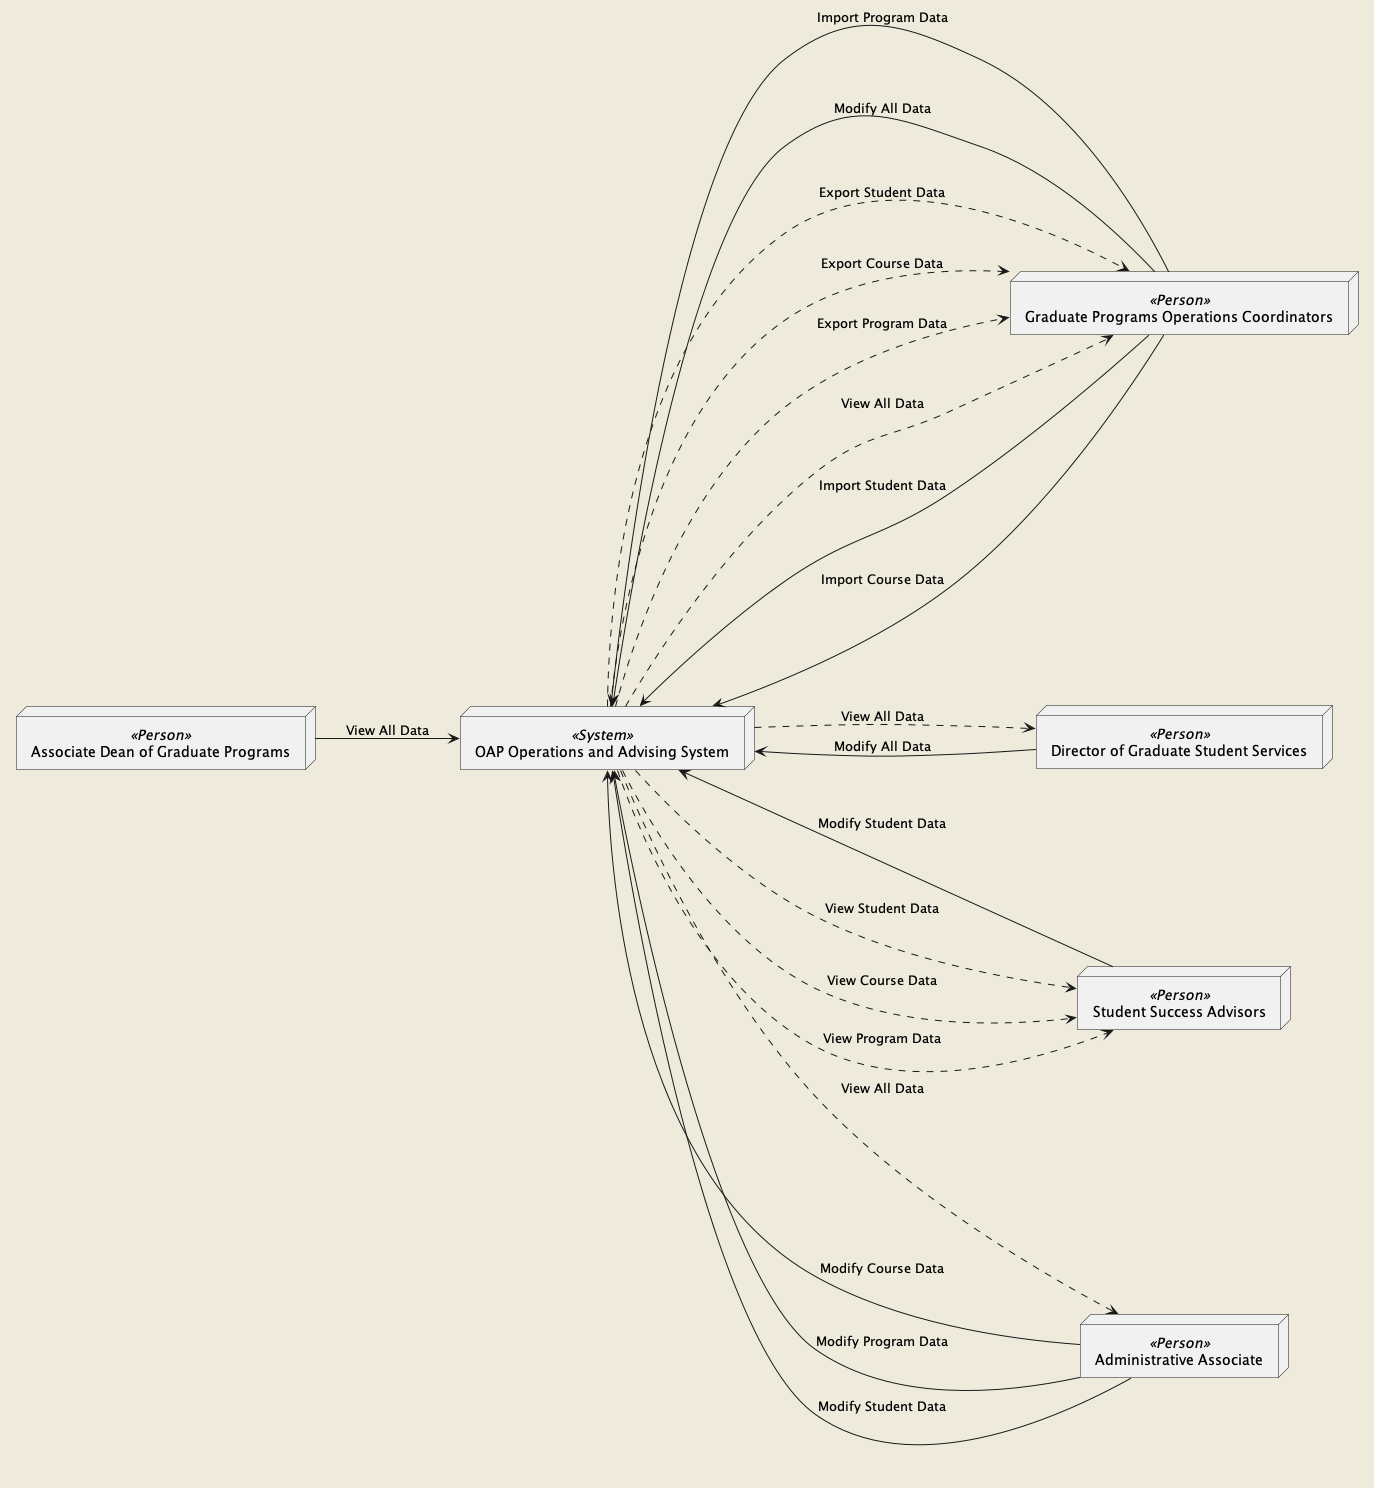
\includegraphics[width=0.9\textwidth,height=0.9\textheight,keepaspectratio]{system-context-diagram}
    \caption{System Context Diagram}
    \label{fig: system-context-diagram}
\end{figure}

\subsection{Stakeholder Analysis}
The OAP Operations and Advising System interfaces with multiple stakeholders, each having unique interactions with the system based on their specific roles and responsibilities. Each stakeholder has a unique level of involvement and specific roles and responsibilities. The following section describes each stakeholder, including their roles and responsibilities, level of involvement, and impact on the project. It is essential to understand these interactions to ensure the system effectively meets all relevant stakeholders' needs and functions.

\subsubsection{Roles and Responsibilities}
The OAP Operations and Advising System project involves several key roles and responsibilities within the Cameron School of Business graduate programs. These roles are integral to the successful management and support of the OAP programs. The following provides a detailed description of each role:

\begin{enumerate}[label=(\roman*)]
    \item \textbf{Graduate Programs Operations Coordinators} are responsible for managing the day-to-day operations of the Cameron School of Business graduate programs. This may include managing the program enrollment process, coordinating course schedules, and supporting the overall management of the graduate programs. Graduate Programs Operations Coordinators work closely with the Director of Graduate Student Services and other staff members to ensure the graduate programs run smoothly and effectively.
    \item The \textbf{Director of Graduate Student Services} is a person who is responsible for overseeing the operations and resources provided to graduate students at a university or school. This person is responsible for managing a team of student success advisors and other staff members who provide academic advising and support to students, ensuring they have the resources they need to succeed in their studies. The Director of Graduate Student Services is a pivotal member of the leadership team for graduate programs and works to ensure that the institution provides a high-quality and supportive experience for its graduate students.
    \item \textbf{Student Success Advisors} are a team of people who supports, and guides graduates students throughout their academic journey. In this role, the advisor helps students navigate course selection, monitors their progress, and offers guidance on various issues related to their education. By providing personalized support and resources, the student success advisor plays a crucial role in helping students achieve their academic goals and succeed in their program.
    \item The \textbf{Administrative Associate} is a person who is responsible for the day-to-day operations of the Graduate Student Services office. This person typically performs administrative tasks and supports the Director of Graduate Student Services and the Student Success Advisors.
    \item The \textbf{Associate Dean of Graduate Programs} manages the Cameron School of Business graduate programs. This person is responsible for ensuring that the graduate programs meet their goals and objectives and that the institution provides a high-quality experience for its graduate students. The Associate Dean of Graduate Programs works closely with the Director of Graduate Student Services and the Graduate Programs Operations Coordinators to ensure that the graduate programs run smoothly and effectively.
\end{enumerate}

\subsubsection{Level of Involvement}
The level of involvement for each role in the OAP Operations and Advising System project varies based on their responsibilities and expertise. Here is a breakdown of the level of involvement for each role:

\begin{table}[ht]
    \centering
    \caption{Stakeholder Analysis Matrix}
    \label{tab: stakeholder-analysis-matrix}
    \setlength{\leftmargini}{0.4cm}
    \begin{tabular}{| m{8.5cm} | m{7cm} |}
        \hline
        \textbf{Stakeholder} & \textbf{Stakeholder Engagement}\\
        \hline
        Graduate Programs Operations Coordinators &
        \begin{itemize}
            \item Participate in bi-weekly meetings to discuss the status of the project
            \item Provide feedback on the system design and development
            \item Provide feedback on the system testing and implementation
        \end{itemize}
        \\
        \hline
        Director of Graduate Student Services &
        \begin{itemize}
            \item Participate in bi-weekly meetings to discuss the status of the project
            \item Guide the strategic direction of the project
            \item Approve major decisions and changes
        \end{itemize}
        \\
        \hline
        Student Success Advisors &
        \begin{itemize}
            \item Provide input on system features and functionality
            \item Offer feedback on system testing and implementation
        \end{itemize}
        \\
        \hline
        Administrative Associate &
        \begin{itemize}
            \item Provide input on system features and functionality
            \item Offer feedback on system testing and implementation
        \end{itemize}
        \\
        \hline
    \end{tabular}
\end{table}

\subsection{Evaluation of Current System}
The OAP Operations and Advising team currently relies on a spreadsheet-based record-keeping system to manage and store data related to their activities, including student, course, and program records. However, this system has several limitations that impact its effectiveness and efficiency.
One significant limitation is the potential for human error in manual data entry. Manual data entry risks inaccuracies and inconsistencies, leading to incorrect or misleading information that can adversely affect the system's decision-making capabilities. For example, if a student's name requires correction during data entry, tracking their progress becomes challenging.

Another limitation is data isolation. The current system utilizes multiple spreadsheets to record and manage data related to the same entities, such as students or courses. This results in fragmented data that is difficult to consolidate and maintain consistently. Data isolation also hampers data analysis and reporting, as combining and comparing data from different spreadsheets becomes challenging. Identifying meaningful trends and patterns that can inform decision-making and improve the OAP programs is difficult.

The current system suffers from data analysis and reporting challenges. For instance, information about courses is spread across different spreadsheets, such as the Course Workbook and the Advisor Workbook, making it challenging to accurately analyze and report on a student's course schedule. The need to reference multiple spreadsheets hinders data analysis and introduces the potential for errors.

Real-time data access also needs to be improved in the current system. Team members face challenges accessing and updating data in real-time with manual data entry and separate spreadsheets. This delays decision-making and limits the team's ability to respond promptly to changing circumstances or requirements.

Furthermore, the current system lacks adequate data security measures. There are no safeguards to protect the data from unauthorized access, and no backup or version control measures are implemented. This poses risks of data loss, corruption, and unauthorized alterations.
Addressing these limitations and improving the current system's shortcomings were key objectives of the OAP Operations and Advising System project, ensuring enhanced data accuracy, efficiency, accessibility, and security.

\subsection{System Requirements}
The system requirements for the new OAP Operations and Advising System are classified into functional and non-functional categories. Functional requirements describe the desired behavior and capabilities of the system, while non-functional requirements cover quality attributes such as performance, security, and usability.

\subsubsection{Functional Requirements}
The functional requirements for the OAP Operations and Advising System are as follows:

\begin{enumerate}[label=(\roman*)]
    \item \textbf{User Management:}
    \begin{itemize}
        \item The system should support role-based user access, including roles for Graduate Programs Operations Coordinators, Student Success Advisors, and Administrative Associates.
        \item User accounts should have secure authentication and password management functionalities.
        \item The system should provide user profile management features, allowing users to update their personal information.    
    \end{itemize}
    \item \textbf{Student Management:}
    \begin{itemize}
        \item The system should allow the creation, updating, and deletion of student records.
        \item It should facilitate the assignment of advisors to students and enable the tracking of advisor-student relationships.
        \item Student records should store personal details, program enrollment, course history, and academic progress.
    \end{itemize}
    \item \textbf{Course Management:}
    \begin{itemize}
        \item The system should support creating, updating, and deleting course records.
        \item It should provide features for managing course offerings, including scheduling, session assignment, and instructor assignment.
        \item Course records should include the course name, description, prerequisites/corequisites, and credit hours.
    \end{itemize}
    \item \textbf{Program Management:}
    \begin{itemize}
        \item The system should allow the configuration and management of OAP program offerings.
        \item It should support the program requirements definition, including required courses and elective courses.
        \item Program records should store information such as the program name, description, and program-specific restrictions.
    \end{itemize}
    \item \textbf{Workflow Management:}
    \begin{itemize}
        \item The system should facilitate managing and tracking workflow processes related to student advising and course enrollments.
        \item It should support the definition and enforcement of business rules and process automation.
        \item Workflow management features should include task assignments, notifications, and progress tracking.
    \end{itemize}
    \item \textbf{Reporting and Analytics:}
    \begin{itemize}
        \item The system should provide reporting functionalities to generate predefined ad-hoc reports on student enrollment data, program statistics, and advising activities.
        \item It should support data visualization and allow users to export reports in various formats.
        \item The system should offer analytics capabilities to identify trends, patterns, and insights from the data.
    \end{itemize}
\end{enumerate}

\subsubsection{Non-Functional Requirements}
The non-functional requirements for the OAP Operations and Advising System are as follows:

\begin{enumerate}[label=(\roman*)]
    \item \textbf{Performance:}
    \begin{itemize}
        \item The system should provide fast response times and handle multiple concurrent users effectively.
        \item It should support efficient data retrieval and processing to guarantee a satisfactory user experience.
    \end{itemize}
    \item \textbf{Security:}
    \begin{itemize}
        \item The system should incorporate security measures to protect data from unauthorized access.
        \item User authentication and authorization mechanisms should be implemented to control access to system features and data.
    \end{itemize}
    \item \textbf{Usability:}
    \begin{itemize}
        \item The system should have an intuitive and user-friendly interface, requiring minimal training for users to navigate and perform tasks.
    \end{itemize}
    \item \textbf{Reliability:}
    \begin{itemize}
        \item The system should have high availability and be resistant to failures.
    \end{itemize}
    \item \textbf{Maintainability:}
    \begin{itemize}
        \item The system should be built using modular and well-documented code to facilitate future enhancements and updates.
    \end{itemize}
\end{enumerate}

\subsubsection{User Requirements Gathering} 
The OAP Operations and Advising System development involved gathering user requirements. The needs, expectations, and goals of the OAP Operations and Advising team were identified through extensive consultations and interactions with stakeholders. In order to ensure a comprehensive understanding of the requirements and their integration into the system's design, multiple interviews and discussions were conducted.

\subsubsection{Uncovering User Goals through Stakeholder Interviews} 
In order to ensure a comprehensive understanding of the needs and priorities of the OAP Operations and Advising team, a series of ongoing interviews were conducted to engage with stakeholders actively. Through this iterative process, specifications and requirements for the system's behavior and capabilities were consistently gathered and refined.

Throughout the interview phase, individual meetings were held with key personnel, including the Director of Graduate Student Services, the Associate Dean of Graduate Programs, and the Administrative Associate. These interviews yielded invaluable insights into the unique requirements of each stakeholder, enabling a thorough examination of their roles and responsibilities within the OAP Operations and Advising team.

Centered around addressing user goals and corresponding system capabilities, the design of the OAP Operations and Advising System is crucial for ensuring efficient operation and stakeholder satisfaction. These goals and capabilities encompass a diverse range of functionalities, including:

\begin{enumerate}[label=(\roman*)]
    \item Managing student enrollment: The system should track enrollment status, assist with course registration, guide and support students, and advise on academic requirements and policies.
    \item Scheduling courses, tracking enrollment, and managing waitlists: The system should store and organize student information and support administrative tasks like creating program enrollments and assigning students to advisors.
    \item Monitoring enrollment conditions and evaluating academic program requirements: The system should track students' progress toward meeting these requirements.
    \item Streamlining student management: The system should set and manage reminders and tasks, such as following up with students and generating reports on student data.
    \item Communicating with stakeholders: The system should send mass emails and facilitate the student check-up process, including creating check-ups and tracking their status.
    \item Forecasting course enrollment and planning future semesters: The system should analyze enrollment trends to inform decision-making.
    \item Integrating with external systems: The system should interact with the student information system, manage course listings and descriptions, assign instructors, and handle course override requests.
    \item Managing course availability: The system should add, cancel, or close courses based on enrollment capacity.
\end{enumerate}

\subsubsection{Use Case and User Story Development}
Use cases and user stories for the OAP Operations and Advising System have been developed based on the user goals and system capabilities identified through stakeholder interviews. These use cases and user stories offer a comprehensive view of the system's behavior and capabilities from the user's perspective, emphasizing the benefits they can derive.

For the OAP Operations and Advising System, user stories were formulated to pinpoint the specific actions and functionality required to fulfill the identified user goals and requirements. This process entailed examining the user goals and requirements gathered during stakeholder interviews and discussions. Subsequently, specific actions and functionality were identified and organized into user stories. Each user story adheres to the template: "As a(n) [actor], I want [goal], so that [benefit]."

Examples of user stories for the OAP Operations and Advising System include:
\begin{enumerate}[label=(\roman*)]
    \item As an Administrative Associate, I want to add an applied enrollment condition to a student's program enrollment, so that I can inform the Student Success Advisor of any conditions that must be met before the student can be fully enrolled.
    \item As a Student Success Advisor or Director of Graduate Student Services, I want to view a list of students assigned to me, so that I can easily access their records and provide academic advising and support.
    \item As a Graduate Programs Operations Coordinator, I want to create a template program plan of study, so that Student Success Advisors have a guide to follow when creating a customized plan of study for each student based on the program's requirements.
    \item As a Graduate Programs Operations Coordinator, I want to view and update the enrollment capacity for each course, so that I can manage course demand, ensure students can register for the courses they need to complete their program, and prevent over-enrollment in courses.
\end{enumerate}

The user stories, carefully crafted based on stakeholder input, have served as an indispensable roadmap for developing the OAP Operations and Advising System. By carefully integrating these user stories into every aspect of the system's design and functionality, the end product seamlessly caters to its stakeholders' diverse needs and expectations, ensuring a comprehensive and effective solution.


\subsubsection{Requirements Prioritization}
The requirements for the OAP Operations and Advising System have been prioritized using the MoSCoW method, which categorizes them into four groups: must-have, should-have, could-have, and won't-have. This approach enables prioritization based on the importance and urgency of each requirement, ensuring that the system is designed to meet the most critical needs first.

\begin{enumerate}[label=(\roman*)]
    \item The following requirements have been identified as must-haves:
    \begin{enumerate}
        \item Create and manage graduate programs.
        \item Create and manage student profiles.
        \item Create and manage program enrollment for students.
        \item View and update student enrollment statuses.
        \item Track and manage student academic standing.
        \item Create template program plans of study for each program.
        \item Manage semesters and course enrollment for students.
        \item View course prerequisites and corequisites in the course catalog.
        \item Track student progress towards graduation requirements.
    \end{enumerate}

    \item The following requirements have been identified as should-have:
    \begin{enumerate}
        \item Create and manage student check-ups.
        \item Manage course offerings for each semester.
        \item Update and maintain the course catalog, including course descriptions, schedules, and credit hours.
        \item Assist students with course registration and dropping courses, ensuring enrollment capacities are not exceeded.
        \item Identify and address potential issues or delays in a student's progress toward graduation.
    \end{enumerate}

    \item The following requirements have been identified as could-have:
    \begin{enumerate}
        \item Generate reports on course enrollment and demand to support informed decision-making.
        \item View reports on student progress toward meeting program requirements for targeted support.
        \item View and manage task lists for Student Success Advisors, including reminders, check-ups, and past/future due items.
        \item Schedule mass emails to faculty and students to communicate information.
        \item Customize the program plan of study for each student based on individual needs and program requirements.
    \end{enumerate}

    \item The following requirements have been identified as won't-have:
    \begin{enumerate}
        \item Direct integration with third-party systems for data exchange.
        \item Real-time notifications for student enrollment changes.
        \item Integration with the student information system.
        \item Automatic generation of degree audit reports.
    \end{enumerate}
\end{enumerate}

By prioritizing requirements in this manner, the OAP Operations and Advising System focused on delivering the most critical functionality needed to support graduate program management and student success. Additionally, valuable additional features have been considered for future implementation, depending on available time and resources.

\subsection{Domain Analysis and Modeling} 
Domain analysis and modeling is fundamental in Systems Analysis and Design, particularly for complex systems like the OAP Operations and Advising System. This process involves thoroughly examining and documenting the system's unique requirements and characteristics to create a robust solution that satisfies all stakeholders. In the OAP Operations and Advising System case, domain analysis and modeling were used to identify the system's entities and relationships, which were then used to create a domain model. This domain model is the foundation for developing more detailed diagrams and models, such as entity-relationship diagrams or data models. These models provide essential information for system design and implementation, ensuring that the final product meets stakeholder needs and aligns with domain requirements.

The process includes identifying and documenting stakeholders' requirements, business processes, and data requirements. In the OAP Operations and Advising System case, understanding the needs of various stakeholders, such as Graduate Programs Operations Coordinators and Student Success Advisors who manage and advise graduate students, was essential. A comprehensive analysis was conducted to design a system that supports their needs and the domain's business processes and data requirements.

\subsubsection{Identifying Entities and Relationships}
Identifying entities and relationships is a critical aspect of domain analysis and modeling, requiring a deep understanding of the domain. In the case of the OAP Operations and Advising System, this identification process involved multiple methods, including extensive discussions with stakeholders and domain experts, reviewing existing documentation and data sources, and analyzing relevant processes.

Through these discussions, stakeholders actively identified various entities that play crucial roles in the system, such as students, programs, courses, and semesters. By conducting a rigorous analysis of these entities, their relationships with one another were established. For example, it was determined that students are enrolled in programs consisting of concentrations and take courses offered during specific semesters. These relationships were identified through stakeholder discussions, examination of existing documentation, and review of relevant data sources.

The identified entities and relationships formed the foundation for creating a comprehensive domain model, which provides a high-level overview of the entities within the domain and illustrates their interconnections. These relationships can be classified as one-to-one, one-to-many, or many-to-many. They can be expressed using terms such as manages, associated with, enrolls in, has, teaches, advises, handles, related to, and creates.

The domain model is a guiding framework for developing more detailed diagrams and models, such as entity-relationship diagrams or data models. These refined models offer essential information that informs the system design and implementation process, ensuring that the final product meets the specific needs of stakeholders and aligns with the requirements of the domain.

\subsubsection{Entity-Relationship Diagram and Domain Class Model}
The entity-relationship diagram provides a detailed representation of the entities and their relationships within the OAP Operations and Advising System. It offers a visual depiction of the entities and their associations, showcasing the cardinality of each relationship.

Figure \ref{fig:entity_relationship_diagram} presents the Entity-Relationship Diagram for the OAP Operations and Advising System.

\begin{figure}[ht]
    \centering
    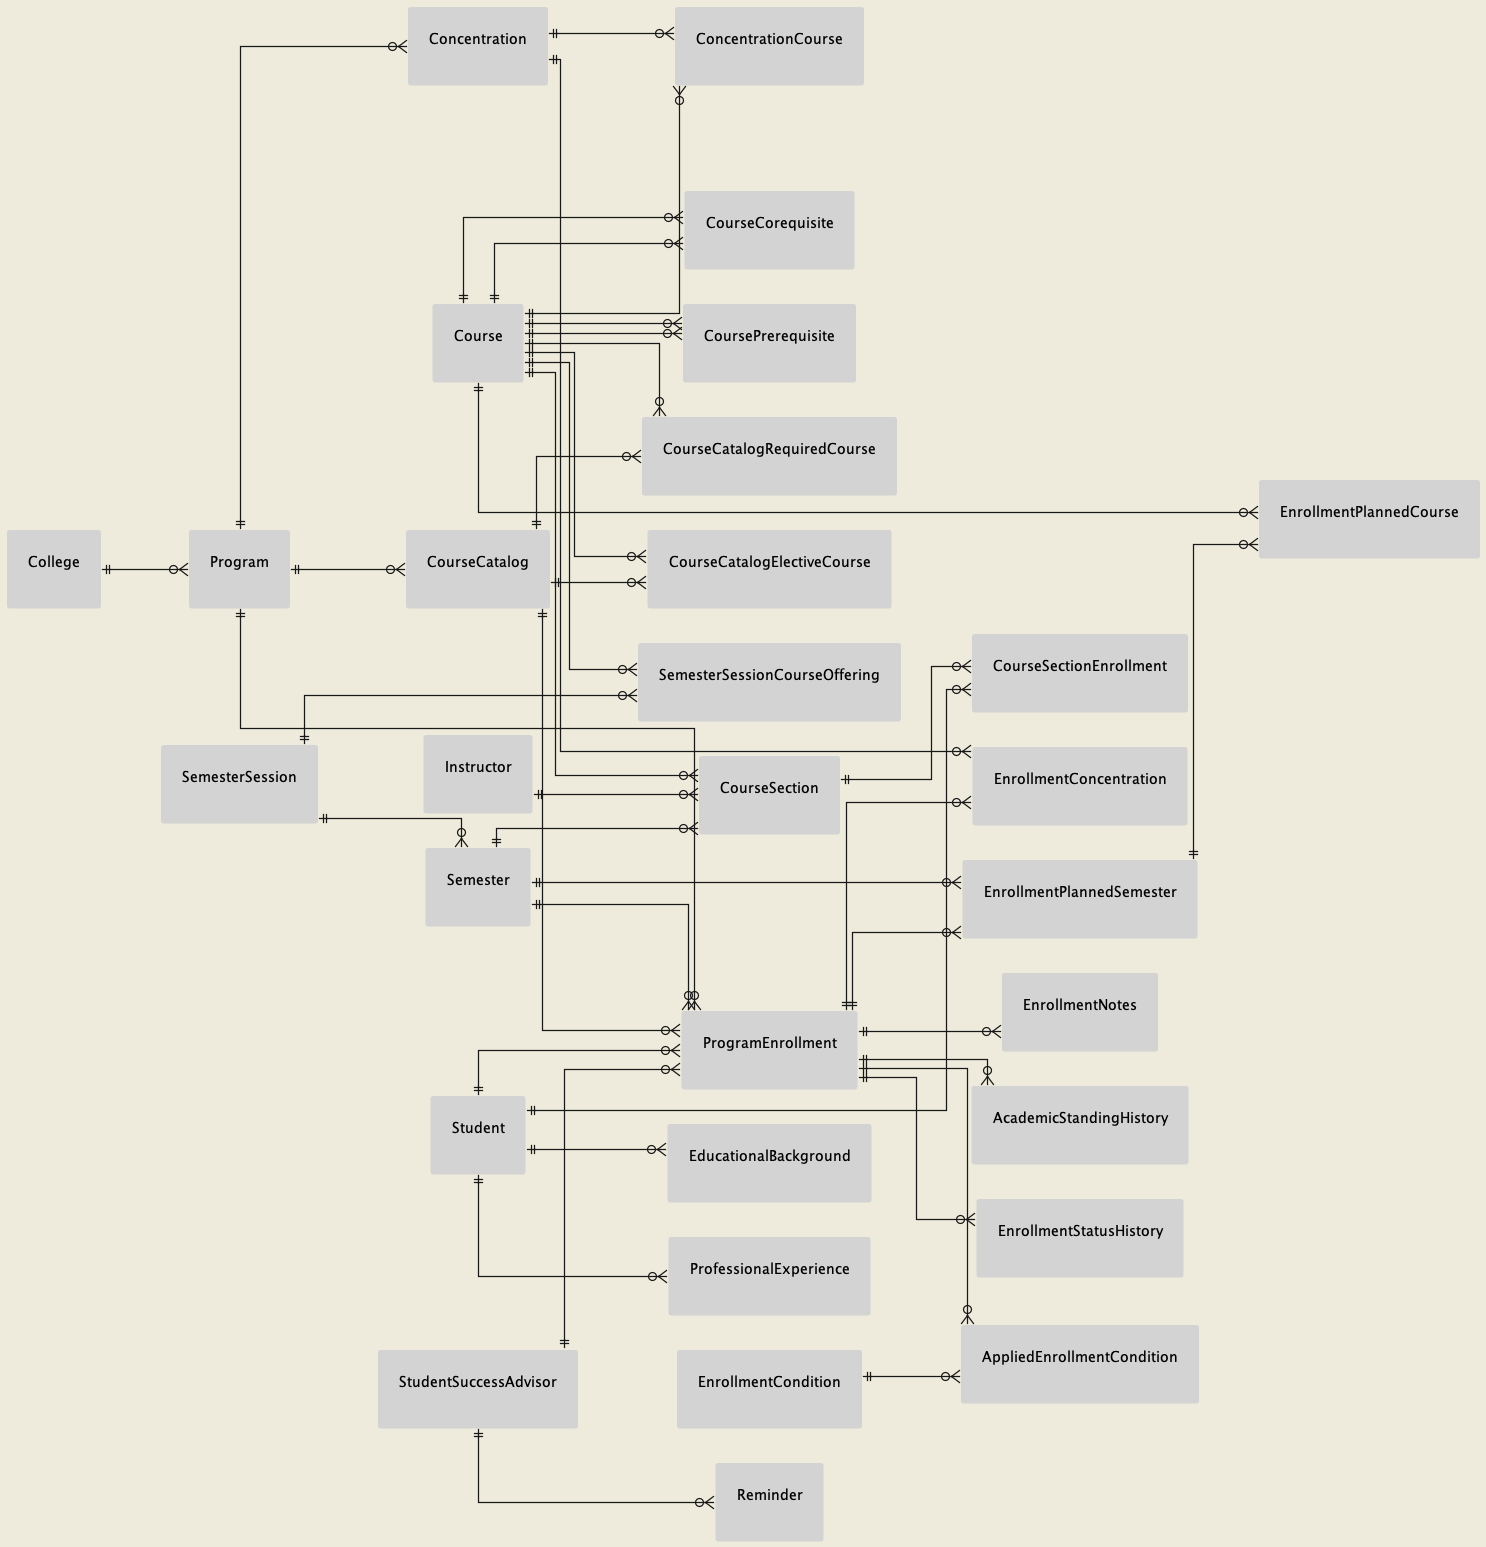
\includegraphics[width=15cm,height=15cm]{entity-relationship-diagram}
    \caption{Entity-Relationship Diagram}
    \label{fig:entity_relationship_diagram}
\end{figure}

On the other hand, the domain class model provides a comprehensive illustration of the entities and their relationships at a higher level. It highlights each entity's essential attributes and behaviors, emphasizing their interactions within the system.

Figure \ref{fig:domain_model} displays the Domain Class Model for the OAP Operations and Advising System.

\begin{figure}[ht]
    \centering
    \caption{Domain Model}
    \label{fig:domain_model}
    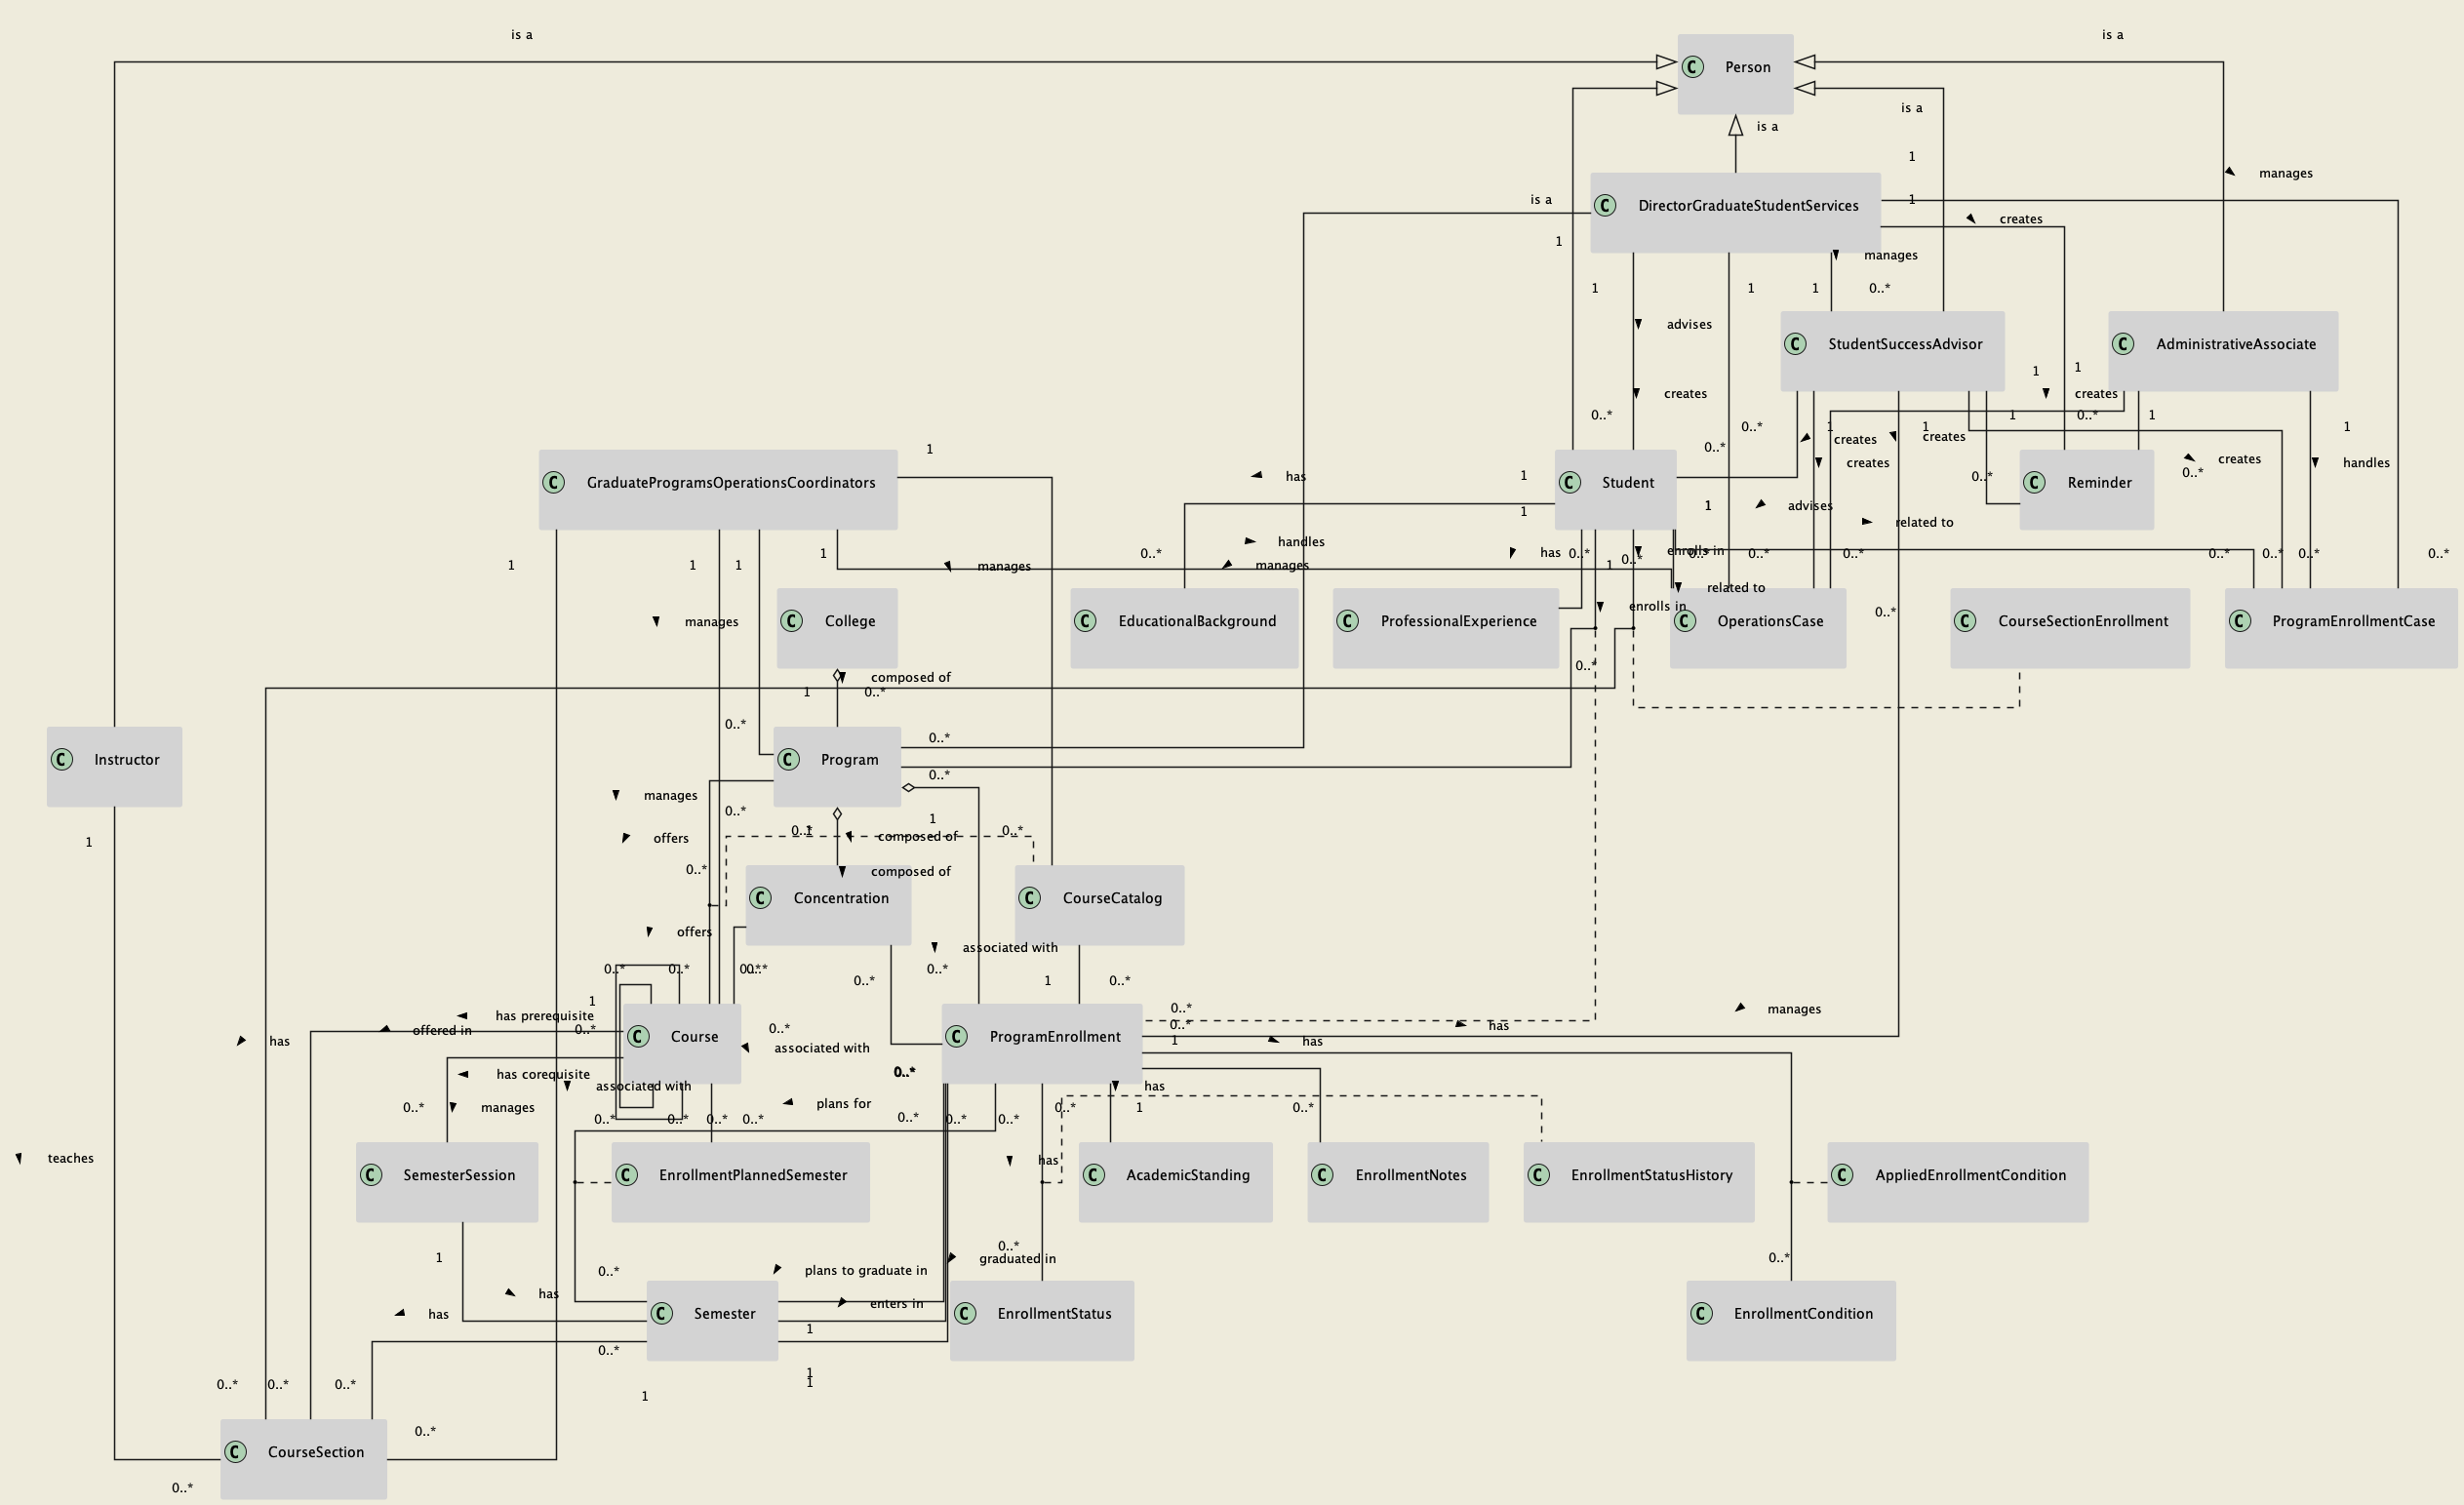
\includegraphics[width=15cm,height=15cm]{domain-class-diagram}
\end{figure}

These visual representations serve as vital tools for understanding the system's structure and organization, facilitating the project's design and implementation phases. They capture the complexities of the entities and their relationships, enabling developers and stakeholders to gain a clear and holistic view of the system's architecture.

\subsection{Use Case Analysis and Modeling}
Use case analysis and modeling is critical in system analysis and design, focusing on understanding the system's functional requirements from the users' perspective. This process involves identifying and defining the various use cases that capture the system's interactions with its actors. Use cases provide a detailed understanding of the system's behavior, specifying the actions that actors can perform and the corresponding system responses.

\subsubsection{Activity Diagrams}
Activity diagrams are visual representations that illustrate the flow of activities within a specific use case, providing a clear and intuitive view of the use case's behavior. They depict the sequence of actions performed by the system and the actors involved, capturing the steps, decisions, and conditions that govern the execution of the use case.

To better understand the behavior of the OAP Operations and Advising System, activity diagrams have been generated to represent specific use cases. These diagrams visually depict the flow of activities, showcasing the interactions between the system and the actors. The following figures present examples of activity diagrams that have been created to represent the use cases in the OAP Operations and Advising System.

Figure \ref{fig:create_student_use_case} displays the activity diagram for the "Create Student" use case, illustrating the steps in creating a new student record. The diagram showcases the interactions between the Director of Graduate Student Services and the system, capturing the validation of field values and creating a student record.

\begin{figure}[ht]
    \centering
    \caption{Create Student Use Case}
    \label{fig:create_student_use_case}
    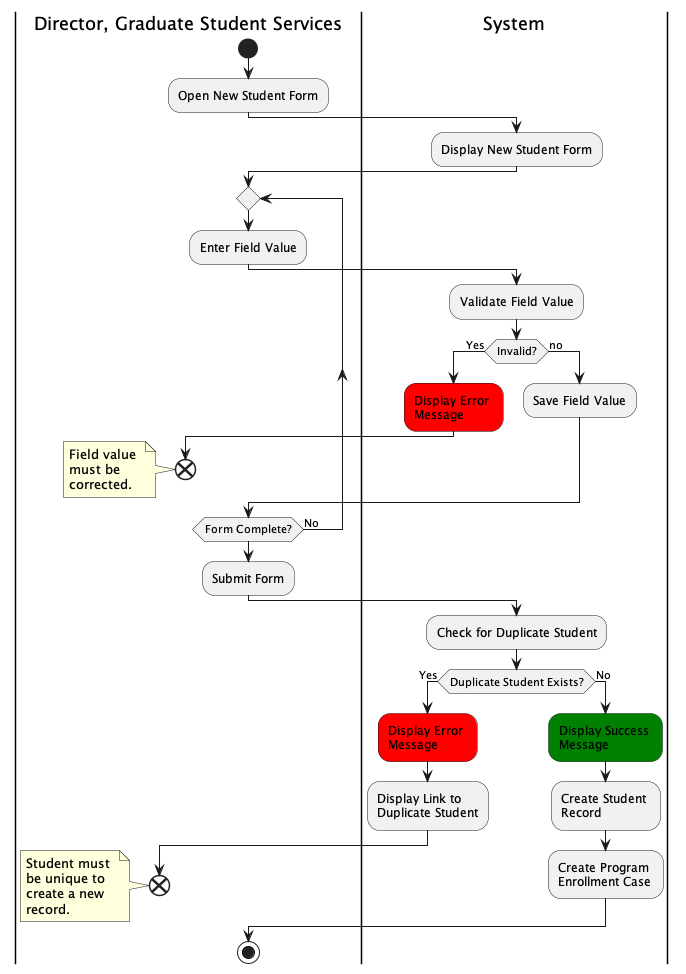
\includegraphics[width=12cm,height=12cm]{create-student}
\end{figure}

Figure \ref{fig:create_program_enrollment_use_case} displays the activity diagram for the "Create Program Enrollment" use case, illustrating the steps in creating a new program enrollment record. The diagram showcases the interactions between the director of Administrative Associate and the system, capturing the validation of field values and creating a program enrollment record.

\begin{figure}[ht]
    \centering
    \caption{Create Program Enrollment Use Case}
    \label{fig:create_program_enrollment_use_case}
    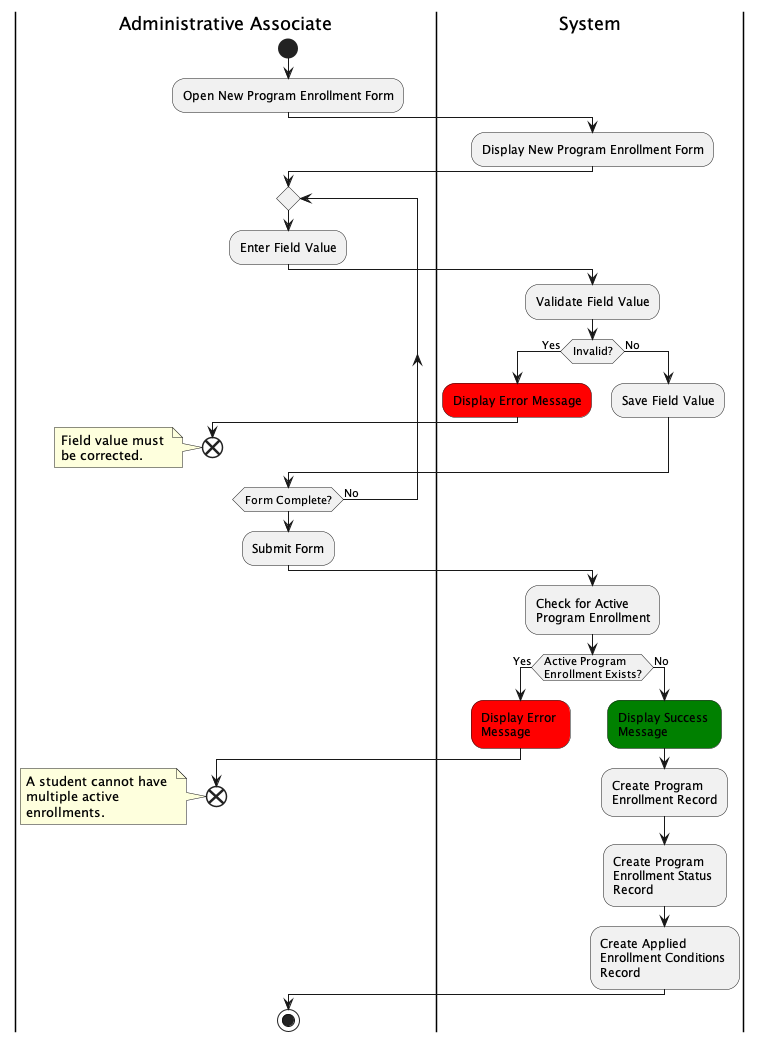
\includegraphics[width=12cm,height=12cm]{create-program-enrollment}
\end{figure}

These diagrams provide a detailed visualization of the steps and interactions involved in the use cases, offering a clear understanding of the system's behavior, and aiding in the comprehension of the system's behavior and its interactions with the users. 

\subsubsection{Use Case Descriptions}
Use case descriptions provide a comprehensive narrative of each identified use case, offering detailed insights into the interactions between actors and the system. These descriptions outline the steps required to achieve specific goals and encompass the main flow of events, alternative flows, and exceptional scenarios. By documenting the functionality of each use case, these descriptions foster a shared understanding among stakeholders and guide the design and implementation of the system.

The following use case descriptions provide examples of the identified use cases for the OAP Operations and Advising System:

\begin{longtable}[l]{|m{3.5cm}|m{12.5cm}|}
    \caption{Create Student Use Case Description} \\
    \hline
    \endfirsthead

    \hline
    \multicolumn{2}{|c|}{Continuation of Create Student Use Case Description}\\
    \endhead
    \endfoot
    \endlastfoot

    \textbf{Use Case} & Create Student\\ \hline
    \textbf{Actor} & Director Graduate Student Services\\ \hline
    \textbf{Pre-conditions} &
    \begin{itemize}
        \item The Director of Graduate Student Services has access to the system.
        \item The Director has opened the New Student Form.
    \end{itemize}\\ \hline
    \textbf{Post-conditions} &
    \begin{itemize}
        \item The student record and a program enrollment case are successfully created in the system.
    \end{itemize}\\ \hline

    \textbf{Main Flow} & 
    \begin{tabular}{m{5.25cm} | m{6.25cm}}
        Actor & System \\ \hline
        \textbf{1.} The Director opens the New Student Form. & \textbf{1.1} The system displays the New Student Form.\\ \hline
        \textbf{2.} The Director enters a field value in the New Student Form. & \textbf{2.1} The system validates the entered field value.\newline
        \textbf{2.1.1} If the field value is invalid, the system displays an error message and prompts the Director to correct the field value.\newline
        \textbf{2.1.2} If the field value is valid, the system saves the field value and proceeds to the next field.\\ \hline
        \textbf{3.} The Director submits the form. & 
        \textbf{3.1} The system checks if a duplicate student already exists.\newline
        \textbf{3.1.1} If a duplicate student exists, the system displays an error message indicating that a student with the same information already exists.\newline
        \textbf{3.1.2} If a duplicate student does not exist, the system creates a new student record and a program enrollment case.\\
    \end{tabular}\\ \hline
\end{longtable}

\begin{longtable}[l]{|m{3.5cm}|m{12.5cm}|}
    \caption{Create Program Enrollment Use Case Description} \\
    \hline
    \endfirsthead
    \hline
    \multicolumn{2}{|c|}{Continuation of Create Program Enrollment Use Case Description}\\
    \endhead
    \endfoot
    \endlastfoot

    \textbf{Use Case} & Create Program Enrollment\\ \hline
    \textbf{Actor} & Administrative Associate\\ \hline
    \textbf{Pre-conditions} &
    \begin{itemize}
        \item The Administrative Associate has access to the system.
        \item The Administrative Associate has opened the New Program Enrollment Form.
    \end{itemize}\\ \hline
    \textbf{Post-conditions} &
    \begin{itemize}
        \item The program enrollment is successfully created in the system, including the program enrollment record and applied enrollment conditions records (if applicable).
    \end{itemize}\\ \hline

    \textbf{Main Flow} & 
    \begin{tabular}{m{5.25cm} | m{6.25cm}}
        Actor & System \\ \hline
        \textbf{1.} The Administrative Associate opens the New Program Enrollment Form. & \textbf{1.1} The system displays the New Program Enrollment Form.\\ \hline
        \textbf{2.} The Administrative Associate enters a field value in the New Program Enrollment Form. & \textbf{2.1} The system validates the entered field value.\newline
        \textbf{2.1.1} If the field value is invalid, the system displays an error message and prompts the Administrative Associate to correct the field value.\newline
        \textbf{2.1.2} If the field value is valid, the system saves the field value and proceeds to the next field.\\ \hline
        \textbf{3.} The Administrative Associate submits the form. & If the form has no persisting errors, the system displays a success message and proceeds to create the program enrollment record\\
    \end{tabular}\\ \hline
\end{longtable}

\newpage

\section{Systems Design}
The systems design stage played a critical role in the overall Systems Analysis and Design process, where a comprehensive blueprint was created to implement the OAP Operations and Advising System. Building upon the requirements identified during the Systems Analysis phase, this stage focused on designing a solution that effectively addressed the needs of all stakeholders involved. The design process aimed to fulfill the previously identified requirements, facilitating efficient and effective operations and advising processes for the OAP programs.

The system design encompassed various components, each contributing to establishing a robust and adaptable foundation for the OAP Operations and Advising System. These components included system architecture, cloud computing, Salesforce infrastructure, and component decomposition. Careful consideration of these aspects ensured that the system was flexible and scalable, capable of accommodating evolving needs and requirements as the operations and advising processes of the OAP programs evolve over time.

The system architecture defined the overall structure and organization of the system, outlining its major components, their interactions, and the flow of data and information. It provided a framework that enabled effective communication and collaboration among different system elements, optimizing performance and facilitating system maintenance.

The design capitalized on cloud computing technology and leveraged the capabilities of the Salesforce infrastructure. By incorporating cloud-based resources and services, the system achieved enhanced scalability, reliability, and availability, effectively handling varying workloads and accommodating future growth while minimizing infrastructure costs and complexities. Additionally, the design utilized Salesforce's robust data management capabilities, security features, and integration options, ensuring seamless data flow and optimizing system performance for the OAP Operations and Advising System.

Component decomposition is a crucial step in system analysis and design, aimed at breaking down the OAP Operations and Advising System into smaller, manageable components. Each component is assigned specific functionalities, enabling a modular design approach that facilitates easier development, maintenance, and updates. Composing the system into cohesive components enhances system flexibility, as it allows for the decoupling of components. This decoupling promotes more efficient problem-solving and troubleshooting, as issues can be isolated and addressed without impacting the entire system.

By incorporating these design considerations, the OAP Operations and Advising System was developed with a solid foundation to support efficient operations and advising processes, as well as facilitate future growth and evolution. This design approach ensured a reliable and scalable solution for the OAP programs and their stakeholders, providing a robust platform for effective operations and advising throughout the system's lifecycle.

\subsection{System Architecture}
The OAP Operations and Advising System utilizes the Salesforce Lightning Platform developed to observe an event-driven and microservices architecture. This type of architecture supports a flexible and scalable system foundation that can adapt to an organization's changing needs and requirements as its operations and advising processes evolve. To implement its core functionality and manage the system's data, logic, and user interface, the system combines SObjects, Apex Classes, Apex Triggers, SOQL, SOSL Queries, Lightning Web Components, and the Lightning Design System.

\subsubsection{Architectural Patterns}
The OAP Operations and Advising System utilizes event-driven and microservices architectures to establish a flexible and scalable foundation. Leveraging the Salesforce Lightning Platform, built upon a microservices architecture, the system supports the development of customized applications. The event-driven aspect enables automated responses to events and changes, empowering operations and advising teams to automate tasks and execute custom actions based on data changes. The microservices architecture facilitates the creation of loosely coupled services that can be developed, deployed, and maintained independently, providing long-term flexibility and scalability. The OAP Operations and Advising System can readily adapt to evolving needs and requirements by embracing the event-driven and microservices architecture.

\textit{Event-driven architecture} is a design pattern that facilitates communication between system components through generating and consuming events. This architecture promotes loose coupling and asynchronous communication using messages, resulting in a highly scalable system that can handle failures gracefully. Each component operates independently and manages failures without impacting the overall system.

\textit{Microservices architecture} is a design pattern that decomposes an application into smaller, independent services. This approach enables high scalability and fault tolerance, as services can be developed and deployed independently and handle failures without affecting the entire system.

In the OAP Operations and Advising System, the combination of event-driven and microservices architectures ensures high scalability and resilience. The system is comprised of independent services that communicate asynchronously, providing flexibility and adaptability. Services can be developed and deployed independently and can handle failures without disrupting the entire system.

The event-driven architecture in the OAP Operations and Advising System manages and triggers actions in response to events. This approach centers around events guiding the system's behavior rather than direct requests. The Salesforce Lightning Platform supports this architecture with tools like Apex Triggers, which allow developers to define custom behavior triggered by specific events within the system. The corresponding Apex Trigger is activated when a CRUD operation (Create, Read, Update, Delete) is performed on an SObject record. It publishes the new state of the record and the old state (if applicable) to an invoked Apex Class, enabling the execution of custom logic and actions tailored to the event.

\subsection{Component Decomposition}
The OAP Operations and Advising System will use various components provided by the Salesforce Lightning Platform to support the tasks and functions stakeholders require. These components include SObjects for data storage and management, Apex Classes for custom logic and business rules, Apex Triggers for automating tasks and processes based on specific events or conditions, and SOQL and SOSL Queries for retrieving data from the system's database. The system will also utilize Lightning Web Components to construct interactive and user-friendly interfaces and the Lightning Design System to ensure a consistent and visually appealing design across all system components. These components will work together to create a flexible and scalable foundation for the OAP Operations and Advising System, allowing it to adapt to changing needs and requirements as its operations and advising processes evolve.

\subsubsection{SObjects}
Salesforce Objects, or SObjects, are fundamental to the OAP Operations and Advising System. They represent various domain entities in the system, such as students, courses, programs, and other data. SObjects are similar to database tables in that they store and manage data within the system. Each SObject has a corresponding record type that defines its structure and properties, including the fields and data types of the SObject.

SObjects can be queried and manipulated using the Salesforce Object Query Language (SOQL) and Salesforce Object Search Language (SOSL), query languages used to search and retrieve data from Salesforce objects. They can also be related through parent-child, lookup, and master-detail relationships. This is similar to how database tables can be related to each other through foreign keys.

\subsubsection{Apex Classes}
Apex Classes are custom classes written in Apex, a programming language used on the Salesforce platform. These classes can be called from Apex Triggers, other Apex Classes, and front-end Lightning Web Components to execute their logic. In the OAP Operations and Advising System, Apex Classes will implement custom functionality, including domain logic and data validation.

Apex is an object-oriented language similar to popular programming languages like Java and C\#. In the OAP Operations and Advising System, Apex Classes will be used to create custom methods to perform custom operations and actions within the system. These classes provide a flexible way to add custom functionality to the system, helping it better meet the needs and goals of stakeholders.

\subsubsection{Apex Triggers}
Apex Triggers are executed in response to a CRUD (create, read, update, delete) operation performed on an SObject. These triggers provide access to several context variables that hold information about the trigger event, including the type of operation performed, the number of records affected, and the old and new states of the record.

Apex Triggers have access to the following context variables that hold information about the trigger event:
\begin{table}[ht]
    \begin{tabular}{|l|p{13cm}|}
        \hline
        \textbf{Variable} & \textbf{Description} \\ \hline
        \textit{operation type} & This variable holds the type of operation performed on the record (create, update, delete) \\ \hline
        \textit{size} & This variable holds the number of records the operation affects. In cases where multiple records are affected, this variable will contain the total number of records affected. \\ \hline
        \textit{new} & This variable holds the new state of the record as a list of fields. \\ \hline
        \textit{old} & This variable holds the old state of the record as a list of fields. \\ \hline
        \textit{newMap} & This variable holds the new state of the record as a map of fields, with the record ID as the key. \\ \hline
        \textit{oldMap} & This variable holds the old state of the record as a map of fields, with the record ID as the key. \\ \hline
    \end{tabular}
\end{table}

Apex Triggers can be classified into two main types: "before" triggers and "after" triggers.

Before triggers are executed before the data is saved to the server, allowing for tasks like data validation, field updates, and email notifications. For instance, a before trigger can be utilized to ensure a picklist field is set to a specific value based on certain conditions. Additionally, if a developer intends to send an email to the user after creating or updating a particular record, a before trigger can initiate this action.

On the other hand, after triggers are executed after the data has been saved to the server. They are employed to perform actions like updating parent or related records and creating additional related records. For instance, an after trigger can be employed when a developer wishes to create a task associated with an edited opportunity. Another scenario where an after trigger may be applied is when a developer aims to modify the value of a lookup field on a related record based on the edited opportunity.

The graph below illustrates the relationship between Apex Triggers and SObjects. It also shows the different types of triggers and the context variables they have access.

\begin{figure}[ht]
    \centering
    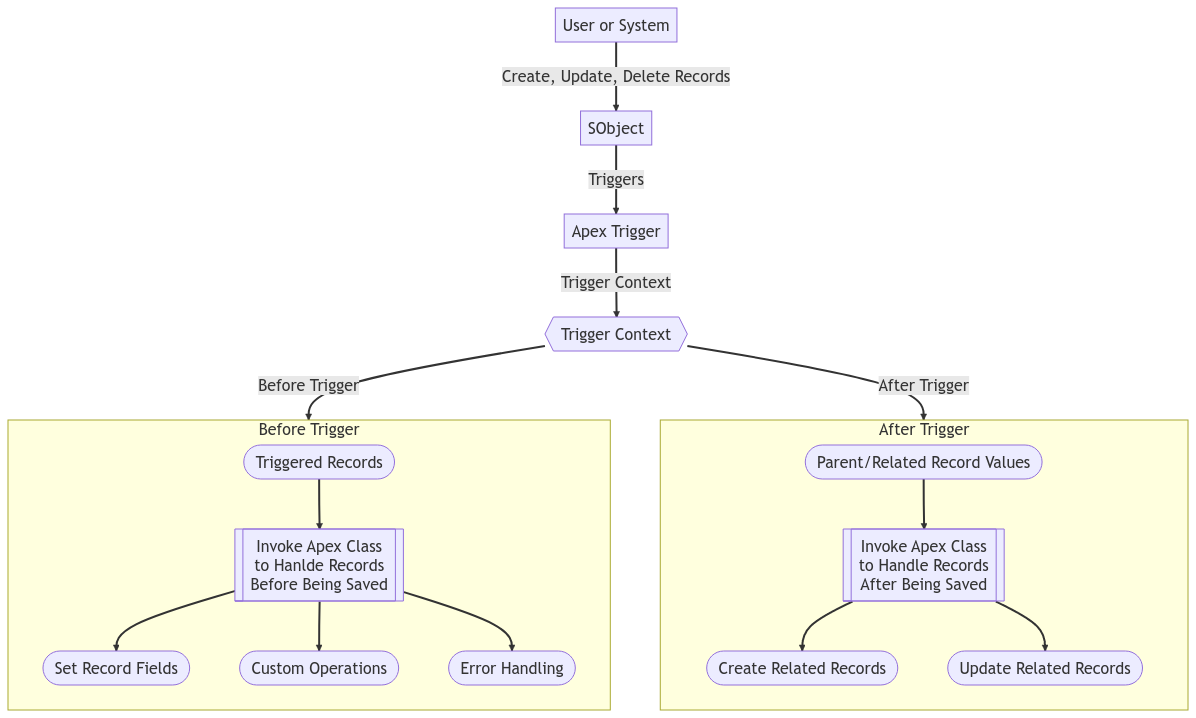
\includegraphics[max size={\textwidth}{\textheight}]{apex-trigger}
    \caption{Apex Triggers}
\end{figure}

\newpage

\subsubsection{SOQL and SOSL}
SOQL (Salesforce Object Query Language) and SOSL (Salesforce Object Search Language) are query languages used to search and retrieve data from Salesforce objects. SOQL is used to search and retrieve data from a single object, while SOSL is used to search and retrieve data from multiple objects. Both languages are supported by the Salesforce Lightning Platform and are used within the Apex programming language to search and retrieve data from Salesforce objects.

In the OAP Operations and Advising System, SOQL and SOSL will retrieve data from relevant objects and make it available to Apex code and Lightning Web Components for further processing and presentation to users. By using SOQL and SOSL, the OAP Operations and Advising System can effectively retrieve and utilize data to support its various tasks and functions.

\subsubsection{Lightning Web Components}
Lightning Web Components (LWC) is a modern programming model for building web applications on the Salesforce platform. They are built on open standards such as HTML, JavaScript, and CSS and provide a lightweight, fast, and easy-to-use framework for building custom user interfaces and applications.

In the OAP Operations and Advising System, LWCs will be used to build custom user interfaces and applications, providing a powerful and flexible way to create a consistent and efficient user experience. They are reusable components that can be easily shared and reused throughout the system, allowing for a consistent and efficient development process. LWCs are also designed to be optimized for performance, with a minimal footprint and fast rendering times, which will help ensure that the system is responsive and efficient.

\subsubsection{Lightning Design System}
The Lightning Design System is a collection of design guidelines, patterns, and components that can create consistent and visually appealing user interfaces for applications on the Salesforce Lightning Platform. It includes a set of design tokens that define the look and feel of the interface, such as colors, typography, and spacing, as well as a library of reusable UI components, such as buttons, forms, and data tables, that can be used to build out the user interface of the OAP Operations and Advising System.

The Lightning Design System helps ensure the system's user interface is cohesive and follows best practices in user experience design. It also makes it easier to maintain and update the interface over time, as changes to the design system will be automatically reflected in the user interface. By utilizing the Lightning Design System, the OAP Operations and Advising System can create a visually appealing and consistent user interface that is easy to use and maintain.

\subsection{Access Control and Security}
Access control and security measures are crucial for the OAP Operations and Advising System, considering the involvement of multiple users with varying roles and permissions. Several security measures will be implemented to ensure a secure system environment and restrict unauthorized access, including user roles, permissions, and record-level security.

\subsubsection{User Roles and Permissions}
Role-based access controls (RBAC) will be implemented to enhance security by limiting access to specific data and system features based on user roles. This approach ensures that users only have access to the data and functionalities necessary for their job responsibilities, mitigating the risk of unauthorized access to sensitive information.

The OAP Operations and Advising System will incorporate four primary user roles, each with distinct access levels and permissions to maintain data security and uphold system integrity:

\begin{enumerate}[label=(\roman*)] 
    \item \textbf{OAP Operations User} - This user role is designated for users primarily responsible for performing operations tasks within the system. Users with this role will have complete access to all system data, including import/export capabilities, modification, and viewing. Additionally, they can utilize the system's reporting features to generate reports and access dashboards for comprehensive data analysis. 
    \item \textbf{OAP Advising User} - Users assigned this role will primarily engage in advising tasks within the OAP Operations and Advising System. They will have read and write access to student records and related information, such as planned courses and semesters. However, their access will be limited to read-only for program and course data. 
    \item \textbf{OAP Director User} - This user role encompasses users responsible for both advising and operations tasks. Users with this role will possess read and write access to all system objects, enabling them to create, edit, and modify records as necessary. 
    \item \textbf{OAP Administrative Associate User} - Users assigned this role will primarily handle administrative tasks within the OAP Operations and Advising System. Their access will entail read and write permissions for specific system objects, enabling them to create, edit, and modify relevant records as required. 
\end{enumerate}

By defining these user roles, the OAP Operations and Advising System ensures that each user is granted appropriate access and permissions in accordance with their responsibilities. This framework guarantees data security and maintains the system's integrity by ensuring users can perform their designated tasks without unauthorized access to sensitive information.

\subsection{User Interface Design} 
The user interface design of the OAP Operations and Advising System prioritizes usability and efficiency, enabling stakeholders to perform their tasks effectively. To achieve this, a comprehensive prototyping process was employed, involving creating and testing various design concepts. Low-fidelity wireframes were initially developed to explore different layout and navigation options, and these concepts were refined through iterative prototyping and stakeholder testing.

\subsubsection{User Interface Components and Layouts} 
The user interface of the OAP Operations and Advising System was built using the Lightning Web Components framework, which leverages modern web development technologies and REST APIs. This framework ensures a scalable and responsive user experience capable of handling many users and transactions. The user interface is designed to provide meaningful feedback and efficient error handling, facilitating quick resolution of any issues that may arise.

\subsubsection{Operations Console and Portal Overview} 
The OAP Operations and Advising System offers two main presentation views: the Operations Console and the Advising and Administration Portal. The Operations Console, a web-based experience hosted on the Salesforce Lightning Platform, provides comprehensive tools and resources for program and course management, case management, and reports and analytics. On the other hand, the Advising and Administration Portal caters to the needs of Student Success Advisors, Administrative Associates, and Directors of Graduate Student Services. This portal enables them to efficiently manage and support student academic programs, track student progress, manage program enrollment and requirements, and engage with students through check-ups and case management.

\subsubsection{Navigation and User Interface Components}
The user interface incorporates various components such as navigation bars, home pages, forms, and layouts to accommodate different user roles and tasks. The navigation bar offers convenient access to frequently used features and allows users to navigate seamlessly between different system pages. The home page is tailored to each user role, providing relevant information and task summaries, including upcoming deadlines, assigned tasks, and notifications. Forms and layouts are thoughtfully designed to facilitate the collection and presentation of data, ensuring that users can enter and review information in a structured and user-friendly manner.

\section{Software Engineering and Implementation} 
\subsection{Design Patterns and Principles} 
The development of the OAP Operations and Advising System prioritized the integration of design patterns to enhance the codebase's organization, structure, and maintainability. This intentional focus on design patterns was pivotal in establishing a robust software architecture capable of adapting and evolving alongside changing requirements.

Design patterns are categorized into three primary groups: creational, structural, and behavioral patterns. Creational patterns primarily address object instantiation, while structural patterns focus on class and object composition. Behavioral patterns, on the other hand, deal with interactions between objects.

In developing the OAP Operations and Advising System, various design patterns have been seamlessly incorporated to tackle specific challenges and fulfill the system's requirements. These patterns include the Facade pattern (a structural pattern), Adapter pattern (a structural pattern), Template Method pattern (a behavioral pattern), Command pattern (a behavioral pattern), and Builder pattern (a creational pattern). Each pattern was carefully selected based on its suitability for resolving particular issues and enhancing the overall system design.

The OAP Operations and Advising System has achieved a well-structured and maintainable codebase by incorporating these design patterns into the development process. This ensures that the system can readily accommodate future modifications and extensions as the needs of the OAP programs evolve.

The following sections will delve into the specific design patterns and principles employed during the development of the OAP Operations and Advising System. Through this exploration, we aim to comprehensively understand how these patterns contribute to the system's overall architecture and functionality. This analysis will shed light on the significance of these patterns in facilitating the system's design and implementation, highlighting their crucial role in ensuring a robust and adaptable OAP Operations and Advising System.

\subsubsection{Facade}
The Facade pattern is a structural design pattern that simplifies the interaction with a complex subsystem or set of related interfaces \cite{b1}. Its primary objective is to provide a higher-level interface that abstracts away the underlying complexity of the subsystem. In the OAP Operations and Advising System, the Facade pattern is employed in the \textit{JsonSObjectConverter} class to simplify converting JSON data into SObjects.

The \textit{JsonSObjectConverter} class acts as a facade, encapsulating the complex conversion process and providing a straightforward interface for clients to convert JSON data into SObjects. By utilizing the Facade pattern, clients can perform the conversion without understanding the intricate details of the underlying implementation.

Here is an example code snippet that demonstrates the implementation of the Facade pattern in the \textit{JsonSObjectConverter} class:

\begin{lstlisting}
public class JsonSObjectConverter {
    // ...Constructor and other class variables...
    
    // ...Public method to convert JSON data into an SObject...
    public SObject toSObject() {
        JsonAdapter.SObjectAdapter sObjectAdapter = new JsonAdapter.SObjectAdapter();
        Map<String, Object> sObjectData = this.adpatJsonData(sObjectAdapter.adapt(this.sObjectJsonData));
        SObjectBuilder builder = new SObjectBuilder(
            MetadataRepository.getSObjectMetadata(this.sObjectName)
        );
        builder.setAllFields(sObjectData);
        return builder.getSObject();
    }

    // ...Public method to convert JSON data into a list of SObjects...
    public List<SObject> toSObjectList() {
        JsonAdapter.SObjectListAdapter sObjectListAdapter = new JsonAdapter.SObjectListAdapter();
        List<Map<String, Object>> sObjectDataList = sObjectListAdapter.adapt(this.sObjectJsonData);
        List<SObject> sObjectList = new List<SObject>();

        for (Map<String, Object> sObjectData : sObjectDataList) {
            JsonAdapter.SObjectListAdapter sObjectAdapter = new JsonAdapter.SObjectListAdapter();
            SObjectBuilder builder = new SObjectBuilder(
                MetadataRepository.getSObjectMetadata(this.sObjectName)
            );
            builder.setAllFields(sObjectData);
            sObjectList.add(builder.getSObject());
        }

        return sObjectList;
    }

    // Private method to adapt JSON data
    private Map<String, Object> adpatJsonData(Map<String, Object> sObjectData) {
        // ...Adapting JSON data using data type adapters...
        return sObjectData;
    }
}

public class JsonAdapter {
    // ...Adapters for different JSON conversions...
}

public class SObjectBuilder {
    // ...Builder for constructing SObjects...
}

public class MetadataRepository {
    // ...Repository for obtaining metadata...
}    
\end{lstlisting}

The \textit{JsonSObjectConverter} class acts as a facade, providing a simplified interface for clients to convert JSON data into SObjects. It utilizes the \textit{JsonAdapter} class to adapt the JSON data and the \textit{SObjectBuilder} class to construct the SObjects. The necessary metadata for the conversion process is obtained from the \textit{MetadataRepository} class.

The \textit{toSObject()} method converts JSON data into a single SObject. It uses the \textit{JsonAdapter.SObjectAdapter} class to adapt the JSON data into a \textit{Map<String, Object>}. The \textit{SObjectBuilder} class is then used to construct the SObject based on the adapted data.

Similarly, the \textit{toSObjectList()} method converts JSON data into a list of SObjects. It utilizes the \textit{JsonAdapter.SObjectListAdapter} class to adapt the JSON data into a list of \textit{Map<String, Object>}. Iterating over the list, the \textit{SObjectBuilder} class constructs individual SObjects based on each adapted data item and adds them to the \textit{sObjectList}.

By encapsulating the conversion process and exposing only the necessary methods, the \textit{JsonSObjectConverter} class simplifies the subsystem usage. Clients can convert JSON data into SObjects by invoking the appropriate method without needing to understand the internal implementation details.

This implementation of the Facade pattern enhances code readability, maintainability, and reusability. It separates the conversion logic, reducing dependencies and making the code easier to understand and modify. Clients can focus on the higher-level functionality without worrying about the intricacies of the JSON-to-SObject conversion.

\subsubsection{Template Method}
The Template Method pattern is a behavioral design pattern that provides a template for a specific algorithm while allowing subclasses to define their implementation details \cite{b1}. It promotes better separation of concerns and helps manage complex code bases by defining a set of methods that subclasses can implement to customize the algorithm's behavior.

The \textit{TriggerManager} class utilizes the Template Method pattern in the provided code snippet. It serves as a standard interface for all triggers to invoke, ensuring a consistent structure for trigger managers. The \textit{manage()} method acts as the entry point for the trigger logic and delegates the specific trigger operations to corresponding methods.

The \textit{TriggerManager} class provides several methods that subclasses can override to customize the trigger behavior. These methods include \textit{manageBeforeInsert()}, \textit{manageAfterInsert()}, \textit{manageBeforeUpdate()}, and \textit{manageAfterUpdate()}. Subclasses can implement these methods to define the specific logic for each trigger operation.

\begin{lstlisting}
public abstract class TriggerManager {
    // ...

    public void manage() {
        if (this.context.isBeforeInsert()) {
            this.manageBeforeInsert(
                new TriggerContext.RecordIterator(this.context)
            );
        }

        if (this.context.isAfterInsert()) {
            this.manageAfterInsert(
                new TriggerContext.RecordIterator(this.context)
            );
        }

        if (this.context.isBeforeUpdate()) {
            this.manageBeforeUpdate(
                new TriggerContext.RecordIterator(this.context)
            );
        }

        if (this.context.isAfterUpdate()) {
            this.manageAfterUpdate(
                new TriggerContext.RecordIterator(this.context)
            );
        }
    }

    public virtual void manageBeforeInsert(
        TriggerContext.RecordIterator iterator
    ) {
        // ...Default implementation...
    }

    public virtual void manageAfterInsert(
        TriggerContext.RecordIterator iterator
    ) {
        // ...Default implementation...
    }

    public virtual void manageBeforeUpdate(
        TriggerContext.RecordIterator iterator
    ) {
        // ...Default implementation...
    }

    public virtual void manageAfterUpdate(
        TriggerContext.RecordIterator iterator
    ) {
        // ...Default implementation...
    }

    // ...
}

trigger ProgramEnrollmentTrigger on Program_Enrollment__c (
    before insert, after insert, before update, after update
) {
    TriggerContext context = new TriggerContext(
        Trigger.operationType, Trigger.new, Trigger.old
    );
    
    new ProgramEnrollmentTriggerManager(context).manage();
}

public class ProgramEnrollmentTriggerManager extends TriggerManager {
    // ...

    public override void manageBeforeInsert(TriggerContext.RecordIterator iterator) {
        // ...Specific implementation for Program Enrollments before insert...
    }

    public override void manageAfterUpdate(TriggerContext.RecordIterator iterator) {
        // ...Specific implementation for Program Enrollments after the update...
    }

    // ...
}
\end{lstlisting}

The code also includes an example of a trigger, \textit{ProgramEnrollmentTrigger}, which instantiates a subclass of TriggerManager, \textit{ProgramEnrollmentTriggerManager}, and invokes its \textit{manage()} method. This approach provides a more organized and maintainable codebase. The standard trigger structure is defined by the \textit{TriggerManager} class, while the specific logic for each trigger is implemented in the subclasses.

The code achieves reusability, readability, and maintainability by utilizing the Template Method pattern. It promotes a clear separation of concerns by providing a framework in the \textit{TriggerManager} class while allowing subclasses to define their behavior within that framework. This approach ensures consistent trigger structure and behavior while allowing for customization and specific logic implementation in individual triggers.

\subsubsection{Command Pattern}
The Command Pattern is a behavioral design pattern that enables the separation of the object invoking an operation from the object performing it. Encapsulating a request as an object can be passed as a parameter to another object for execution at a later time \cite{b1}. 

In the provided code snippet, the \textit{TriggerManager} class effectively applies the Command Pattern using the \textit{ITriggerHandler} interface and its concrete implementations to encapsulate the logic for each trigger. The \textit{ITriggerHandler} interface defines the execute method, which takes a \textit{TriggerContext.Record} object as input and returns an object. Concrete implementations of the \textit{ITriggerHandler} interface encapsulate the specific logic for individual triggers. When a trigger event occurs, the corresponding \textit{TriggerManager} subclass instantiates the appropriate \textit{ITriggerHandler} implementation and invokes the execute method with the \textit{TriggerContext.Record} object. This design enables the \textit{TriggerManager} class to invoke the relevant logic for each trigger without being tightly coupled to the implementation details of each trigger.

\begin{lstlisting}
public interface ITriggerHandler {
    Object execute(TriggerContext.Record record);
}

public class ProgramEnrollmentCaseHandler implements ITriggerHandler {
    public Case execute(TriggerContext.Record record) {
        SObjectBuilder builder = new SObjectBuilder(Case.getSObjectType());
        CaseDirector director = new CaseDirector(builder);
        director.buildProgramEnrollmentCase((Contact) record.getRecord());

        return director.getCase();
    }
}

public class AcademicStandingHandler implements ITriggerHandler {
    public Academic_Standing_History__c execute(TriggerContext.Record record) {
        SObjectBuilder builder = new SObjectBuilder(Academic_Standing_History__c.getSObjectType());
        AcademicStandingHistoryDirector director = new AcademicStandingHistoryDirector(builder);

        director.buildAcademicStandingHistory(
            (Id) record.getRecord().get(Program_Enrollment__c.Id),
            (String) record.getRecordPrior().get(
                Program_Enrollment__c.Academic_Standing__c
            ),
            (String) record.getRecord().get(
                Program_Enrollment__c.Academic_Standing__c
            )
        );

        return director.getAcademicStandingHistory();
    }
}

public class CaseAssignmentNotificationHandler implements ITriggerHandler {
    public Messaging.SingleEmailMessage execute(TriggerContext.Record record) {
        EmailNotificationBuilder builder = new EmailNotificationBuilder();
        EmailNotificationDirector director = new EmailNotificationDirector(builder);
        director.buildProgramEnrollmentCasetNotification((Case) record.getRecord());
        return builder.getEmailNotification();
    }
}

public class PersonalAccountHandler implements ITriggerHandler {
    public Account execute(TriggerContext.Record record) {
        SObjectBuilder builder = new SObjectBuilder(Account.getSObjectType());
        AccountDirector director = new AccountDirector(builder);
        director.buildPersonalAccount((Contact) record.getRecord());

        return director.getAccount();
    }
}

public class ProgramEnrollmentSetupHandler implements ITriggerHandler {
    public SObject execute(TriggerContext.Record record) {
        record.getRecord().put(Program_Enrollment__c.Enrollment_Status__c, 'Enrolled');
        record.getRecord().put(Program_Enrollment__c.Academic_Standing__c, 'Good Standing');
        return record.getRecord();
    }

    public SObject execute(TriggerContext.Record record, Id courseCatalogId) {
        record.getRecord().put(Program_Enrollment__c.Enrollment_Status__c, 'Enrolled');
        record.getRecord().put(Program_Enrollment__c.Academic_Standing__c, 'Good Standing');
        record.getRecord().put(Program_Enrollment__c.Course_Catalog__c, courseCatalogId);
        return record.getRecord();
    }
}
\end{lstlisting}

The provided code presents several examples of concrete implementations of the \textit{ITriggerHandler} interface. For example, the \textit{ProgramEnrollmentCaseHandler} class implements the \textit{ITriggerHandler} interface and defines the execute method to build a \textit{Case} object based on the provided \textit{TriggerContext.Record}. The \textit{ProgramEnrollmentSetupHandler} class demonstrates the use of overloaded execute methods, allowing additional functionality by accepting a \textit{courseCatalogId} parameter.

By utilizing the Command Pattern, the \textit{TriggerManager} class achieves improved encapsulation and decoupling of trigger logic. Each implementation of \textit{ITriggerHandler} can be independently developed and tested, promoting modularity and flexibility. Furthermore, this design allows for the addition or modification of trigger handlers without impacting the overall structure of the trigger code.

\subsubsection{Builder Pattern}
The Builder Pattern is a creational design pattern that separates the construction of a complex object from its representation. Doing so allows the same construction process to create different representations of the object, enhancing flexibility and reusability \cite{b1}.

In the provided code snippet, the \textit{SObjectBuilder} class effectively applies the Builder Pattern to construct \textit{SObject} instances. The \textit{SObjectBuilder} class defines methods to set individual fields or all fields of an \textit{SObject} instance. The \textit{SObjectBuilder} class also defines a \textit{getSObject} method to return the constructed \textit{SObject} instance.

\begin{lstlisting}
public interface ISObjectBuilder {
    ISObjectBuilder setField(String fieldName, Object fieldValue);
    ISObjectBuilder setAllFields(Map<String, Object> fields);
}

public class SObjectBuilder implements ISObjectBuilder {
    private SObjectType sobjectType;
    private SObject newSObject;

    public SObjectBuilder(SObjectType sobjectType) {
        this.sobjectType = sobjectType;
        this.reset();
    }

    public void reset() {
        this.newSObject = this.sobjectType.newSObject();
    }

    public ISObjectBuilder setField(String fieldName, Object fieldValue) {
        this.newSObject.put(fieldName, fieldValue);
        return this;
    }

    public ISObjectBuilder setAllFields(Map<String, Object> fields) {
        for (String field : fields.keySet()) {
            this.newSObject.put(field, fields.get(field));
        }
        return this;
    }

    public SObject getSObject() {
        return this.newSObject;
    }
}

public class AccountDirector {
    private final SObjectBuilder builder;

    public AccountDirector(SObjectBuilder builder) {
        this.builder = builder;
    }

    public void buildPersonalAccount(Contact contact) {
        // ... set fields on the builder ...
    }

    public Account getAccount() {
        return (Account) this.builder.getSObject();
    }
}

// Other Director classes follow a similar structure
\end{lstlisting}

In the code, the \textit{SObjectBuilder} class and its \textit{ISObjectBuilder} interface serve as the builder responsible for constructing SObjects. The builder class implements the interface and provides methods for setting the fields of an SObject. Additionally, it includes a reset method to enable the reuse of the builder.

Director classes, such as \textit{AccountDirector}, utilize the builder interface to control the construction process of different complex objects. Each director class receives an instance of the builder interface in its constructor. Within the director classes, the builder sets the appropriate fields of the constructed complex object. The director classes also provide getter methods to retrieve and return the constructed objects to the client.

Adopting the Builder Pattern gives the code a reusable and adaptable approach for constructing complex objects at runtime. This pattern effectively separates the construction process from the specific object representation, allowing the creation of multiple representations using the same construction process.

\subsection{Data Migration and Transformation}
Data migration is critical in transferring data from a spreadsheet to separate datasets through parsing and transformation. This process involves scripts that extract data from the spreadsheet's columns and convert them into individual records. These transformed datasets are subsequently uploaded into the target system as separate entities.

The data migration process adheres to a standardized structure for each entity, encompassing the following steps:

\begin{enumerate}[label=(\roman*)]
    \item \textbf{Definition of an Entity Interface:} An interface is established to outline the properties required for creating new records. It defines the structure and attributes necessary for each dataset.
    \item \textbf{Implementation of the Main Function:} The main function is the entry point for the data migration process. It reads the existing data, invokes the parsing function, and writes the parsed data into a new worksheet.
    \item \textbf{Development of the Parsing Function:} The parsing function traverses the rows and columns of the existing data, extracting the relevant information and generating new records based on the defined entity interface. This function performs the essential tasks of data transformation and mapping.
\end{enumerate}

\subsubsection{Migration Scripts}
The migration scripts are designed to extract data from the spreadsheet by iterating over each row, capturing the pertinent details, and creating new records. These records are then written to separate worksheets, which can be readily imported into the target system as distinct datasets. Presented below are the scripts employed for parsing and converting the data into individual datasets:

\begin{enumerate}[label=(\roman*)]
    \item \textbf{Enrollment Planned Semester Import Script:} This script's primary function is to process student data associated with planned semesters, extracting relevant information to generate a unique dataset for each planned semester.
    \begin{lstlisting}
    interface Enrollment_Planned_Semester_Mapper {
        Enrollment_Planned_Semester_Mapper_Code: string;
        Program_Enrollment_Mapper_Code: string;
        Semester: string;
    }

    function main(workbook: ExcelScript.Workbook): void {
        // Parse the data...
    }

    function enrollmentPlannedSemesterParser(table: ExcelScript.Range): Enrollment_Planned_Semester_Mapper[] {
        const [columns, ...rows]: string[][] = table.getValues() as string[][];
        const courseColumns: number[] = columns.map(
            (column) => column.includes("Course") ? columns.indexOf(column) : null
        ).filter(column => column);

        const enrollmentPlannedSemesters: Set<Enrollment_Planned_Semester_Mapper> = new Set();

        rows.forEach(row => {
            courseColumns.forEach(column => {
                // Create a new record...
            });
        });

        return enrollmentPlannedSemesters;
    }
    \end{lstlisting}

    \item \textbf{Enrollment Concentration Import Script:} This script aims to parse student data concerning concentrations, creating a distinct dataset for each concentration by extracting and organizing the necessary information.
    \begin{lstlisting}
    interface Enrollment_Concentration_Mapper {
        Program_Enrollment_Mapper_Code: string;
        Concentration: string;
    }

    function main(workbook: ExcelScript.Workbook): void {
        // Parse the data...
    }

    function enrollmentConcentrationParser(table: ExcelScript.Range): Enrollment_Concentration_Mapper[] {
        const [columns, ...rows]: string[][] = table.getValues() as string[][];
        const enrollmentConcentrations: Enrollment_Concentration_Mapper[] = [];

        rows.forEach(row => {
            columns.filter(column => column.includes("Concentration")).forEach(column => {
                const concentration = row[columns.indexOf(column)];
                const studentId = row[columns.indexOf("Student ID")];
                const program = row[columns.indexOf("Program")];

                if (row[columns.indexOf(column)]) {
                    enrollmentConcentrations.push({
                        // Create a new record...
                    });
                }
            });
        });

        return enrollmentConcentrations;
    }
    \end{lstlisting}

    \item \textbf{Enrollment Planned Course Import Script:} This script is designed to parse student data related to planned courses and generate a separate dataset for each course by processing and organizing the relevant data.
    \begin{lstlisting}
    interface Enrollment_Planned_Course_Mapper {
        Course: string;
        Enrollment_Planned_Semester_Mapper_Code: string;
    }
    
    function main(workbook: ExcelScript.Workbook): void {
        // Parse the data...
    }
    
    function enrollmentPlannedCourseParser(table: ExcelScript.Range): Enrollment_Planned_Course_Mapper[] {
        const [columns, ...rows]: string[][] = table.getValues() as string[][];
        const enrollmentPlannedCourses: Enrollment_Planned_Course_Mapper[] = [];
        const courseColumns: number[] = columns.map(
            (column) => column.includes("Course") ? columns.indexOf(column) : null
        ).filter(column => column) as number[];
    
        rows.forEach(row => {
            courseColumns.forEach(column => {
                // Create a new record...
            });
        });
    
        return enrollmentPlannedCourses;
    }        
    \end{lstlisting}

    \item \textbf{Program Enrollment Import Script:} This script aims to process student data regarding program enrollment, extracting pertinent information to create a unique dataset for each enrollment instance.
    \begin{lstlisting}
    interface Program_Enrollment_Mapper {
        Program_Enrollment_Mapper_Code: string;
        Program: string;
        Student: string;
        Advisor: string;
        Entry_Semester: string;
        Projected_Graduation_Semester: string;
    }
    
    function main(workbook: ExcelScript.Workbook): void {
        ...Parse the data...
    }
    
    function programEnrollmentParser(table: ExcelScript.Range): Program_Enrollment_Mapper[] {
        const [columns, ...rows]: string[][] = table.getValues() as string[][];
        const programEnrollmentCodes: Set<String> = new Set<String>();
        const programEnrollments: Program_Enrollment_Mapper[] = [];
    
        rows.forEach(row => {
            const program = row[columns.indexOf("Program")];
            const student = row[columns.indexOf("Student ID")];
            const advisor = row[columns.indexOf("Advisor ID")];
            const entrySemester = row[columns.indexOf("Entry Point")];
            const projectedGraduationSemester = row[columns.indexOf("Projected Graduation")];
            const programEnrollmentCode = `${student}${program}`;
    
            if (!programEnrollmentCodes.has(programEnrollmentCode)) {
                ...Create a new record...
            }
        });
    
        return programEnrollments;
    }
    \end{lstlisting}

    \item \textbf{Student Import Script:} This script's primary goal is to parse general student data, focusing on basic information, to generate a separate dataset for each student by extracting and organizing the necessary data.
    \begin{lstlisting}
    interface Student_Mapper {
        Student_University_Id: string;
        First_Name: string;
        Last_Name: string;
        Email: string;
    }
    
    function main(workbook: ExcelScript.Workbook): void {
        ...Parse the data...
    }
    
    function studentParser(table: ExcelScript.Range): Student_Mapper[] {
        const [columns, ...rows]: string[][] = table.getValues() as string[][];
        const studentIds: Set<String> = new Set<String>();
        const students: Student_Mapper[] = [];
    
        rows.forEach(row => {
            if (!studentIds.has(row[columns.indexOf("Student ID")])) {
                ...Create a new record...
            }
        });
    
        return students;
    }
    \end{lstlisting}

    \item \textbf{Graduated Student Import Script:} This script aims to parse data related to graduated students' basic information, creating a distinct dataset for each student by processing and organizing the relevant data.
    \begin{lstlisting}
    interface Graduated_Student_Mapper {
        Student_University_Id: string;
        First_Name: string;
        Last_Name: string;
        UNCW_Email: string;
        Personal_Email: string;
        Phone_Number: string;
    }
    
    function main(workbook: ExcelScript.Workbook): void {
        ...Parse the data...
    }
    
    function graduatedStudentParser(table: ExcelScript.Range): Graduated_Student_Mapper[] {
        const [columns, ...rows]: string[][] = table.getValues() as string[][];
        const graduatedStudentIds: Set<String> = new Set<String>();
        const graduatedStudents: Graduated_Student_Mapper[] = [];
    
        rows.forEach(row => {
            const studentId = row[columns.indexOf("Student ID")];
            const [last, first] = row[columns.indexOf("Name")].split(", ");
            const uncwEmail = row[columns.indexOf("UNCW Email Address")];
            const personalEmail = row[columns.indexOf("Personal Email Address")];
            const phoneNumber = row[columns.indexOf("Phone Number")];
    
            if (!graduatedStudentIds.has(studentId)) {
                ...Create a new record...
            }
        });
    
        return graduatedStudents;
    }
    \end{lstlisting}

    \item \textbf{Advisor Import Script:} This script is designed to parse advisor data associated with essential information to generate a separate dataset for each advisor by processing and organizing the pertinent data.
    \begin{lstlisting}
    interface Advisor_Mapper {
        Advisor_University_Id: string;
        First_Name: string;
        Last_Name: string;
        Email: string;
    }
    
    function main(workbook: ExcelScript.Workbook): void {
        ...Parse the data...
    }
    
    function advisorParser(table: ExcelScript.Range): Advisor_Mapper[] {
        const [columns, ...rows]: string[][] = table.getValues() as string[][];
        const advisorIds: Set<String> = new Set<String>();
        const advisors: Advisor_Mapper[] = [];
    
        rows.forEach(row => {
            if (!advisorIds.has(row[columns.indexOf("Advisor ID")])) {
                ...Create a new record...
            }
        });
    
        return advisors;
    }
    \end{lstlisting}
\end{enumerate}

\subsection{Quality Assurance and Testing} Quality assurance and testing play vital roles in software engineering. These processes ensure the application operates as intended and meets the desired performance and reliability standards. Various testing methodologies and tools are employed throughout the development lifecycle to ensure the application's quality. The following sections provide an overview of the testing methodologies and tools used to achieve this goal.

\subsubsection{Unit Testing} Unit testing is a fundamental methodology that focuses on verifying the behavior of individual code units to ensure their proper functioning. Test Apex Classes annotated in Salesforce with the \texttt{@isTest} annotation serve as these units. Such tests are independent of external dependencies, such as the database or other classes, and rely on mock objects to simulate the behavior of these dependencies. Unit testing also verifies that the code aligns with the specified requirements. Assertions are used to confirm that the code produces the expected outcomes. The subsequent sections outline the unit testing methodology and the tools utilized to maintain the application's quality.

The following code snippet demonstrates the unit testing methodology:

\begin{lstlisting}
    @isTest
    public class JsonAdapterTest {
    
        static final String COURSE_SOBJECT_NAME = 'Course__c';
    
        @isTest
        static void testSObjectAdapter() {
            Map<String, Object> expected = new Map<String, Object>{
                'Name' => 'Test Course',
                'Course_Prefix__c' => 'BAN',
                'Course_Number__c' => '123',
                'Course_Description__c' => 'Test Course Description',
                'Credit_Hours__c' => 3
            };
    
            String json = '{' +
                '"Name": "Test Course",' +
                '"Course_Prefix__c": "BAN",' +
                '"Course_Number__c": "123",' +
                '"Course_Description__c": "Test Course Description",' +
                '"Credit_Hours__c": 3' +
            '}';
    
            JsonAdapter.SObjectAdapter adapter = new JsonAdapter.SObjectAdapter();
            Map<String, Object> actual = (Map<String, Object>) adapter.adapt(json);
    
            System.assertEquals(expected, actual);
        }
    
        @isTest
        static void testSObjectListAdapter() {
            List<Map<String, Object>> expected = new List<Map<String, Object>>{
                new Map<String, Object>{
                    'Name' => 'Test Course 1',
                    'Course_Prefix__c' => 'BAN',
                    'Course_Number__c' => '123',
                    'Course_Description__c' => 'Test Course Description',
                    'Credit_Hours__c' => 3
                },
                new Map<String, Object>{
                    'Name' => 'Test Course 2',
                    'Course_Prefix__c' => 'BAN',
                    'Course_Number__c' => '123',
                    'Course_Description__c' => 'Test Course Description',
                    'Credit_Hours__c' => 3
                }
            };
    
            String json = '[' +
                '{' +
                    '"Name": "Test Course 1",' +
                    '"Course_Prefix__c": "BAN",' +
                    '"Course_Number__c": "123",' +
                    '"Course_Description__c": "Test Course Description",' +
                    '"Credit_Hours__c": 3' +
                '},' +
                '{' +
                    '"Name": "Test Course 2",' +
                    '"Course_Prefix__c": "BAN",' +
                    '"Course_Number__c": "123",' +
                    '"Course_Description__c": "Test Course Description",' +
                    '"Credit_Hours__c": 3' +
                '}' +
            ']';
    
            JsonAdapter.SObjectListAdapter adapter = new JsonAdapter.SObjectListAdapter();
            List<Map<String, Object>> actual = (List<Map<String, Object>>) adapter.adapt(json);
    
            System.assertEquals(expected, actual);
        }
    
        @isTest
        static void testSoqlAdapter() {
            Id courseId = TestDataFactory.createSObject(
                Schema.SObjectType.Course__c,
                new Map<Schema.SObjectField, Object>{
                    Schema.Course__c.Name => 'Test Course',
                    Schema.Course__c.Course_Prefix__c => 'BAN',
                    Schema.Course__c.Course_Number__c => '123',
                    Schema.Course__c.Course_Description__c => 'Test Course Description',
                    Schema.Course__c.Credit_Hours__c => 3
                }
            ).Id;
    
            String expected = 'SELECT Id, Name, Course_Prefix__c, Course_Number__c, Course_Description__c, Credit_Hours__c FROM Course__c WHERE Id = \'' + courseId + '\'';
    
            String json = '{' +
                '"query": "SELECT Id, Name, Course_Prefix__c, Course_Number__c, Course_Description__c, Credit_Hours__c FROM Course__c WHERE Id = \'' + courseId + '\'"' +
            '}';
    
            JsonAdapter.SoqlAdapter adapter = new JsonAdapter.SoqlAdapter();
            String actual = (String) adapter.adapt(json);
    
            System.assertEquals(expected, actual);
        }
    }
    
    @isTest
    public class ContactTriggerManager_Test {
        @isTest
        static void manageBeforeInsert_Test_AdvisorContact() {
            List<Contact> advisors = (List<Contact>) TestDataFactory.createSObjectList(
                Contact.sObjectType,
                new List<Map<SObjectField, Object>>{
                    new Map<SObjectField, Object>{
                        Contact.FirstName => 'John',
                        Contact.LastName => 'Doe',
                        Contact.RecordTypeId => '0127h000000DKx5AAG'
                    },
                    new Map<SObjectField, Object>{
                        Contact.FirstName => 'Jane',
                        Contact.LastName => 'Doe',
                        Contact.RecordTypeId => '0127h000000DKx5AAG'
                    },
                    new Map<SObjectField, Object>{
                        Contact.FirstName => 'John',
                        Contact.LastName => 'Smith',
                        Contact.RecordTypeId => '0127h000000DKx5AAG'
                    }
                }
            );
    
            List<Contact> newAdvisors = advisors.deepClone();
            List<Contact> oldAdvisors = new List<Contact>();
            TriggerContext context = new TriggerContext(TriggerOperation.AFTER_INSERT, oldAdvisors, newAdvisors);
    
            Test.startTest();
            new ContactTriggerManager(context).manage();
            Test.stopTest();
    
            List<Contact> newAdvisorAccounts = [SELECT AccountId FROM Contact WHERE Id IN :advisors];
            System.debug(newAdvisorAccounts);
    
            List<Id> newAdvisorAccountIds = new List<Id>();
            for (Contact advisor : newAdvisorAccounts) {
                newAdvisorAccountIds.add(advisor.AccountId);
            }
    
            for (Contact advisor : newAdvisorAccounts) {
                System.assertEquals(
                    String.format('{0} {1}\'s Personal Account', new List<String>{ advisor.FirstName, advisor.LastName }),
                    advisor.Account.Name
                );
            }
        }
    
        @isTest
        static void manageAfterInsert_Test_StudentContact() {
            List<Contact> students = (List<Contact>) TestDataFactory.createSObjectList(
                Contact.sObjectType,
                new List<Map<SObjectField, Object>>{
                    new Map<SObjectField, Object>{
                        Contact.FirstName => 'John',
                        Contact.LastName => 'Doe',
                        Contact.RecordTypeId => '0127h000000DKwvAAG'
                    },
                    new Map<SObjectField, Object>{
                        Contact.FirstName => 'Jane',
                        Contact.LastName => 'Doe',
                        Contact.RecordTypeId => '0127h000000DKwvAAG'
                    },
                    new Map<SObjectField, Object>{
                        Contact.FirstName => 'John',
                        Contact.LastName => 'Smith',
                        Contact.RecordTypeId => '0127h000000DKwvAAG'
                    }
                }
            );

            List<Contact> newStudents = students.deepClone();
            List<Contact> oldStudents = new List<Contact>();
            TriggerContext context = new TriggerContext(TriggerOperation.AFTER_INSERT, oldStudents, newStudents);
    
            Test.startTest();
            new ContactTriggerManager(context).manage();
            Test.stopTest();
        }
    }

    @isTest
    static void testGetMetadataCombobox() {
        String comboboxOptionsAcademicStanding = UiComboboxService.getMetadataCombobox(
            'Program_Enrollment__c',
            'Academic_Standing__c'
        );
        String comboboxOptionsEnrollmentStatus = UiComboboxService.getMetadataCombobox(
            'Program_Enrollment__c',
            'Enrollment_Status__c'
        );
    
        System.assertEquals(
            '[' +
                '{' +
                '"value":"",' +
                '"label":"--None--"' +
                '},' +
                '{' +
                '"value":"Good Standing",' +
                '"label":"Good Standing"' +
                '},' +
                '{' +
                '"value":"Probation",' +
                '"label":"Probation"' +
                '},' +
                '{' +
                '"value":"Dismissal",' +
                '"label":"Dismissal"' +
                '}' +
                ']',
            comboboxOptionsAcademicStanding
        );

        System.assertEquals(
            '[' +
                '{' +
                '"value":"",' +
                '"label":"--None--"' +
                '},' +
                '{' +
                '"value":"Admitted",' +
                '"label":"Admitted"' +
                '},' +
                '{' +
                '"value":"Enrolled",' +
                '"label":"Enrolled"' +
                '},' +
                '{' +
                '"value":"Deferred",' +
                '"label":"Deferred"' +
                '},' +
                '{' +
                '"value":"Withdrawn",' +
                '"label":"Withdrawn"' +
                '},' +
                '{' +
                '"value":"Leave of Absence",' +
                '"label":"Leave of Absence"' +
                '},' +
                '{' +
                '"value":"Graduated",' +
                '"label":"Graduated"' +
                '}' +
                ']',
            comboboxOptionsEnrollmentStatus
        );
    }    
\end{lstlisting}

\subsection{Reports and Dashboards}
Reports and dashboards are essential to the OAP Operations and Advising System, providing data visualization, analysis, and performance evaluation capabilities. They enable tracking and monitoring of graduate students' progress and performance and uncovering trends and patterns in the data.

The OAP Operations and Advising System includes a set of pre-defined reports and dashboards, accessible to users with appropriate permissions, for data visualization and analysis. Users also can create custom reports and dashboards tailored to their specific needs.

User stories drive the creation of reports and dashboards gathered from stakeholders of the OAP Operations and Advising System.

\subsubsection{Course Planning Dashboard, User Stories, and Reports}
The Course Planning Dashboard encompasses the following user stories and associated reports:
\begin{enumerate}
    \item[]
    \begin{itemize}
        \item As a Graduate Programs Operations Coordinator, I want to generate reports on course enrollment and demand, so that I can analyze trends and forecast course demand for future semesters.
        \item[] Report:
            \begin{itemize}
            \item \textit{Course Enrollment Demand}
            \end{itemize}
        \item As a Graduate Programs Operations Coordinator, I want to generate reports on total planned course enrollments by semester and program, so that I can register students for courses during the mass course registration period.
        \item[] Report:
            \begin{itemize}
            \item \textit{Total Course Enrollments by Semester and Program}
            \end{itemize}
        \item As a Graduate Programs Operations Coordinator, I want to generate reports on course enrollment and demand by program, so that I can analyze trends and forecast course demand for future semesters.
        \item[] Report:
            \begin{itemize}
            \item \textit{Course Enrollment Demand by Program}
            \end{itemize}
    \end{itemize}
\end{enumerate}

To accomplish the reports and dashboards outlined above, the following SObjects will be employed:
\begin{enumerate}
    \item \textit{Program Enrollment}: This SObject contains a record of a student's enrollment in a program.
    \item \textit{Enrollment Planned Semester}: This SObject contains a record of a student's planned enrollment in a semester.
    \item \textit{Enrollment Planned Course}: This SObject contains a record of a student's planned enrollment in a course during a planned semester.
\end{enumerate}

The report can be generated by performing an inner join on the SObjects. The following figure depicts the data flow between the \textit{Program Enrollment} and \textit{Enrollment Planned Semester} SObjects.

\begin{figure}[ht]
    \centering
    \label{fig:course-enrollment-demand}
    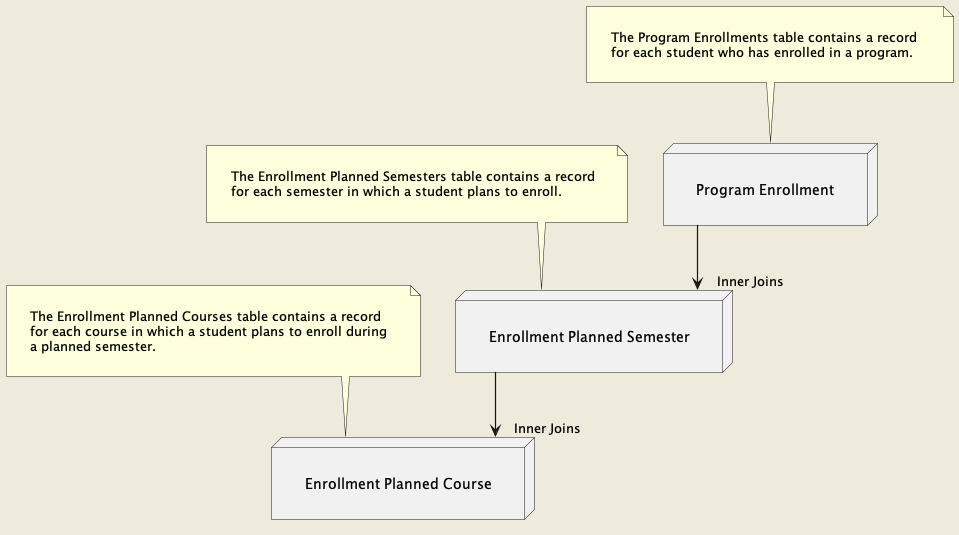
\includegraphics[max size={\textwidth}{\textheight}]{course-enrollment-demand}
    \caption{\textbf{Report Data Flow}}
\end{figure}

The \textit{Total Course Enrollments by Semester and Program} report will provide a count of the total planned course enrollments by semester and program, as shown in the figure below, which displays all planned course enrollments for the Fall 1 2023 semester.

\begin{figure}[ht]
    \centering
    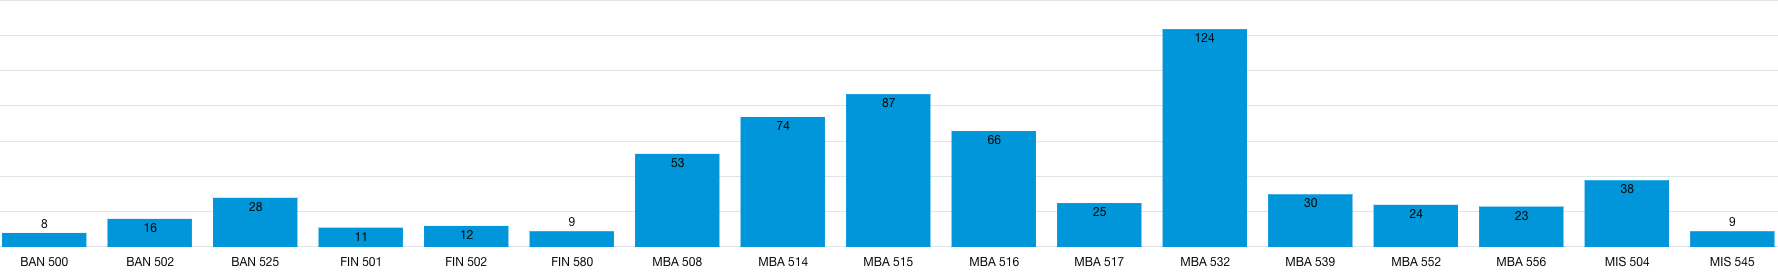
\includegraphics[max size={\textwidth}{\textheight}]{planned-courses}
    \label{fig:planned-courses}
    \caption{\textbf{Course Enrollment Demand Report}}
\end{figure}

Additionally, when the report is exported as a CSV file, the report data can be imported into a spreadsheet application, such as Microsoft Excel, to assign a course CRN to each planned course enrollment. By doing this, the operations team can easily create course sections for a given course based on the student's program. This information can be forwarded to the registrar's office during the mass course registration period to register students for courses. This is a significant improvement over the current process, which requires the operations team to manually register students for courses by sifting through numerous spreadsheets and manually entering student information into the registrar's system.

\begin{figure}[ht]
    \centering
    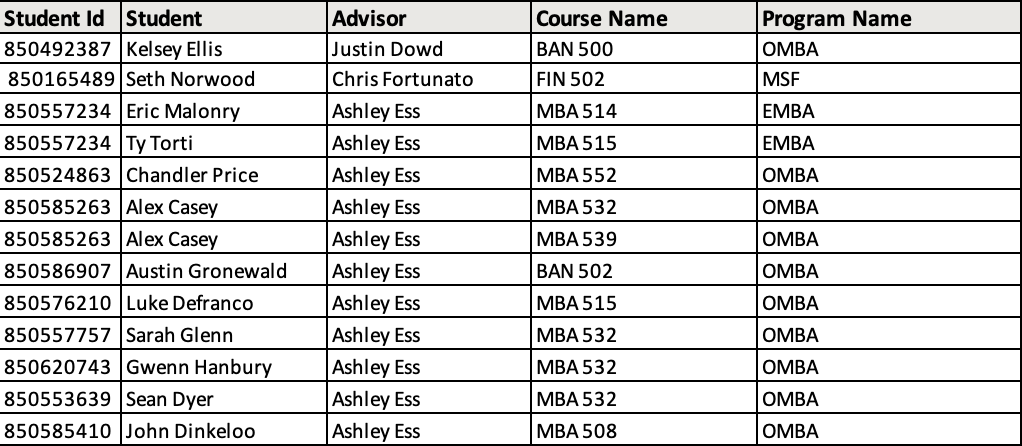
\includegraphics[max size={\textwidth}{\textheight}]{planned-course-csv-output}
    \label{fig:planned-course-csv-output}
    \caption{\textbf{Course Enrollment Demand Report CSV Output}}
\end{figure}

\section{Lessons Learned and Future Work}
\subsection{Lessons Learned}
Throughout the development of the OAP Operations and Advising System, a myriad of invaluable insights surfaced, shedding light on various aspects of software development and project management. One critical observation was the propensity for software development and deployment timeframes to surpass initial estimates, a phenomenon often attributed to unforeseen obstacles and the intrinsic complexities entwined with such processes.

In addition, the experience accentuated the importance of devoting sufficient time and resources to gathering detailed requirements and analyzing and establishing a sturdy data model foundation. Although the collection of requirements transpired continuously throughout the development lifecycle, the initial phase proved particularly crucial. This was primarily because the requirements were largely stable, with negligible scope creep or additional requests. A deep understanding of domain-specific requirements and system functionality was critical in ensuring the project's ultimate success.

Moreover, the project highlighted the value of incorporating user stories and use cases to enhance system comprehension. These methodological tools facilitated the visualization of user interactions with the system, identifying potential gaps or issues that may have been overlooked. Consequently, this created a more robust and user-centric solution that effectively addressed users' needs.

Lastly, the project emphasized the vital role of regular stakeholder meetings in fostering open discussion and gathering valuable feedback on the system. These collaborative sessions promoted transparent communication, ensured alignment with project objectives, and facilitated the implementation of necessary adjustments in response to evolving requirements or emerging challenges. The project team was better equipped to address concerns and deliver a successful solution by maintaining a strong feedback loop.

\subsection{Future Work}
For future work, prioritizing identifying a suitable individual or team to assume responsibility for continuous system maintenance and stewardship is crucial. This maintenance includes not only the integration of new features but also the swift resolution of any system bugs or glitches that may surface. Guaranteeing ongoing support and timely updates for the OAP Operations and Advising System is essential in sustaining its effectiveness and adaptability to the ever-changing demands of OAP programs and the dynamic landscape of the student experience.

By designating a committed team or individual to supervise the system's maintenance, the OAP Operations and Advising System can better adapt to emerging trends and technologies, ensuring its continued relevance and value to users. This long-term dedication to system support will also amplify user satisfaction. The system will be persistently improved and refined to address feedback, fulfill new expectations, and accommodate the evolving requirements of the OAP programs and their participants.

In conclusion, future developments must emphasize securing an appropriate party to oversee system maintenance and stewardship. This is a critical component in preserving the system's overall effectiveness and responsiveness to the shifting needs of its users and the broader OAP landscape.

\newpage
\begin{thebibliography}{l}
    \bibitem{b1} Gamma, E., Helm, R., Johnson, R. \& Vlissides, J. Design Patterns: Elements of Reusable Object-Oriented Software. (Addison-Wesley Professional,1994)
\end{thebibliography}

\newpage
\begin{appendices}
\section{Appendix A: Entity Relationship Diagram}
    \begin{figure*}[ht]
        \centering
        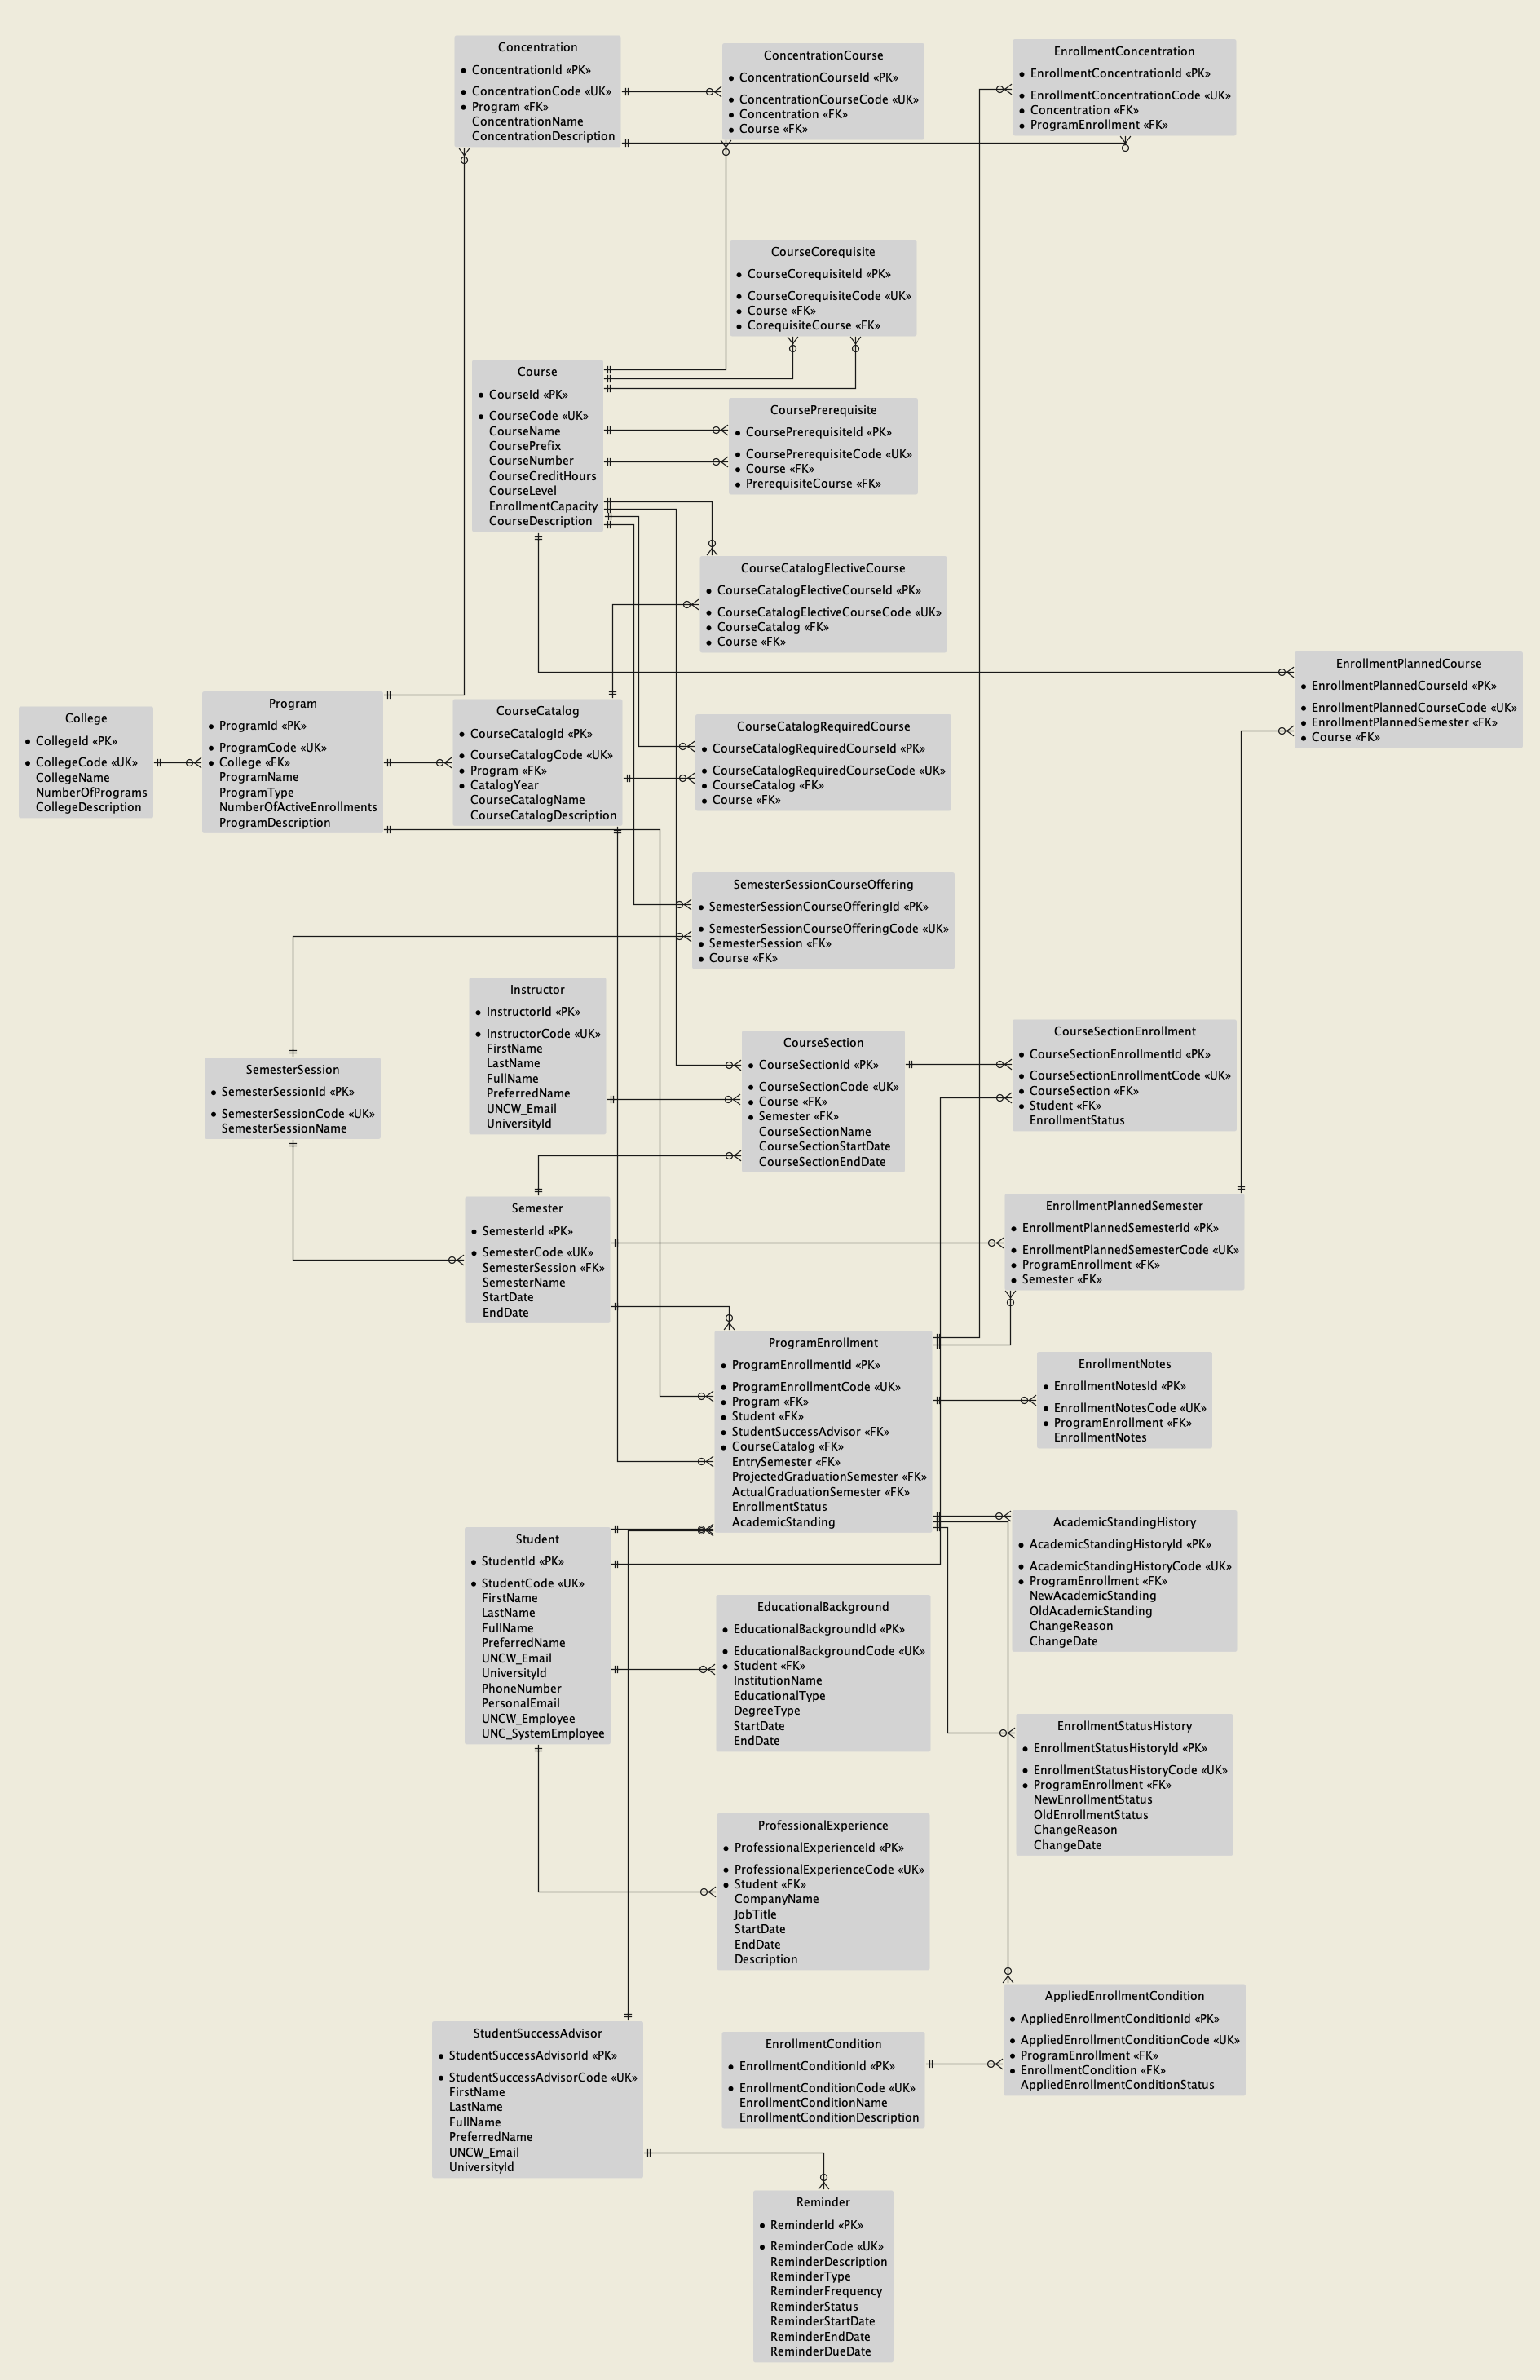
\includegraphics[trim={0 40cm 0 0},clip,width=\textwidth]{entity-relationship-diagram-with-attr}
        \caption{Entity Relationship Diagram}
        \label{fig:entity-relationship-diagram-with-attr1}
    \end{figure*}
    
    \begin{figure*}[ht]
        \ContinuedFloat
        \centering
            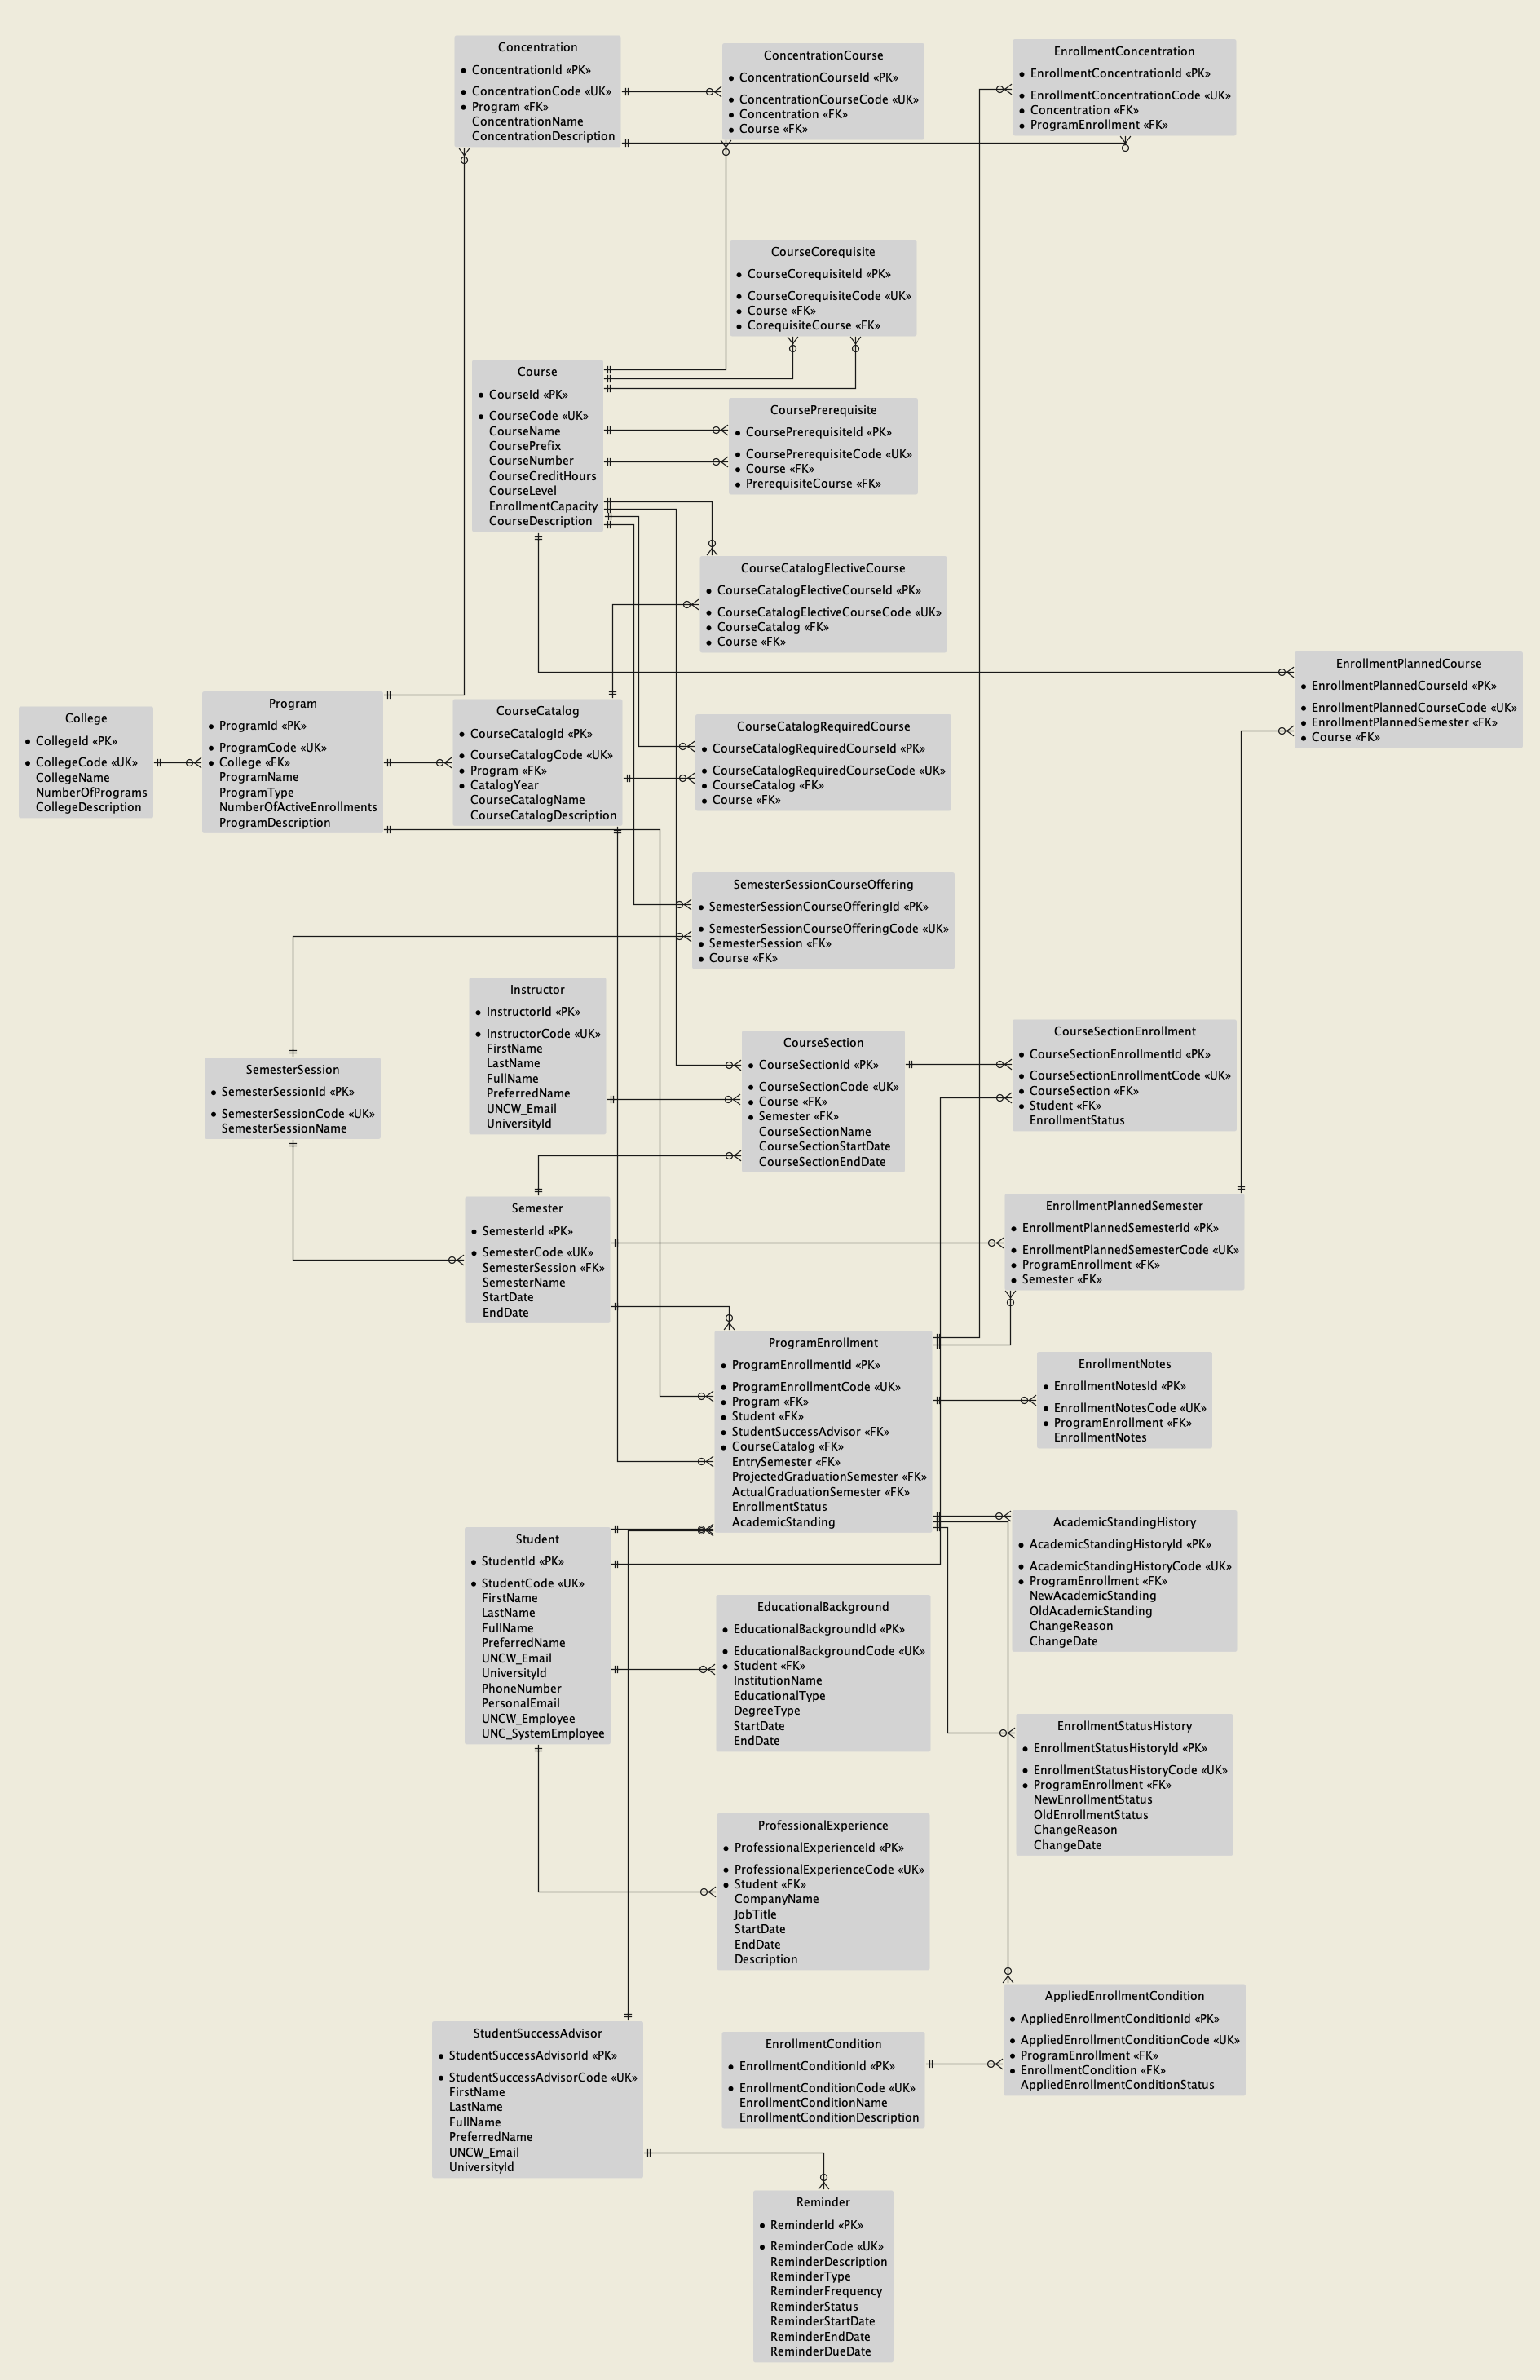
\includegraphics[trim={0 0 0 25cm},clip,width=\textwidth]{entity-relationship-diagram-with-attr}
        \caption{Continued from previous page}
        \label{fig:entity-relationship-diagram-with-attr2}
    \end{figure*}
    \restoregeometry

\section{Appendix B: Domain Class Diagram}
    \begin{figure}[ht]
        \centering
        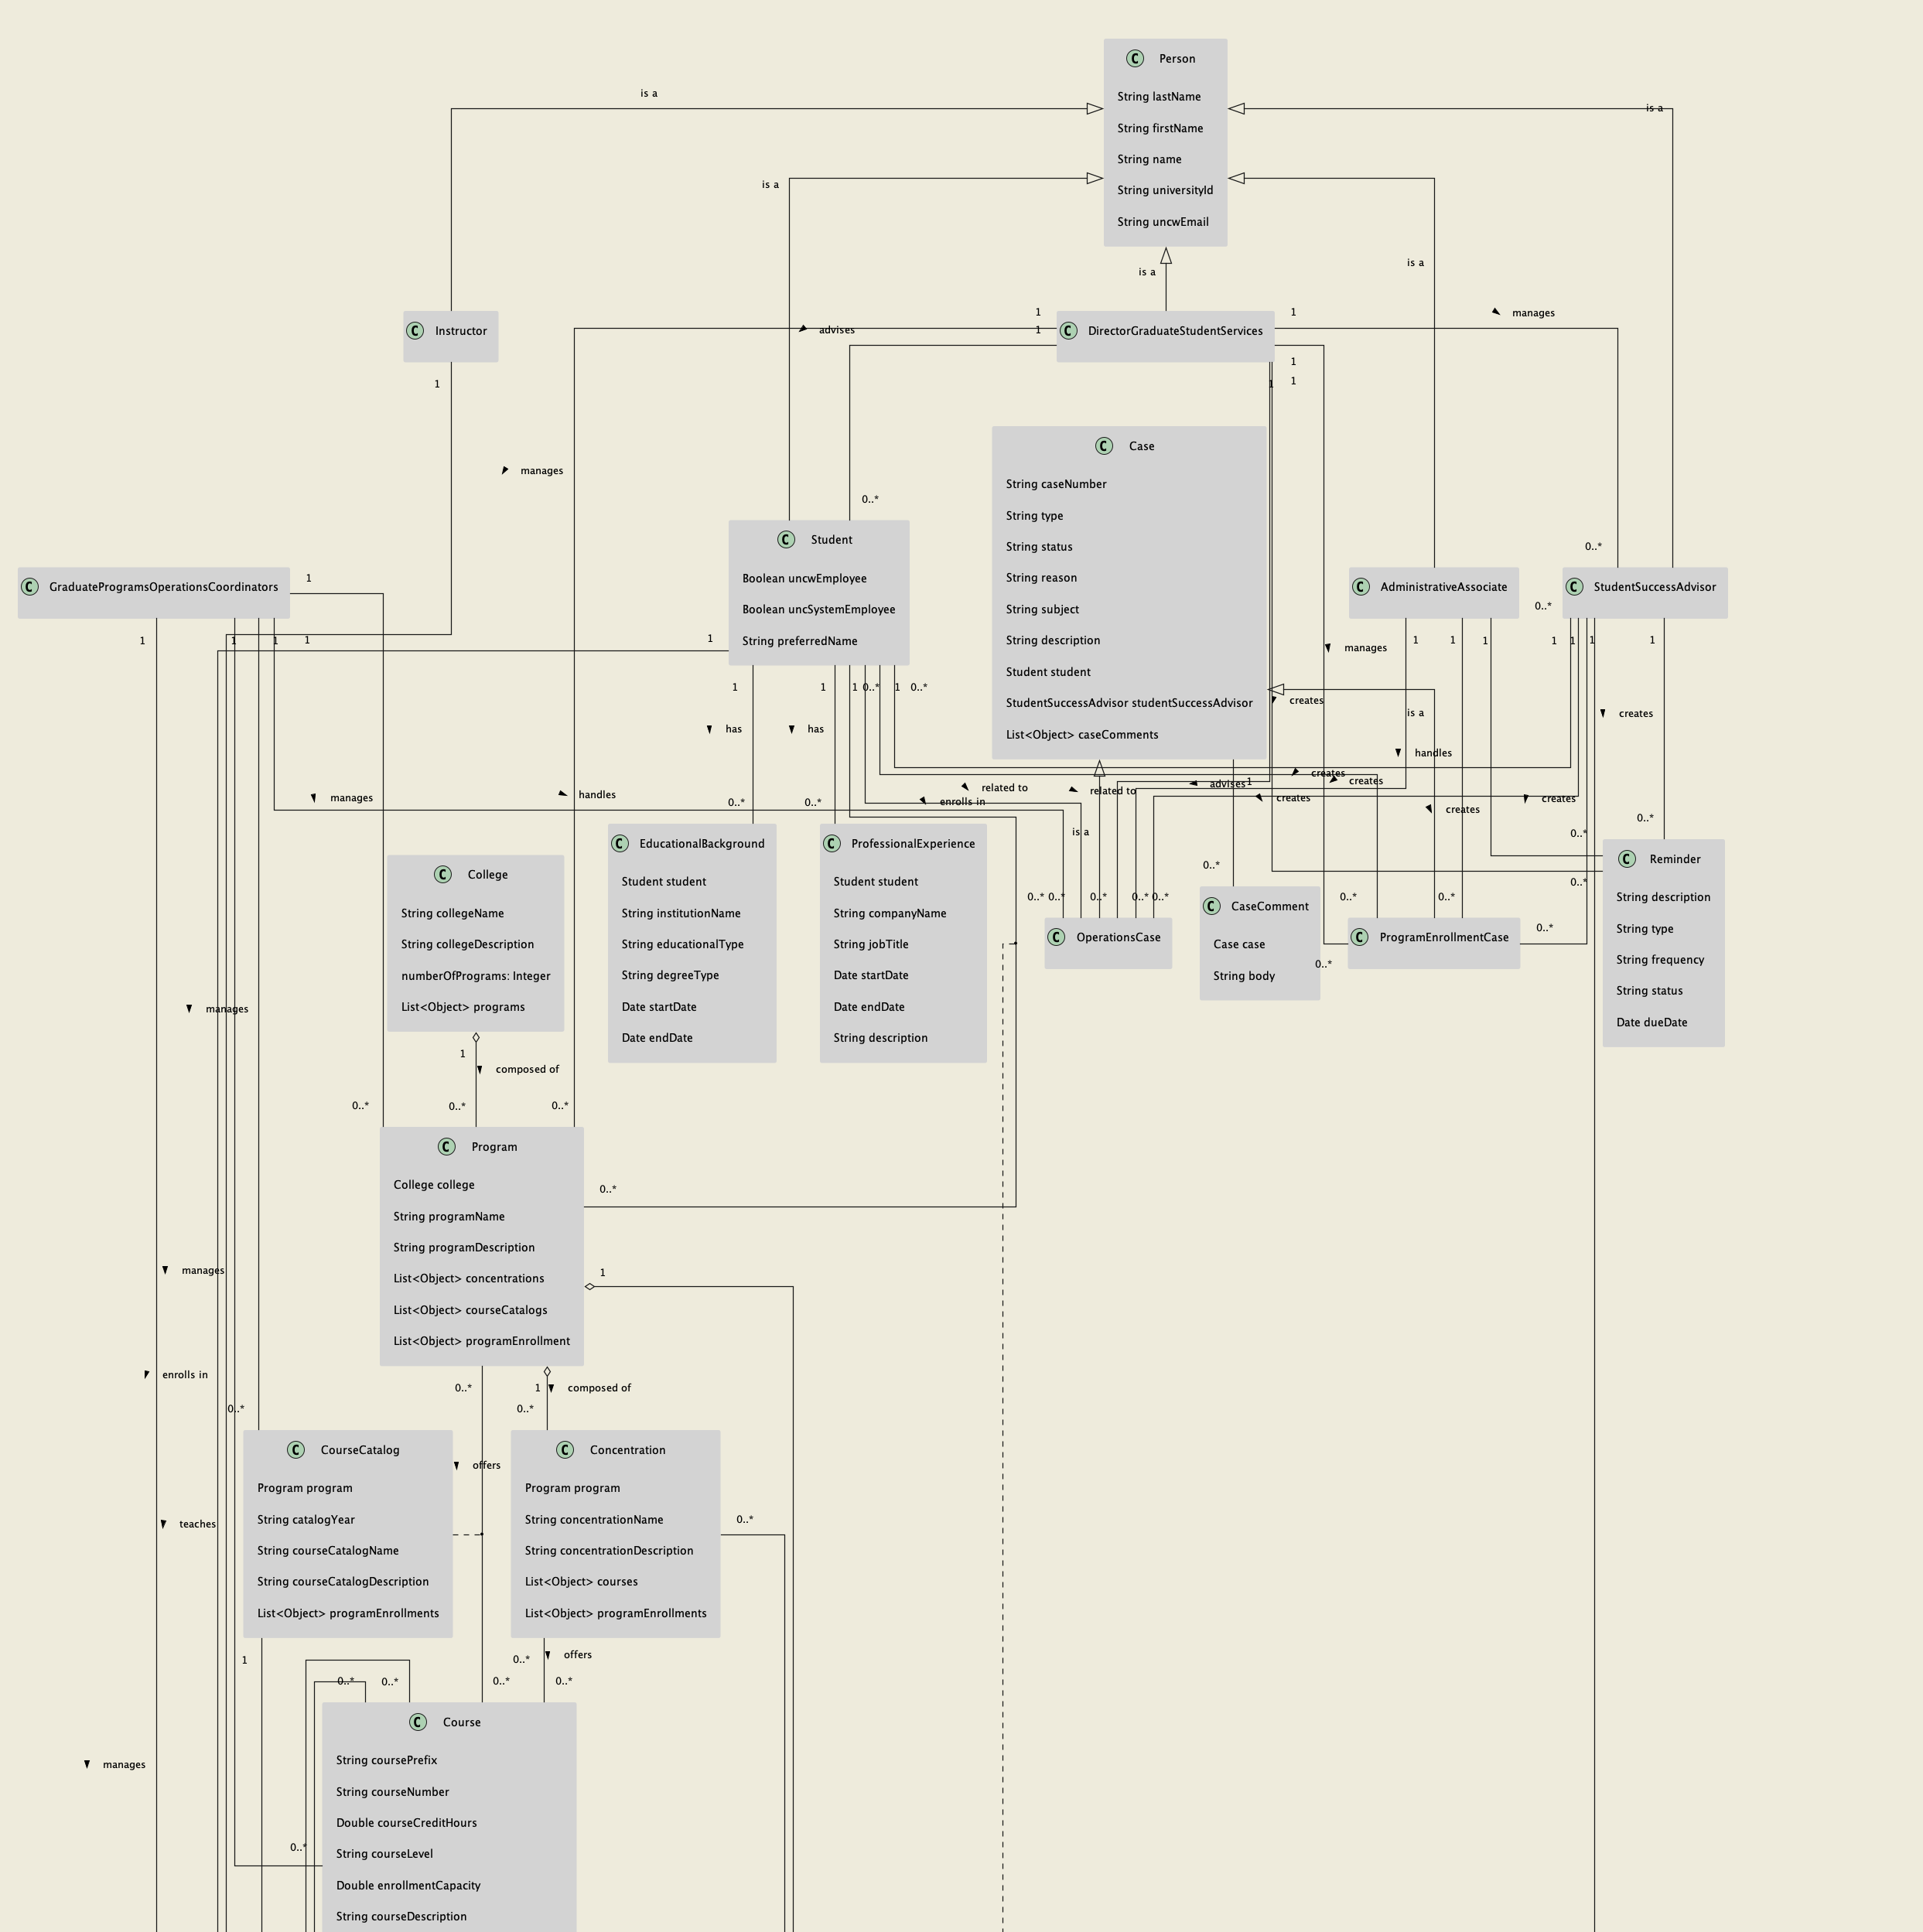
\includegraphics[max size = {\textwidth}{\textheight}]{domain-class-diagram-with-attr-1}
        \caption{Domain Class Diagram}
        \label{fig:domain-class-diagram-with-attr-1}
    \end{figure}
    \newpage
    \begin{figure}[ht]
        \centering
            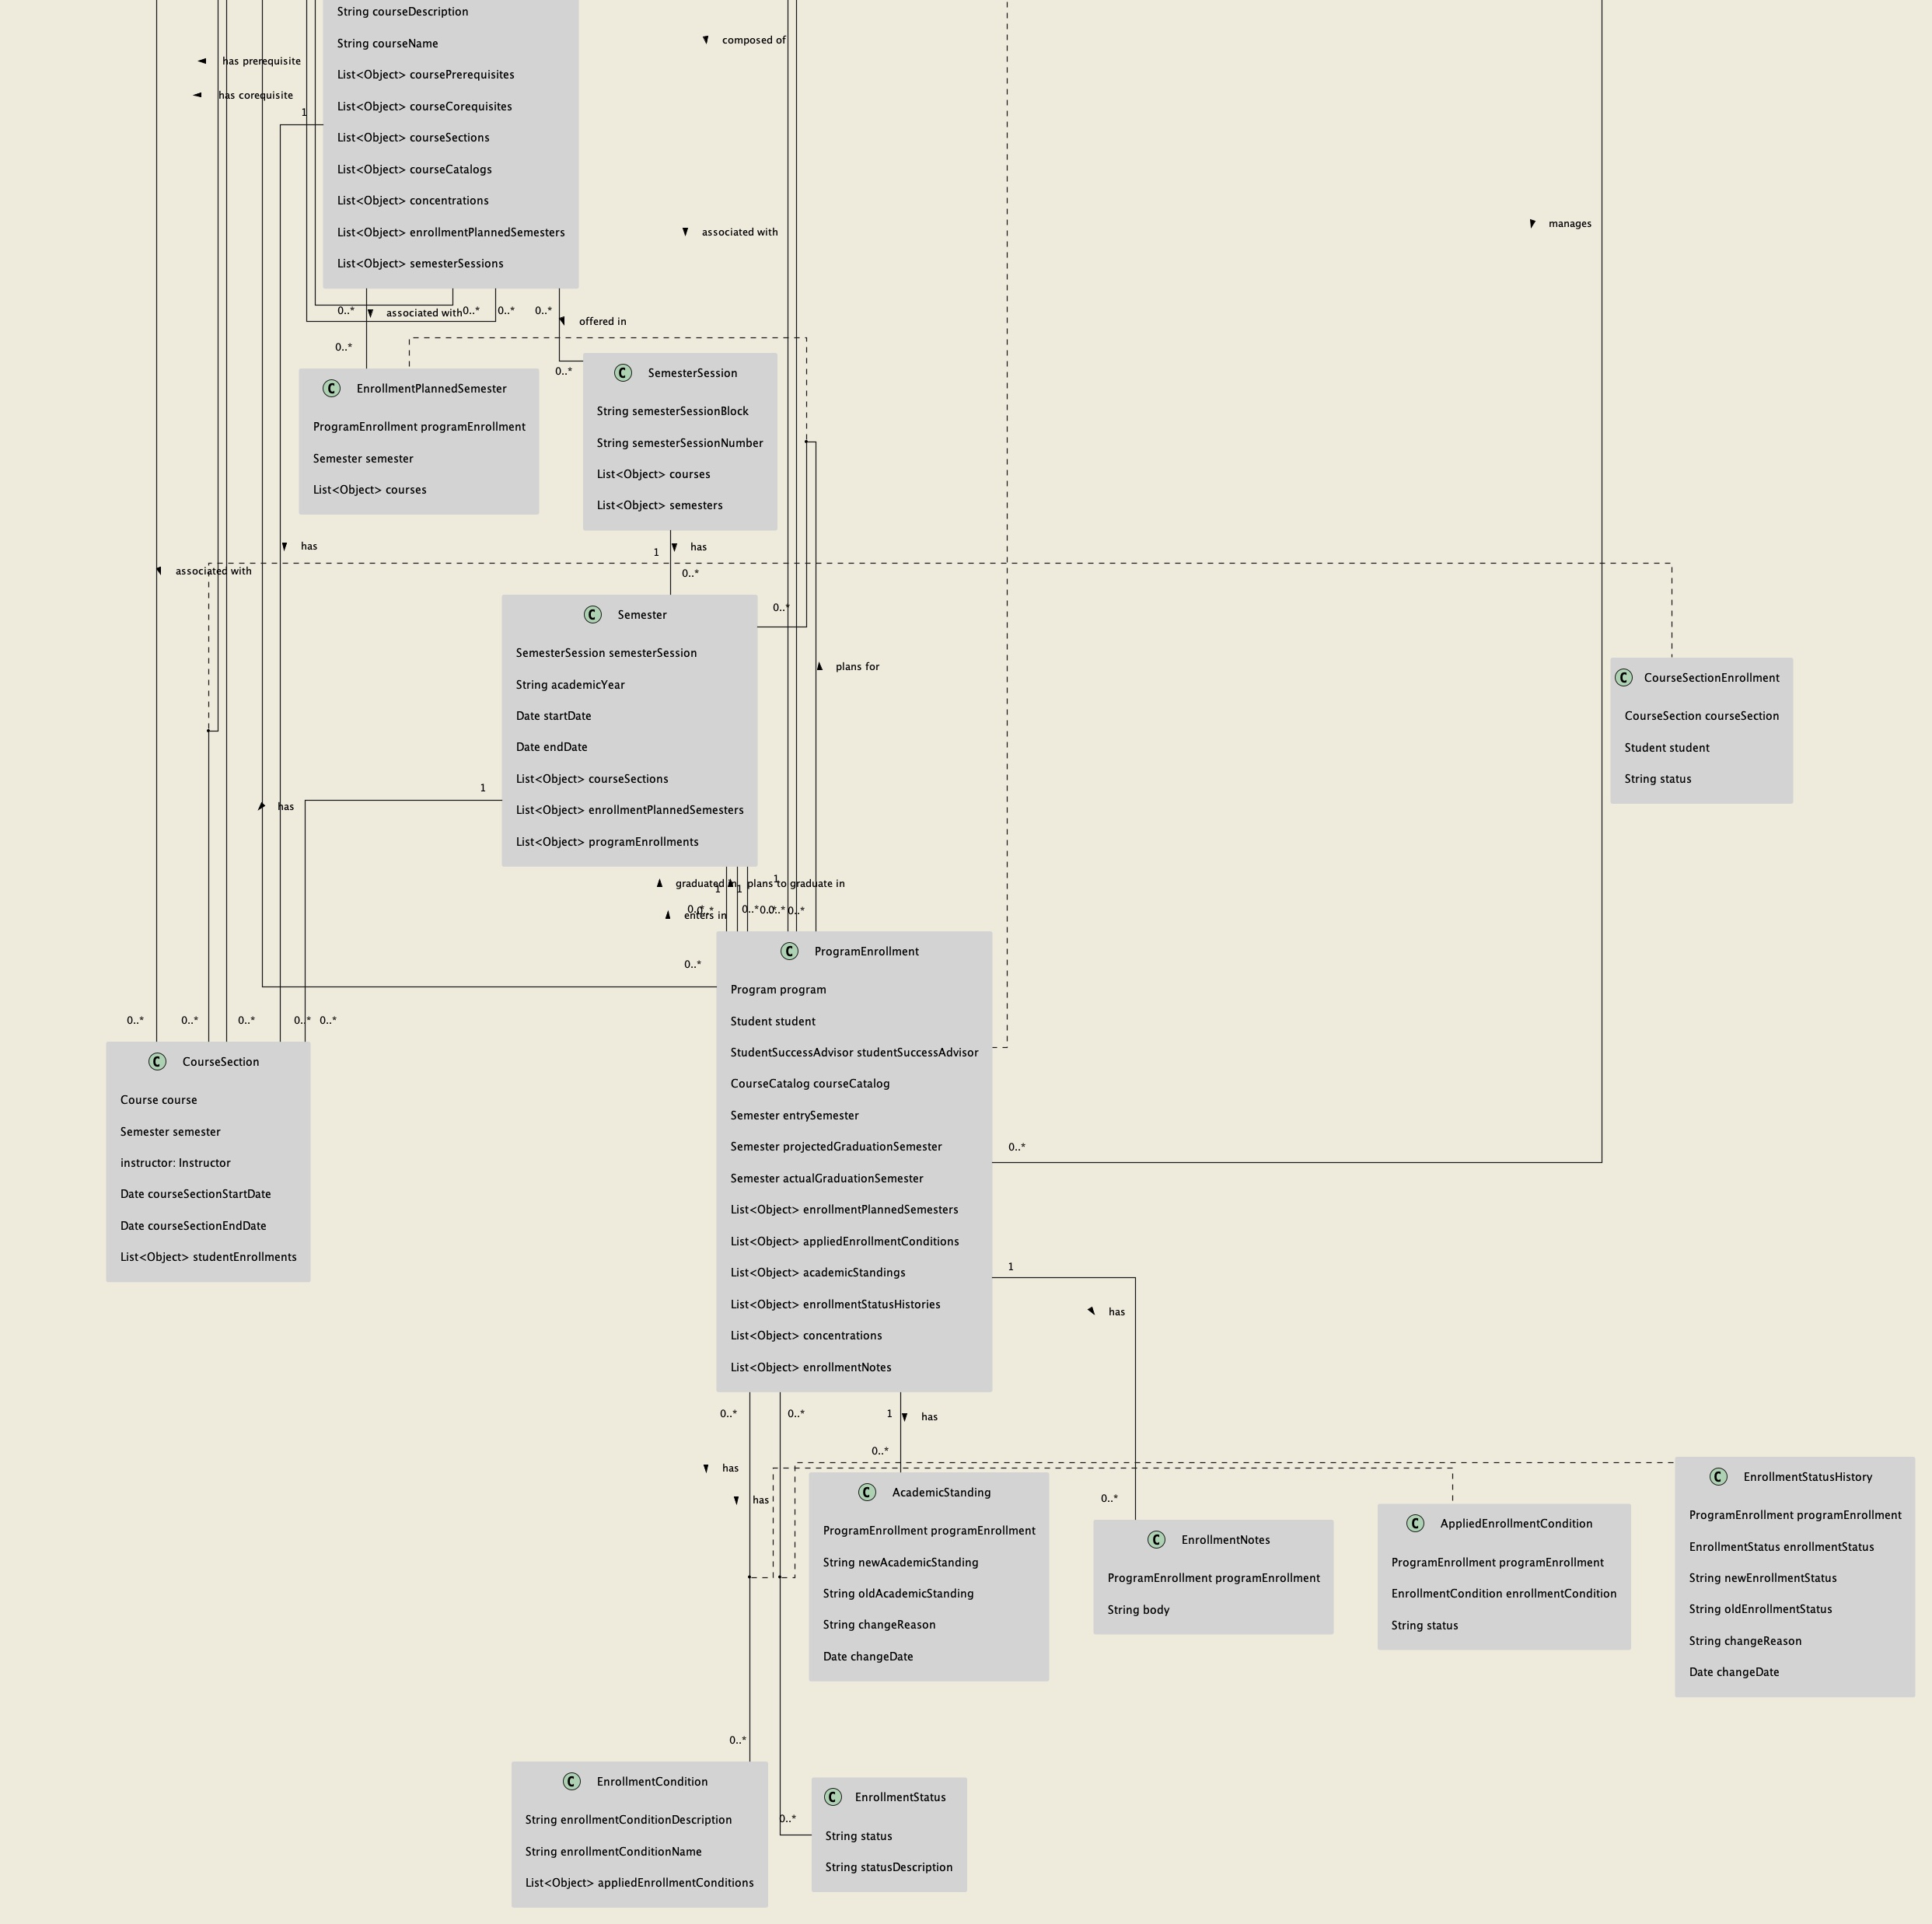
\includegraphics[max size = {\textwidth}{\textheight}]{domain-class-diagram-with-attr-2}
        \caption{Continued from previous page}
        \label{fig:domain-class-diagram-with-attr-2}
    \end{figure}
    
\section{Appendix C: Data Dictionary}
This data dictionary provides an overview of the entities and their attributes used in the OAP Operations and Advising System. It serves as a reference for understanding the system's structure and organization. Each entity has unique details that describe its role and function.

\begin{enumerate}[label=(\roman*)]
    \newpage
    \item \textbf{College}
    \item[] A college is an educational institution comprising various academic programs related to a common theme or discipline. For example, the Cameron School of Business is a college made up of several academic programs, such as the MBA, MS in Accounting, and MS in Finance. These programs are courses designed to provide students with learning objectives in a specific subject area and prepare them to earn a degree or certificate upon completion. Each college is associated with one or more programs, and the programs are typically organized and administered by the college.
    \item[] \textbf{Attributes}
    \begin{itemize}
        \item Id: The unique identifier for the college. (PK)
        \item CollegeCode: The unique code that identifies the college. (UK)
        \item CollegeName: The name of the college.
        \item CollegeDescription: A description of the college.
        \item NumberOfPrograms: The number of programs that belong to the college.
    \end{itemize}
    \begin{itemize}
        \item \textbf{Relationships}
        \item College $ \longrightarrow \langle has \hspace{0.125cm} many \rangle $  Program
    \end{itemize}

    \item \textbf{Program}
    \item[] A program is an organized set of courses designed to provide students with the knowledge and skills necessary to achieve specific learning objectives in a particular field. Upon completion of the program, students are eligible to receive a degree or certificate, typically earned by completing all required program coursework and meeting any additional requirements for graduation. Programs are affiliated with colleges, which are groups of academic programs that share a common theme or discipline, such as business or engineering. Each program has a course catalog, a comprehensive list of all the required or elective courses for a degree within that program. Some programs may also offer concentrations, which are focused sets of courses within the program that provide students with a more specialized learning experience in a particular area of interest. These concentrations may have additional requirements or elective courses that students must complete to satisfy the concentration.
    \item[] \textbf{Attributes}
    \begin{itemize}
        \item Id: The unique identifier for the program. (PK)
        \item ProgramCode: The unique code that identifies the program. (UK)
        \item College: The college to which the program belongs. (FK)
        \item ProgramName: The name of the program.
        \item ProgramDescription: A description of the program.
        \item ProgramType: The type of program (e.g., undergraduate, graduate).
        \item NumberOfActiveEnrollments: The number of active students enrolled in the program.
        \item NumberOfConcentrations: The number of concentrations that are associated with the 
    \end{itemize}
    \item[] \textbf{Relationships}
    \begin{itemize}
        \item Program $ \longrightarrow \langle has \hspace{0.125cm} one \rangle $ College
        \item Program $ \longrightarrow \langle has \hspace{0.125cm} many \rangle $ CourseCatalog
        \item Program $ \longrightarrow \langle has \hspace{0.125cm} many \rangle $ Concentration
        \item Program $ \longrightarrow \langle has \hspace{0.125cm} many \rangle $ ProgramEnrollment
    \end{itemize}

    \newpage
    \item \textbf{Concentration}
    \item[] A concentration is a specialized learning track within a particular academic program that allows students to focus their studies on a specific subject area. This can be particularly useful for students interested in gaining in-depth knowledge and expertise in a particular field within their chosen program of study. For example, a student enrolled in a Business Administration program may pursue a concentration in Marketing, requiring them to take courses focused on marketing principles and practices. These courses may cover market research, advertising, and branding topics and are designed to give students a deeper understanding of the field and help them develop specialized skills and knowledge. In addition to required courses, concentrations may include elective courses or other requirements that students must complete to fulfill the concentration requirements. Pursuing a concentration allows students to tailor their academic program to their specific interests and career goals. It can help them stand out in the job market by demonstrating a high level of expertise in a particular subject area.
    \item[] \textbf{Attributes}
    \begin{itemize}
        \item Id: The unique identifier for the concentration. (PK)
        \item ConcentrationCode: The unique code that identifies the concentration. (UK)
        \item Program: The program to which the concentration belongs. (FK)
        \item ConcentrationName: The name of the concentration.
        \item ConcentrationDescription: A description of the concentration.
    \end{itemize}
    \item[] \textbf{Relationships}
    \begin{itemize}
        \item Concentration $ \longrightarrow \langle has \hspace{0.125cm} one \rangle $ Program
        \item Concentration $ \longrightarrow \langle has \hspace{0.125cm} many \rangle $ ConcentrationCourse
        \item Concentration $ \longrightarrow \langle has \hspace{0.125cm} many \rangle $ EnrollmentConcentration
    \end{itemize}

    \item \textbf{Course}
    \item[] A course is a unit of study offered by a college or university as part of an academic program. It typically covers a specific subject area or topic and is designed to help students learn and master the material. To earn credit for a course, students must typically complete a set of assignments and assessments, such as exams, papers, or projects.

    Some courses may have prerequisites, which are other courses that a student must have completed before enrolling in the course in question. Prerequisites are often required to ensure that students have the necessary background knowledge and skills to succeed in the course. Similarly, some courses may have corequisites, which are other courses that can be taken concurrently with the course in question.
    
    To participate in a course, students must typically enroll in a specific offering of the course, known as a course section, during a particular semester. Course sections may be held in various formats, such as in-person or online, and may be scheduled at different times of the day or week to accommodate students' schedules.
    \item[] \textbf{Attributes}
    \begin{itemize}
        \item Id: The unique identifier for the course. (PK)
        \item CourseCode: The unique code that identifies the course. (UK)
        \item CourseName: The name of the course.
        \item CoursePrefix: The prefix is used to identify the course's subject area.
        \item CourseNumber: The number used to identify the specific course within the subject area.
        \item CourseCreditHours: The number of credit hours that the course is worth.
        \item EnrollmentCapacity: The maximum number of students can enroll in the course.
        \item CourseDescription: A description of the course.
    \end{itemize}
    \item[] \textbf{Relationships}
    \begin{itemize}
        \item Course $ \longrightarrow \langle has \hspace{0.125cm} many \rangle $ CourseCorequisite
        \item Course $ \longrightarrow \langle has \hspace{0.125cm} many \rangle $ CoursePrerequisite
        \item Course $ \longrightarrow \langle has \hspace{0.125cm} many \rangle $ CourseSection
        \item Course $ \longrightarrow \langle has \hspace{0.125cm} many \rangle $ ConcentrationCourse
        \item Course $ \longrightarrow \langle has \hspace{0.125cm} many \rangle $ EnrollmentPlannedCourse
        \item Course $ \longrightarrow \langle has \hspace{0.125cm} many \rangle $ SemesterSessionCourseOffering
        \item Course $ \longrightarrow \langle has \hspace{0.125cm} many \rangle $ CourseCatalogRequiredCourse
        \item Course $ \longrightarrow \langle has \hspace{0.125cm} many \rangle $ CourseCatalogElectiveCourse
    \end{itemize}

    \item \textbf{Course Catalog}
    \item[] A course catalog is a detailed list of courses offered by a particular academic program that students can take to fulfill their degree requirements. It includes both required courses, which are mandatory for all students in the program, and elective courses, which allow students to choose from a selection of courses to customize their learning experience. The course catalog provides information about each course, including its description, prerequisites (courses that must be completed before taking a particular course), and corequisites (courses that must be taken concurrently with a specific course). 

    The course catalog reflects its program's curriculum and requirements. The course catalog is a tool for students and advisers to plan a student's course schedule, as it outlines the courses required or optional for the student's specific program enrollment.
    \item[] \textbf{Attributes}
    \begin{itemize}
        \item Id: The unique identifier for the course catalog. (PK)
        \item CourseCatalogCode: The unique code that identifies the course catalog. (UK)
        \item Program: The program to which the course catalog belongs. (FK)
        \item CatalogYear: The academic year for which the course catalog applies.
        \item CourseCatalogName: The name of the course catalog.
        \item CourseCatalogDescription: A description of the course catalog.
    \end{itemize}
    \item[] \textbf{Relationships}
    \begin{itemize}
        \item CourseCatalog $ \longrightarrow \langle has \hspace{0.125cm} one \rangle $ Program
        \item CourseCatalog $ \longrightarrow \langle has \hspace{0.125cm} many \rangle $ CourseCatalogRequiredCourse
        \item CourseCatalog $ \longrightarrow \langle has \hspace{0.125cm} many \rangle $ CourseCatalogElectiveCourse
        \item CourseCatalog $ \longrightarrow \langle has \hspace{0.125cm} many \rangle $ ProgramEnrollment
    \end{itemize}

    \item \textbf{Course Catalog Required Course}
    \item[] A course catalog required course is a course that is mandatory for students enrolled in a specific degree program to complete to fulfill their requirements for earning the degree. These courses are required for a student to fulfill program requirements. A course catalog required course is a line item in the course catalog.
    \item[] \textbf{Attributes}
    \begin{itemize}
        \item Id: The unique identifier for the course catalog required course. (PK)
        \item CourseCatalogRequiredCourseCode: The unique code that identifies the course catalog required course. (UK)
        \item CourseCatalog: The course catalog to which the required course belongs. (FK)
        \item Course: The course that is required for the degree. (FK)
    \end{itemize}
    \item[] \textbf{Relationships}
    \begin{itemize}
        \item CourseCatalogRequiredCourse $ \longrightarrow \langle has \hspace{0.125cm} one \rangle $ CourseCatalog
        \item CourseCatalogRequiredCourse $ \longrightarrow \langle has \hspace{0.125cm} one \rangle $ Course
    \end{itemize}

    \item \textbf{Course Catalog Elective Course}
    \item[] A course catalog elective course is a course listed in a course catalog as an optional choice for students to take as part of their degree program. These courses are usually optional for a student to graduate but can be taken to fulfill program requirements or to allow students to explore different subjects of interest. A course catalog elective course is a line item in the course catalog.
    \item[] \textbf{Attributes}
    \begin{itemize}
        \item Id: The unique identifier for the course catalog elective course. (PK)
        \item CourseCatalogElectiveCourseCode: The unique code that identifies the course catalog elective course. (UK)
        \item CourseCatalog: The course catalog includes the elective course as an option. (FK)
        \item Course: The course is listed as an elective in the course catalog. (FK)
    \end{itemize}
    \item[] \textbf{Relationships}
    \begin{itemize}
        \item CourseCatalogRequiredCourse $ \longrightarrow \langle has \hspace{0.125cm} one \rangle $ CourseCatalog
        \item CourseCatalogRequiredCourse $ \longrightarrow \langle has \hspace{0.125cm} one \rangle $ Course
    \end{itemize}

    \item \textbf{Concentration Course}
    \item[] A concentration course is a course that is related to a specific concentration within a program. Students who have chosen to pursue a concentration as part of their program enrollment must complete a set of concentration courses to fulfill the concentration requirements and gain specialized knowledge and skills in a particular subject area. In order to complete the concentration, students must take two courses specified by their concentration.
    \item[] \textbf{Attributes}
    \begin{itemize}
        \item Id: The unique identifier for the concentration course. (PK)
        \item ConcentrationCourseCode: The unique code that identifies the concentration course. (UK)
        \item Concentration: The concentration to which the course belongs. (FK)
        \item Course: The course that is part of the concentration. (FK)
    \end{itemize}
    \item[] \textbf{Relationships}
    \begin{itemize}
        \item * ConcentrationCourse $ \longrightarrow \langle has \hspace{0.125cm} one \rangle $ Concentration
        \item * ConcentrationCourse $ \longrightarrow \langle has \hspace{0.125cm} one \rangle $ Course
    \end{itemize}

    \item \textbf{Course Corequisite}
    \item[] A course corequisite is a course that a student can take concurrently with another. This is often used to ensure students have the necessary background knowledge or skills to succeed in a course. For instance, a student may be required to take a corequisite course to enroll in a course that requires them to use a particular software program. This arrangement allows students to gain the necessary skills and knowledge while taking the main course.
    \item[] \textbf{Attributes}
    \begin{itemize}
        \item Id: The unique identifier for the course corequisite. (PK)
        \item CourseCorequisiteCode: The unique code that identifies the course corequisite. (UK)
        \item Course: The course that has the corequisite. (FK)
        \item CorequisiteCourse: The course that is the corequisite. (FK)
    \end{itemize}
    \item[] \textbf{Relationships}
    \begin{itemize}
        \item CourseCorequisite $ \longrightarrow \langle has \hspace{0.125cm} one \rangle $ Course
        \item CourseCorequisite $ \longrightarrow \langle has \hspace{0.125cm} one \rangle $ CorequisiteCourse
    \end{itemize}

    \item \textbf{Course Prerequisite}
    \item[] A course prerequisite is a requirement a student must fulfill before enrolling in a particular course. This means that the student must complete a specified course before they are eligible to enroll in the other course. This requirement is often put in place to ensure that students have the necessary background knowledge or skills to succeed in the course they wish to enroll in. For example, a student may need to take a prerequisite course to enroll in a course requiring them to use a specific software program that requires a certain level of proficiency. This arrangement allows students to gain the necessary skills and knowledge before they take the main course.
    \item[] \textbf{Attributes}
    \begin{itemize}
        \item Id: The unique identifier for the course prerequisite. (PK)
        \item CoursePrerequisiteCode: The unique code that identifies the course prerequisite. (UK)
        \item Course: The course that has the prerequisite. (FK)
        \item PrerequisiteCourse: The course that is the prerequisite. (FK)
    \end{itemize}
    \item[] \textbf{Relationships}
    \begin{itemize}
        \item CoursePrerequisite $ \longrightarrow \langle has \hspace{0.125cm} one \rangle $ Course
        \item CoursePrerequisite $ \longrightarrow \langle has \hspace{0.125cm} one \rangle $ PrerequisiteCourse
    \end{itemize}

    \item \textbf{Program Enrollment}
    \item[] A program enrollment records a student's enrollment in a program. It includes details about the student's academic standing, enrollment status, and any conditions that must be met for the student to remain enrolled in the program. It also outlines the semesters the student has planned for and the courses that will be taken during a planned semester. 

    Additionally, a program enrollment may include information about the student's assigned student success advisor, who is responsible for providing academic guidance and support to the student throughout their enrollment in the program. It may also include details about the student's planned semesters for completing the program, including which courses they will take each semester and when they expect to graduate. Students may have multiple program enrollments, as they may enroll in and drop out of different programs or enroll in new ones after completing their previous program.
    \item[] \textbf{Attributes}
    \begin{itemize}
        \item Id: The unique identifier for the program enrollment. (PK)
        \item ProgramEnrollmentCode: The unique code that identifies the program enrollment. (UK)
        \item Program: The program that the student is enrolled in. (FK)
        \item Student: The student who is enrolled in the program. (FK)
        \item StudentSuccessAdvisor: The adviser who is assigned to the student. (FK)
        \item CourseCatalog: The course catalog applies to the student's program enrollment. (FK)
        \item EntrySemester: The semester during which the student began their program. (FK)
        \item ProjectedGraduationSemester: The semester during which the student is expected to graduate. (FK)
        \item ActualGraduationSemester: The semester during which the student graduated. (FK)
        \item EnrollmentStatus: The current status of the student's enrollment in the program (e.g., active, withdrawn, graduated).
        \item AcademicStanding: The student's current academic standing (e.g., good standing, probation, suspension).
    \end{itemize}
    \item[] \textbf{Relationships}
    \begin{itemize}
        \item ProgramEnrollment $ \longrightarrow \langle has \hspace{0.125cm} one \rangle $ Program
        \item ProgramEnrollment $ \longrightarrow \langle has \hspace{0.125cm} one \rangle $ Student
        \item ProgramEnrollment $ \longrightarrow \langle has \hspace{0.125cm} one \rangle $ StudentSuccessAdvisor
        \item ProgramEnrollment $ \longrightarrow \langle has \hspace{0.125cm} one \rangle $ CourseCatalog
        \item ProgramEnrollment $ \longrightarrow \langle has \hspace{0.125cm} one \rangle $ EntrySemester (Semester)
        \item ProgramEnrollment $ \longrightarrow \langle has \hspace{0.125cm} one \rangle $ ProjectedGraduationSemester (Semester)
        \item ProgramEnrollment $ \longrightarrow \langle has \hspace{0.125cm} one \rangle $ ActualGraduationSemester (Semester)
        \item ProgramEnrollment $ \longrightarrow \langle has \hspace{0.125cm} many \rangle $ EnrollmentPlannedSemester
        \item ProgramEnrollment $ \longrightarrow \langle has \hspace{0.125cm} many \rangle $ AppliedEnrollmentCondition
        \item ProgramEnrollment $ \longrightarrow \langle has \hspace{0.125cm} many \rangle $ AcademicStandingHistory
        \item ProgramEnrollment $ \longrightarrow \langle has \hspace{0.125cm} many \rangle $ EnrollmentConcentration
        \item ProgramEnrollment $ \longrightarrow \langle has \hspace{0.125cm} many \rangle $ EnrollmentStatusHistory
        \item ProgramEnrollment $ \longrightarrow \langle has \hspace{0.125cm} many \rangle $ EnrollmentNotes
    \end{itemize}

    \item \textbf{Enrollment Notes}
    \item[] An enrollment note is a note that is associated with a student's enrollment in a program. This note may include information about the student's academic standing, enrollment status, or any conditions that must be met for the student to remain enrolled in the program. It may also include details about the student's planned semesters for completing the program, including which courses they will take each semester and when they expect to graduate. Students may have multiple enrollment notes, as they may enroll in and drop out of different programs or enroll in new ones after completing their previous program.
    \item[] \textbf{Attributes}
    \begin{itemize}
        \item Id: The unique identifier for the enrollment note. (PK)
        \item EnrollmentNoteCode: The unique code that identifies the enrollment note. (UK)
        \item ProgramEnrollment: The program enrollment to which the enrollment note applies. (FK)
        \item Body: The body of the enrollment note.
    \end{itemize}
    \item[] \textbf{Relationships}
    \begin{itemize}
        \item EnrollmentNote $ \longrightarrow \langle has \hspace{0.125cm} one \rangle $ ProgramEnrollment
    \end{itemize}

    \item \textbf{Enrollment Planned Semester}
    \item[] A planned enrollment semester is a semester in which a student has planned to take courses as part of their academic program. This may include past, current, and future semesters in which the student has planned to take courses. These planned enrollment semesters are typically included in a student's academic plan or schedule, which outlines the courses they will take to graduate on time.
    \item[] \textbf{Attributes}
    \begin{itemize}
        \item Id: The unique identifier for the enrollment planned semester. (PK)
        \item EnrollmentPlannedSemesterCode: The unique code that identifies the enrollment planned semester. (UK)
        \item ProgramEnrollment: The program enrollment to which the planned semester applies. (FK)
        \item Semester: The semester during which the student plans to take the courses. (FK)
    \end{itemize}
    \item[] \textbf{Relationships}
    \begin{itemize}
        \item EnrollmentPlannedSemester $ \longrightarrow \langle has \hspace{0.125cm} one \rangle $ ProgramEnrollment
        \item EnrollmentPlannedSemester $ \longrightarrow \langle has \hspace{0.125cm} one \rangle $ Semester
        \item EnrollmentPlannedSemester $ \longrightarrow \langle has \hspace{0.125cm} many \rangle $ EnrollmentPlannedCourse
    \end{itemize}

    \item \textbf{Enrollment Planned Course}
    \item[] An enrollment planned course is a course a student has planned to take during a specific semester of their academic program. This may include required courses for the program and elective courses that the student has chosen to take to fulfill their degree requirements. These planned courses are typically included in a student's academic plan or schedule, which outlines the courses they will take each semester to graduate on time.
    \item[] \textbf{Attributes}
    \begin{itemize}
        \item Id: The unique identifier for the enrollment planned course. (PK)
        \item EnrollmentPlannedCourseCode: The unique code that identifies the enrollment planned course. (UK)
        \item EnrollmentPlannedSemester: The semester in which the course is planned to be taken. (FK)
        \item Course: The course that is planned to be taken. (FK)
    \end{itemize}
    \item[] \textbf{Relationships}
    \begin{itemize}
        \item EnrollmentPlannedCourse $ \longrightarrow \langle has \hspace{0.125cm} one \rangle $ EnrollmentPlannedSemester
        \item EnrollmentPlannedCourse $ \longrightarrow \langle has \hspace{0.125cm} one \rangle $ Course
    \end{itemize}

    \item \textbf{Enrollment Condition}
    \item[] Enrollment conditions are requirements that must be met for a student to be eligible to continue their enrollment in a particular program. These conditions can impact a student's ability to enroll in courses and progress toward their degree. Enrollment conditions may be based on a student's previous academic performance, completion of prerequisite courses, or fulfillment of other requirements. These requirements are typically set by the college or program and must be met by students to be accepted.
    \item[] \textbf{Attributes}
    \begin{itemize}
        \item Id: The unique identifier for the enrollment condition. (PK)
        \item EnrollmentConditionCode: The unique code that identifies the enrollment condition. (UK)
        \item EnrollmentConditionDescription: A description of the enrollment condition.
    \end{itemize}
    \item[] \textbf{Relationships}
    \begin{itemize}
        \item EnrollmentCondition $ \longrightarrow \langle has \hspace{0.125cm} many \rangle $ AppliedEnrollmentCondition
    \end{itemize}

    \item \textbf{Applied Enrollment Condition}
    \item[] An applied enrollment condition is a requirement or constraint that is applied to a student's program enrollment. A program enrollment may have multiple applied enrollment conditions, which are used to ensure that students meet the requirements for enrollment in the program and are able to progress toward graduation. These conditions can impact a student's ability to enroll in courses and move forward in their degree program.
    \item[] \textbf{Attributes}
    \begin{itemize}
        \item Id: The unique identifier for the applied enrollment condition. (PK)
        \item AppliedEnrollmentConditionCode: The unique code that identifies the applied enrollment condition. (UK)
        \item ProgramEnrollment: The program enrollment to which the enrollment condition has been applied. (FK)
        \item EnrollmentCondition: The enrollment condition that has been applied. (FK)
        \item Status: The current status of the applied enrollment condition (e.g., pending, satisfied, not satisfied, waived).
    \end{itemize}
    \item[] \textbf{Relationships}
    \begin{itemize}
        \item AppliedEnrollmentCondition $ \longrightarrow \langle has \hspace{0.125cm} one \rangle $ ProgramEnrollment
        \item AppliedEnrollmentCondition $ \longrightarrow \langle has \hspace{0.125cm} one \rangle $ EnrollmentCondition
    \end{itemize}

    \item \textbf{Educational Background}
    \item[] A student's educational background is the collection of institutions they have attended and qualifications they have obtained, such as high school diplomas, bachelor's degrees, master's degrees, etc.
    \item[] \textbf{Attributes}
    \begin{itemize}
        \item Id: The unique identifier for the educational background. (PK)
        \item EducationalBackgroundCode: The unique code that identifies the educational background. (UK)
        \item Student: The student whose educational background is being recorded. (FK)
        \item InstitutionName: The name of the institution where the student completed their highest level of education.
        \item EducationalType: The type of educational background (e.g., High School, College, Graduate, Doctoral).
        \item DegreeType: The type of degree the student received (e.g., Associate of Arts, Associate of Science, Bachelor of Arts, Bachelor of Science, Master of Arts, Master of Science, Doctor of Philosophy).
        \item StartDate: The date the student began their highest level of education.
        \item EndDate: The date the student completed their highest level of education.
    \end{itemize}
    \item[] \textbf{Relationships}
    \begin{itemize}
        \item EducationalBackground $ \longrightarrow \langle has \hspace{0.125cm} one \rangle $ Student
    \end{itemize}

    \item \textbf{Academic Standing History}
    \item[] The academic standing history is a record of the changes in a student's academic standing during their program enrollment over time. Whenever the student's academic standing changes, a new record is created to capture the change, which includes information about the reason for the change and the date it occurred. The academic standing history is related to the student's program enrollment and includes the academic standing that was assigned to the student at the time of the change. This history is often used to track a student's progress and ensure that they meet their program's requirements.
    \item[] \textbf{Attributes}
    \begin{itemize}
        \item Id: The unique identifier for the academic standing history record. (PK)
        \item AcademicStandingHistoryCode: The unique code that identifies the academic standing history record. (UK)
        \item ProgramEnrollment: The program enrollment for which the academic standing history applies. (FK)
        \item NewAcademicStanding: The academic standing that was assigned to the student at the time of the change.
        \item OldAcademicStanding: The academic standing that the student had before the change.
        \item ChangeReason: The reason for the academic standing change.
        \item ChangeDate: The date on which the academic standing change occurred.
    \end{itemize}
    \item[] \textbf{Relationships}
    \begin{itemize}
        \item AcademicStandingHistory $ \longrightarrow \langle has \hspace{0.125cm} one \rangle $ ProgramEnrollment
    \end{itemize}

    \item \textbf{Enrollment Status History}
    \item[] A student's enrollment status history is a record of the changes in their program enrollment over time. This can include enrollment statuses such as "Enrolled," "Dropped," and "Graduated." The enrollment status history consists of the reasons for these changes and captures the date. This history is often used to track a student's progress and ensure that they meet their program's requirements.
    \item[] \textbf{Attributes}
    \begin{itemize}
        \item Id: The unique identifier for the enrollment status history record. (PK)
        \item EnrollmentStatusHistoryCode: The unique code that identifies the enrollment status history record. (UK)
        \item ProgramEnrollment: The program enrollment for which the enrollment status history applies. (FK)
        \item NewEnrollmentStatus: The enrollment status that was assigned to the student at the time of the change.
        \item OldEnrollmentStatus: The enrollment status that the student had before the change.
        \item ChangeReason: The reason for the enrollment status change.
        \item ChangeDate: The date on which the enrollment status change occurred.        
    \end{itemize}
    \item[] \textbf{Relationships}
    \begin{itemize}
        \item EnrollmentStatusHistory $ \longrightarrow \langle has \hspace{0.125cm} one \rangle $ ProgramEnrollment
    \end{itemize}

    \item \textbf{Enrollment Concentration}
    \item[] An enrollment concentration is associated with a student's program enrollment. In order to fulfill the requirements of their enrollment concentration, a student must take two courses in that concentration. A student may have multiple enrollment concentrations within their program enrollment.
    \item[] \textbf{Attributes}
    \begin{itemize}
        \item Id: The unique identifier for the enrollment concentration. (PK)
        \item EnrollmentConcentrationCode: The unique code that identifies the enrollment concentration. (UK)
        \item ProgramEnrollment: The program enrollment for which the enrollment concentration applies. (FK)
        \item Concentration: The concentration that the student is enrolled in. (FK)
    \end{itemize}
    \item[] \textbf{Relationships}
    \begin{itemize}
        \item EnrollmentConcentration $ \longrightarrow \langle has \hspace{0.125cm} one \rangle $ ProgramEnrollment
        \item EnrollmentConcentration $ \longrightarrow \langle has \hspace{0.125cm} one \rangle $ Concentration
    \end{itemize}

    \item \textbf{Professional Experience}
    \item[] A student's professional experience is a record of the practical, hands-on work experiences a student has gained through jobs or internships in their field of study or other industries. A student's professional experience includes details about their job title, the company they worked for, the dates of their employment, and a description of their responsibilities and achievements.
    \item[] \textbf{Attributes}
    \begin{itemize}
        \item Id: The unique identifier for the professional experience record. (PK)
        \item ProfessionalExperienceCode: The unique code that identifies the professional experience record. (UK)
        \item Student: The student who has professional experience. (FK)
        \item CompanyName: The name of the company where the student worked.
        \item JobTitle: The title or role of the student within the organization.
        \item StartDate: The date on which the student began working.
        \item EndDate: The date on which the student ended working.
        \item Description: A description of the student experience and responsibilities.
    \end{itemize}
    \item[] \textbf{Relationships}
    \begin{itemize}
        \item ProfessionalExperience $ \longrightarrow \langle has \hspace{0.125cm} one \rangle $ Student
    \end{itemize}

    \item \textbf{Semester Session}
    \item[] A semester session is a defined period during which courses are offered. This can include:
        \begin{itemize}
            \item Traditional semesters are typically sixteen weeks long and include a fall and spring semester (Fall, Spring).
            \item Online accelerated semesters, typically eight weeks long—this includes summer sessions and condensed traditional semesters (Fall 1, Fall 2, Spring 1, Spring 2).
        \end{itemize}
    A semester session can have multiple courses that are offered on an ongoing basis during its duration. Each course is represented by its semester session course offering. A semester session can also have multiple semesters, which are instances of the semester session during a specific academic year (e.g., Fall 1 2022, Spring 2 2023).
    \item[] \textbf{Attributes}
    \begin{itemize}
        \item Id: The unique identifier for the semester session. (PK)
        \item SemesterSessionCode: The unique code that identifies the semester session. (UK)
        \item SemesterSessionBlock: The block of the semester session (e.g., Fall, Spring, Summer).
        \item SemesterSessionNumber: The number of the semester session (e.g., 1 or 2).
    \end{itemize}
    \item[] \textbf{Relationships}
    \begin{itemize}
        \item SemesterSession $ \longrightarrow \langle has \hspace{0.125cm} many \rangle $ SemesterSessionCourseOffering
        \item SemesterSession $ \longrightarrow \langle has \hspace{0.125cm} many \rangle $ Semester
    \end{itemize}

    \item \textbf{Semester Session Course Offering}
    \item[] A semester session course offering is a specific record of a course that is offered during a semester. This record is useful for planning a student's plan of study, as it provides information about which courses are available during a particular semester session. This enables student success advisors to help students plan their courses and enroll in the courses that are available during a specific semester session.
    \item[] \textbf{Attributes}
    \begin{itemize}
        \item Id: The unique identifier for the semester session course offering. (PK)
        \item SemesterSessionCourseOfferingCode: The unique code that identifies the semester session course offering. (UK)
        \item SemesterSession: The semester session during which the course is offered. (FK)
        \item Course: The course that is offered during the semester session. (FK)
    \end{itemize}
    \item[] \textbf{Relationships}
    \begin{itemize}
        \item SemesterSessionCourseOffering $ \longrightarrow \langle has \hspace{0.125cm} one \rangle $ SemesterSession
        \item SemesterSessionCourseOffering $ \longrightarrow \langle has \hspace{0.125cm} one \rangle $ Course
    \end{itemize}

    \item \textbf{Semester}
    \item[] A semester is an instance of a semester session during a specific academic year, which includes information about its start and end dates. Each semester has a list of related course sections that are offered during that semester.
    \item[] \textbf{Attributes}
    \begin{itemize}
        \item Id: The unique identifier for the semester. (PK)
        \item SemesterCode: The unique code that identifies the semester. (UK)
        \item SemesterSession: The semester session that the semester is an instance of. (FK)
        \item SemesterName: The name of the semester (e.g., Fall 1 2022, Spring 2 2023).
        \item AcademicYear: The academic year in which the semester occurs.
        \item StartDate: The date on which the semester begins.
        \item EndDate: The date on which the semester ends.
    \end{itemize}
    \item[] \textbf{Relationships}
    \begin{itemize}
        \item Semester $ \longrightarrow \langle has \hspace{0.125cm} one \rangle $ SemesterSession
        \item Semester $ \longrightarrow \langle has \hspace{0.125cm} many \rangle $ CourseSection
        \item Semester $ \longrightarrow \langle has \hspace{0.125cm} many \rangle $ EnrollmentPlanSemester
        \item Semester $ \longrightarrow \langle has \hspace{0.125cm} many \rangle $ ProgramEnrollment
    \end{itemize}

    \item \textbf{Student}
    \item[] A student is a person enrolled in a program pursuing a degree or certificate. They may have multiple program enrollments over time, educational backgrounds, and professional experiences. A program enrollment records the student's academic standing, enrollment conditions, planned semesters, and courses for a specific program.
    \item[] \textbf{Attributes}
    \begin{itemize}
        \item Id: The unique identifier for the student. (PK)
        \item StudentCode: The unique code that identifies the student. (UK)
        \item Id: The student's university ID number (e.g., 850xxxxxx). (UK)
        \item FirstName: The student's first name.
        \item LastName: The student's last name.
        \item PreferredName: The student's preferred name.
        \item UNCWEmail: The student's UNCW email address.
        \item PersonalEmail: The student's personal email address.
        \item Phone: The student's phone number.
        \item UNCWEmployee: A flag indicating whether the student is an employee of UNCW.
        \item UNCSystemEmployee: A flag indicating whether the student is an employee of the UNC System.
    \end{itemize}
    \item[] \textbf{Relationships}
    \begin{itemize}
        \item Student $ \longrightarrow \langle has \hspace{0.125cm} many \rangle $ ProgramEnrollment
        \item Student $ \longrightarrow \langle has \hspace{0.125cm} many \rangle $ EducationalBackground
        \item Student $ \longrightarrow \langle has \hspace{0.125cm} many \rangle $ ProfessionalExperience
        \item Student $ \longrightarrow \langle has \hspace{0.125cm} many \rangle $ CourseSectionEnrollment
    \end{itemize}
\end{enumerate}



\section{Appendix E: Epics and User Stories}
    \begin{enumerate}[label=(\roman*)]
        \item \textbf{Program Enrollment Process}
        \item[] This epic consists of all the user stories needed to implement the program enrollment process. The process of enrolling a student in a program involves several steps. When a new student is created in the system, they are assigned to a Student Success Advisor. This Advisor is responsible for determining the student's eligibility for enrollment in the program. If the student is deemed eligible, the Advisor will enroll them in the program. The student will be enrolled in the program if the applied enrollment condition is approved. However, the student will only be enrolled in the program if the condition is approved. This epic includes all the user stories needed to implement this program enrollment process. It ensures that students are enrolled in the appropriate program and assigned to the appropriate Student Success Advisor.
        \item[] \textbf{User Stories}
        \begin{enumerate}
            \item As a Graduate Programs Operations Coordinator or Director of Graduate Student Services, I want to create a new program, so that I can accurately track and manage the programs offered at the university and provide students with up-to-date information about available programs.
            \item As a Director of Graduate Student Services, I want to create a student, so that I can track their enrollment progress and provide them with support throughout their program.
            \item As a Director of Graduate Student Services, I want a program enrollment case to be automatically created when a new student is created, so that the Administrative Associate can process the request and associate the student with the appropriate program.
            \item As an Administrative Associate, I want to be notified when a new program enrollment case is created, so I can process the case for the Director of Graduate Student Services.
            \item As an Administrative Associate, I want to create a program enrollment for a student, so that I can associate the student with the appropriate program and assign them to a Student Success Advisor.
            \item As an Administrative Associate, I want to add an applied enrollment condition to a student's program enrollment on the New Program Enrollment Form, so that I can make the Student Success Advisor aware of any conditions that must be met before the student can be fully enrolled in the program.
            \item As a Student Success Advisor, I want to be notified when a student is assigned to me, so that I can prepare for the student's first meeting and discuss their program and enrollment status.
            \item As a Student, I want to be notified when I am assigned to a Student Success Advisor, so that I can set up a meeting with the Advisor to discuss my program and enrollment status.
            \item As a Student Success Advisor, I want to view the program enrollment for a student, so that I can see the student's enrollment status and any conditions that must be met before they can be fully enrolled in the program.
            \item As a Student Success Advisor, I want the course catalog year to be automatically set to the current year that program enrollment was created, so that I can quickly identify the courses required for the student's program.
            \item As a Student Success Advisor, I want the enrollment status to be automatically set to "Enrolled" when a new program enrollment is created, so I can quickly identify the students I need to process.            
        \end{enumerate}


        \item \textbf{Advising and Support}
        \item[] This epic consists of all the user stories needed to provide academic advising and support to students. Providing academic advising and support to a student involves several steps. When a student is enrolled in a program, they are assigned to a Student Success Advisor. The Advisor is responsible for providing the student with academic guidance, helping them select courses, and offering support throughout their program. This epic includes all the user stories needed to implement this process of advising and support. It ensures that students receive the necessary guidance and assistance to succeed academically.
        \item[] \textbf{User Stories}
        \begin{enumerate}
            \item As a Student Success Advisor or Director of Graduate Student Services, I want to view a list of students assigned to me, so that I can easily access their records and provide them with academic advising and support.
            \item As a Student Success Advisor or Director of Graduate Student Services, I want to search for students using different search criteria, so that I can quickly access their records and provide them with the necessary support.
            \item As a Student Success Advisor or Director of Graduate Student Services, I want to view and update student enrollment statuses, so that I can accurately track their progress and provide them with the necessary support and guidance.
            \item As a Student Success Advisor or Director of Graduate Student Services, I want to view a student's academic standing, so that I can advise them on their progress and help them plan their course of study.
            \item As a Student Success Advisor or Director of Graduate Student Services, I want to view a student's enrollment conditions, so that I can ensure they are meeting any requirements and can be fully enrolled in the program.
            \item As a Student Success Advisor or Director of Graduate Student Services, I want to view and update a student's enrollment conditions, so that I can ensure that they are meeting any requirements and can be fully enrolled in the program.
            \item As a Student Success Advisor or Director of Graduate Student Services, I want to create student enrollment notes, so that I can record important information about a student's enrollment status or progress toward meeting academic requirements.
            \item As a Student Success Advisor or Director of Graduate Student Services, I want to view a list of students with negative academic standing, so that I can identify and address any issues affecting their academic progress.
            \item As a Student Success Advisor or Director of Graduate Student Services, I want to view a student's educational background, so that I can provide them with appropriate advising and support based on their prior educational experiences.
            \item As a Student Success Advisor or Director of Graduate Student Services, I want to view a student's professional experience, so that I can provide them with relevant advice and support based on their professional goals.                     
        \end{enumerate}


        \item \textbf{Plan of Study Administration}
        \item[] This epic consists of all the user stories needed to manage a student's plan of study. The process of administering a student's plan of study involves creating and managing a customized course plan that outlines the specific courses a student must complete to fulfill their program requirements and graduate. This process ensures that students can progress toward their academic goals and graduate on time. The plan of study is typically created with the help of a Student Success Advisor, who works with the student to determine the most appropriate course of study based on the student's goals and interests. This epic includes all the user stories needed to implement this process of plan of study administration.
        \item[] \textbf{User Stories}
        \begin{enumerate}
            \item As a Graduate Programs Operations Coordinator, I want to create a template program plan of study, so that Student Success Advisors have a guide to follow when creating a customized plan of study for each student based on the program's requirements.
            \item As a Graduate Programs Operations Coordinator or Director of Graduate Student Services, I want to override which courses are available to students in a particular program, so that I can make exceptions and allow students to take courses that are not regularly offered by their program or available in the course catalog year they are associated with.
            \item As a Student Success Advisor, I want to manage the semesters that a student plans to enroll and the courses they plan to take in those semesters, so that I can accurately reflect any changes to their academic plan and help them stay on track toward graduation.
            \item As a Student Success Advisor, I want to add or remove courses from a student's plan of study, so that I can accurately reflect any changes to their academic plan and help them stay on track towards graduation.
            \item As a Student Success Advisor, I want to view the course catalog for a particular program, so that I can provide students with accurate and up-to-date information about course availability and requirements. As a Student Success Advisor, I want to search for courses in the catalog using different search criteria, such as course name or department, so that I can easily find and provide students with information about specific courses.
            \item As a Student Success Advisor, I want to view course descriptions and offerings in the catalog, so that I can provide students with detailed information about each course and help them make informed decisions about their course of study.
            \item As a Student Success Advisor, I want to view course credit hours in the catalog, so that I can accurately track a student's progress towards graduation and ensure they are meeting the required credit hours for their program.
            \item As a Student Success Advisor, I want to be made aware of any course requirements that a concentration has, so that I can ensure that students are meeting all of the requirements for their program and concentration. As a Student Success Advisor, I want to view course prerequisites and corequisites in the catalog, so that I can ensure students are taking necessary courses in the correct order and meeting all program requirements.
            \item As a Student Success Advisor, I want to view a list of electives available to a student related to their concentration, so that I can provide appropriate guidance and support in selecting courses that meet their interests and goals.
            \item As a Student Success Advisor, I want to track a student's progress towards graduation by viewing their plan of study, so that I can identify any potential issues or delays and provide support to help them stay on track.
            \item As a Student Success Advisor, I want to generate reports or export data from the plan of study system, so that I can easily track and analyze students' progress and identify trends or patterns in their course selections.                                
        \end{enumerate}


        \item \textbf{Course Catalog and Offering Management}
        \item[] This epic consists of all the user stories needed to manage the course catalog and offerings. The course catalog and course offering management process is crucial for maintaining the accuracy and organization of a program's course offerings. This process involves regularly updating and maintaining the course catalog to reflect current course offerings and program requirements, as well as managing course prerequisites and corequisites to ensure that students take required courses in the correct order. This epic includes all the user stories needed to implement this process of course catalog and course offering management.
        \item[] \textbf{User Stories}
        \begin{enumerate}
            \item As a Graduate Programs Operations Coordinator, I want to manage which courses are offered during a semester session, so that I can accurately track course availability and help Student Success Advisors advise students on the correct courses to take to complete their program requirements.
            \item As a Graduate Programs Operations Coordinator, I want to manage the course catalog for a particular program, so that I can accurately track and provide updated information about course availability and requirements to students and Student Success Advisors.
            \item As a Graduate Programs Operations Coordinator, I want to update and maintain the course catalog, so that I can ensure it reflects current course offerings and program requirements.
            \item As a Graduate Programs Operations Coordinator, I want to view and update the prerequisites and corequisites for each course in the catalog, so that I can ensure that students take necessary courses in the correct order and meet all program requirements.
            \item As a Graduate Programs Operations Coordinator, I want to update course descriptions and schedules in the catalog, so that I can provide students and Student Success Advisors with accurate and up-to-date information about each course.
            \item As a Graduate Programs Operations Coordinator, I want to update course credit hours in the catalog, so that I can accurately reflect the time and effort required to complete each course and help students track their progress towards meeting program requirements.                                        
        \end{enumerate}


        \item \textbf{Course Scheduling}
        \item[] This epic consists of all the user stories needed to manage the scheduling of courses. The process of scheduling courses for a particular semester session involves several steps. It involves managing the seats available for each course section, ensuring enough seats to accommodate all students who wish to enroll. It also consists in assigning instructors to each course section, ensuring that each course has a qualified and capable instructor who can provide students with the knowledge and skills they need to succeed. Finally, the process involves managing the course schedule for each semester session, ensuring that courses are offered at convenient times and locations for students. This epic includes all the user stories needed to implement this course scheduling process.
        \item[] \textbf{User Stories}
        \begin{enumerate}
            \item As a Graduate Programs Operations Coordinator, I want to track and manage the number of students planning to take a course in a given semester, so that I can accurately forecast course demand, provide an accurate estimate of the number of seats available to students, and ensure that there are enough instructors and resources available to support the number of enrolled students.
            \item As a Graduate Programs Operations Coordinator, I want to view the availability of courses during a particular semester session, so that I can advise students on which courses they should take and when they should take them.
            \item As a Graduate Programs Operations Coordinator, I want to prevent a course from being added to a student's plan of study if the course's enrollment capacity has been reached for the semester that the Student Success Advisor is planning to add the course to the student's plan of study, so that I can ensure that courses are not over-enrolled.
            \item As a Graduate Programs Operations Coordinator, I want to view the all upcoming course sections for a given course, so that I can communicate with Student Success Advisors about the availability of courses and the number of seats available to students.
            \item As a Graduate Programs Operations Coordinator, I want to view and update the enrollment capacity for each course, so that I can manage course demand, ensure that students are able to register for the courses they need to complete their program, and prevent over-enrollment in courses.
            \item As a Graduate Programs Operations Coordinator, I want to view and manage the availability of resources such as equipment and materials for each course section, so that I can ensure that students have access to the necessary resources to succeed in their coursework.
            \item As a Graduate Programs Operations Coordinator, I want to be able to make changes to the course schedule and instructor assignments at any time, so that I can respond quickly to any changes in student demand or instructor availability.            
        \end{enumerate}


        \item \textbf{Operations Case Management}
        \item[] This epic consists of all the user stories needed to manage operations cases. The process of managing operations cases for a particular program involves several steps. This process enables Student Success Advisors and Directors of Graduate Student Services to create operations cases for students who need assistance with course registration or drop, ensuring that students can get the help they need to enroll in or drop courses successfully. It also involves assigning operations cases to Graduate Programs Operations Coordinators, ensuring that each case is handled by a qualified and capable individual who can provide students with the support they need. Finally, the process involves communicating with Graduate Programs Operations Coordinators by leaving comments on operations cases, allowing for clear and effective communication between all parties involved in the case management process. This epic includes all the user stories needed to implement this process of operations case management.
        \item[] \textbf{User Stories}
        \begin{enumerate}
            \item As a Director of Graduate Student Services or Student Success Advisor, I want to create a case for a single course registration or drop on behalf of an advised student, so that I can assist the student in managing their course schedule and ensure that they meet their program requirements.
            \item As a Director of Graduate Student Services or Student Success Advisor, I want to assign an operations case to a Graduate Programs Operations Coordinator, so that they can provide support to the student and assist in resolving the case.
            \item As a Director of Graduate Student Services or Student Success Advisor, I want to communicate with the Graduate Programs Operations Coordinator by leaving a comment on the operations case, so that I can provide additional information or context about the case and ensure that the Graduate Programs Operations Coordinator has all the information they need to resolve the case.
            \item As a Director of Graduate Student Services or Student Success Advisor, I want to be notified when an operations status is updated, so that I can stay informed on the progress of operations cases.
            \item As a Graduate Programs Operations Coordinator, I want to be notified when an operations case is created, so that I can review the case and determine how to proceed with resolving it.
            \item As a Graduate Programs Operations Coordinator, I want to view a list of operations cases assigned to me, so that I can prioritize and manage my workload.
            \item As a Graduate Programs Operations Coordinator, I want to view the details of an operations case, including the student's name, the course involved, and the reason for the case, so that I can understand the context of the case and determine the appropriate course of action.
            \item As a Graduate Programs Operations Coordinator, I want to update the status of an operations case, so that I can track my progress in resolving the case and keep the Director of Graduate Student Services or Student Success Advisor informed.
            \item As a Graduate Programs Operations Coordinator, I want to communicate with the Director of Graduate Student Services or Student Success Advisor by leaving a comment on the operations case, so that I can ask for clarification or provide updates on the case's progress.
            \item As a Graduate Programs Operations Coordinator, I want to document the resolution of an operations case, so that I can provide a clear record of the actions taken to resolve the case and ensure that all necessary information is recorded.
            \item As a Graduate Programs Operations Coordinator, I want to be notified when an operations case is assigned to me, so that I can prioritize and manage my workload.                       
        \end{enumerate}


        \item \textbf{Reporting and Analytics}
        \item[] This epic consists of all the user stories needed to generate reports and analyze data. The process of generating reports and analyzing data involves several steps. This process enables Student Success Advisors and Directors of Graduate Student Services to generate reports on student progress toward meeting program requirements, ensuring that students are on track to graduate on time. It also generates reports on course enrollment and demand, ensuring that courses are offered at convenient times and locations for students. Finally, the process involves generating reports on student academic standing and enrollment status, ensuring that students can successfully enroll in courses and meet their program requirements. This epic includes all the user stories needed to implement this process of generating reports and analyzing data.
        \item[] \textbf{User Stories}
        \begin{enumerate}
            \item As a Director of Graduate Student Services, I want to have a report on students who are approaching graduation so that I can monitor their progress and ensure that they have met all necessary requirements.
            \item As a Director of Graduate Student Services, I want to have the ability to generate reports on student enrollment, so that I can track enrollment trends and make informed decisions about program resources and course offerings.
            \item As a Graduate Programs Operations Coordinator, I want to generate reports on course enrollment and demand, so that I can analyze trends and forecast course demand for future semesters.
            \item As a Graduate Programs Operations Coordinator, I want to generate reports on course availability and enrollment capacity, so that I can identify any potential issues with course demand or resources and make necessary adjustments.
            \item As a Student Success Advisor, I want to view reports on student progress towards meeting program requirements, so that I can provide timely and targeted support to help them graduate on time.
            \item As a Graduate Programs Operations Coordinator, I want to generate reports on student academic standing and enrollment status, so that I can identify any potential issues and take appropriate action to support student success.                                  
        \end{enumerate}


        \item \textbf{Reminder Tracking}
        \item[] This epic consists of all the user stories to track reminders and check-ups. The process of monitoring reminders and check-ups involves several steps. This process enables Student Success Advisors and Directors of Graduate Student Services to view a list of reminders and check-ups assigned to them, ensuring they can prioritize their workload and take appropriate action to support student success. It also involves viewing a list of reminders and check-ups that are past due, ensuring that Student Success Advisors and Directors of Graduate Student Services can prioritize and address any urgent issues. Finally, the process involves viewing a list of reminders and check-ups that are due in the future, ensuring that Student Success Advisors and Directors of Graduate Student Services can plan their workload and ensure all necessary actions are taken on time. This epic includes all the user stories needed to implement this process of tracking reminders and check-ups.
        \item[] \textbf{User Stories}
        \begin{enumerate}
            \item As a Student Success Advisor, I want to view a list of tasks, reminders, and check-ups that are past due, so that I can prioritize and address any urgent issues.
            \item As a Student Success Advisor, I want to view a list of tasks, reminders, and check-ups that are due in the future, so that I can plan my workload and make sure that all necessary actions are taken in a timely manner.
            \item As a Student Success Advisor, I want to view the details of a task, reminder, or check-up so that I can understand what needs to be done and any relevant information about the student.
            \item As a Student Success Advisor, I want to mark a task, reminder, or check-up as complete, so that I can track my progress and ensure that all necessary actions are taken.
            \item As a Student Success Advisor, I want to leave comments on tasks, reminders, and check-ups, so that I can communicate with other team members and provide updates on student progress.
            \item As a Student Success Advisor, I want to receive notifications when a reminder or check-up is due, so that I can ensure that I am aware of all tasks and responsibilities related to student support and management.                                              
        \end{enumerate}
    \end{enumerate}

    \section{Class Subsystem Diagrams}
    \begin{figure}[H]
        \centering
        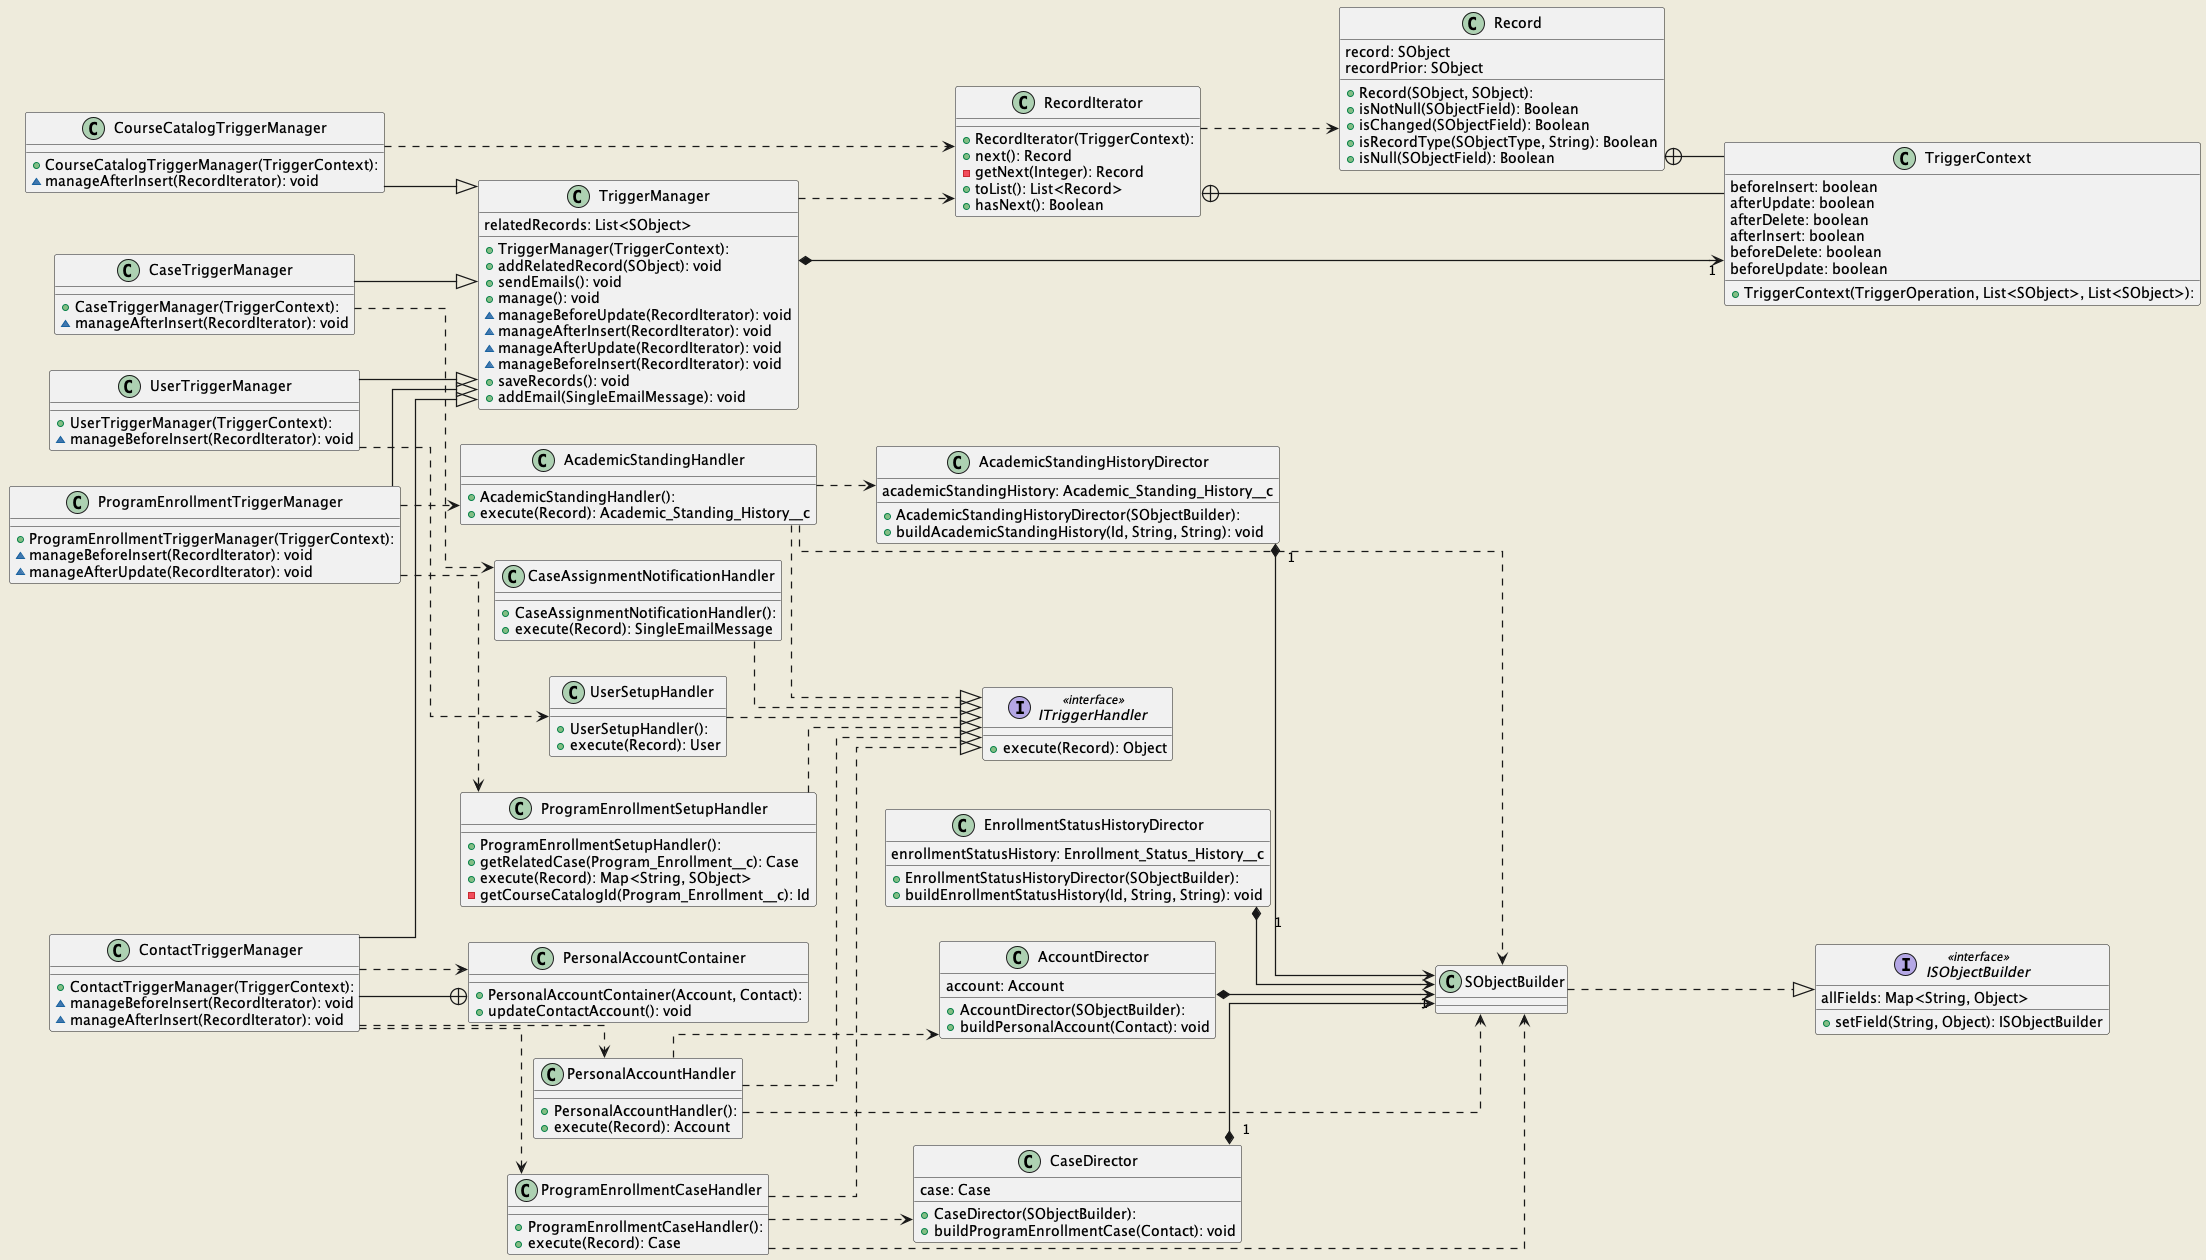
\includegraphics[
            width=\textwidth,
            height=8in
        ]{trigger-diagram}
        \caption{Trigger Subsystem}
        \label{fig:trigger-diagram}
    \end{figure}
    \newpage
    \begin{figure}[H]
        \centering
        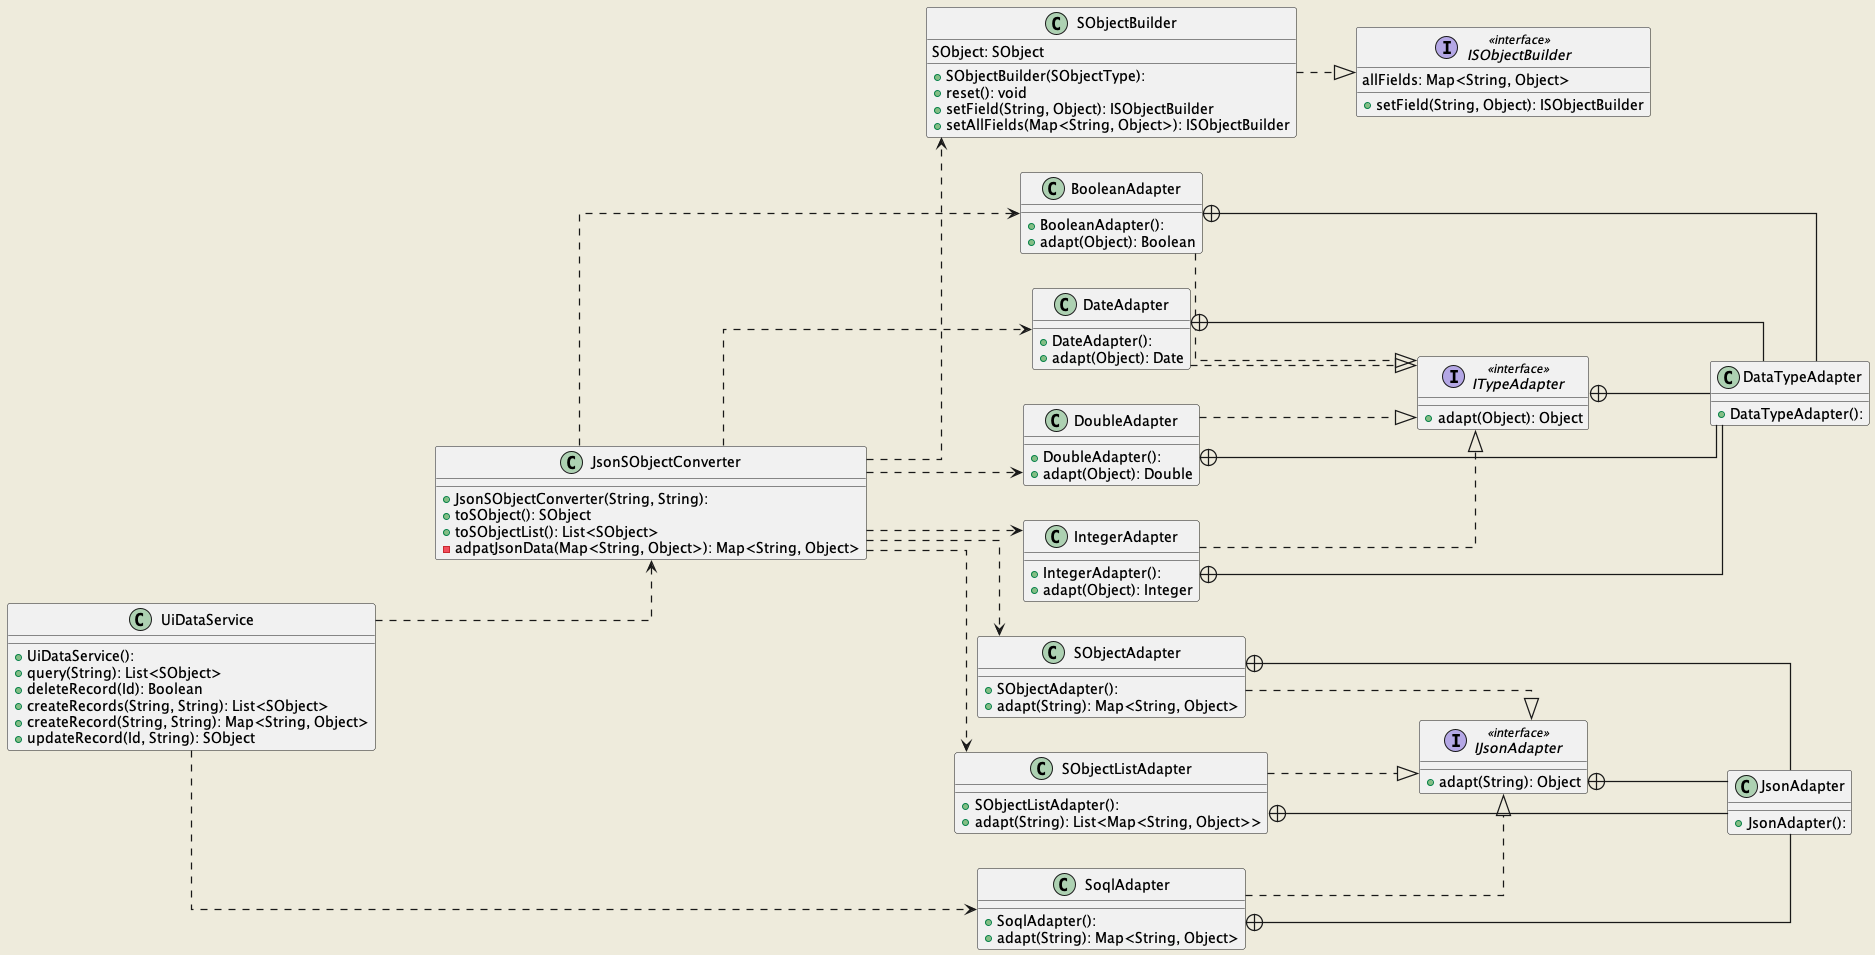
\includegraphics[
            width=1\textwidth,
            height=8.75in
        ]{service-diagram}
        \caption{Service Subsystem}
        \label{fig:service-diagram}
    \end{figure}

    \section{Screenshots of the Application}
    \begin{figure}[ht]
        \centering
        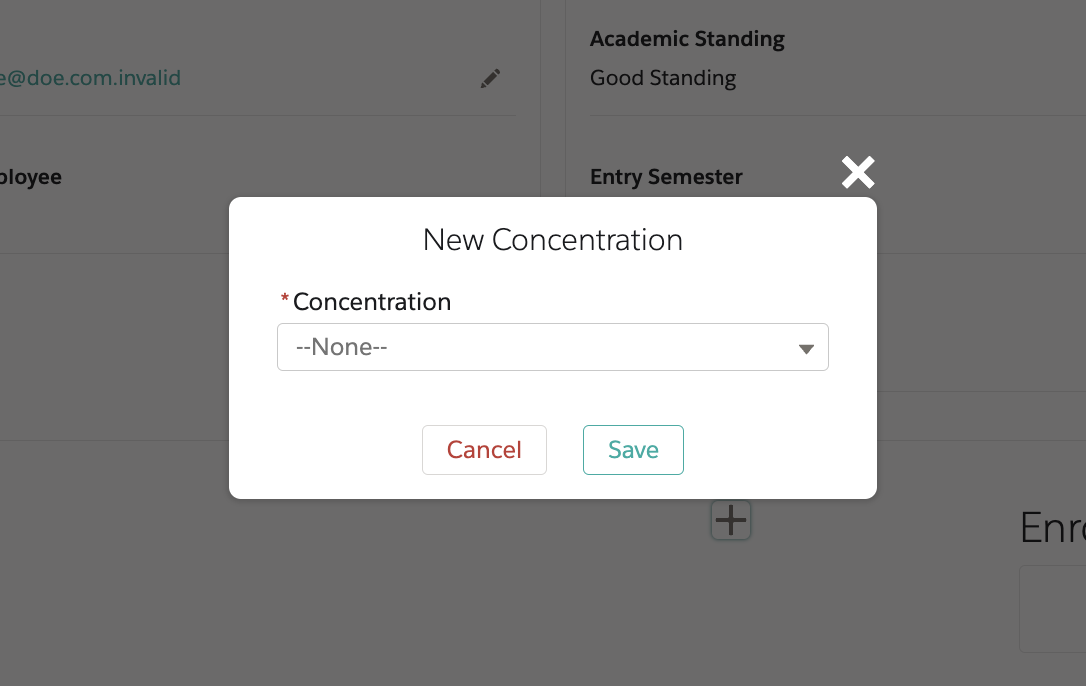
\includegraphics[max size={\textwidth}{\textheight}]{add-concentration-form}
        \label{fig:add-concentration-form}
        \caption{\textbf{Add Concentration Form}}
    \end{figure}
    
    \begin{figure}[ht]
        \centering
        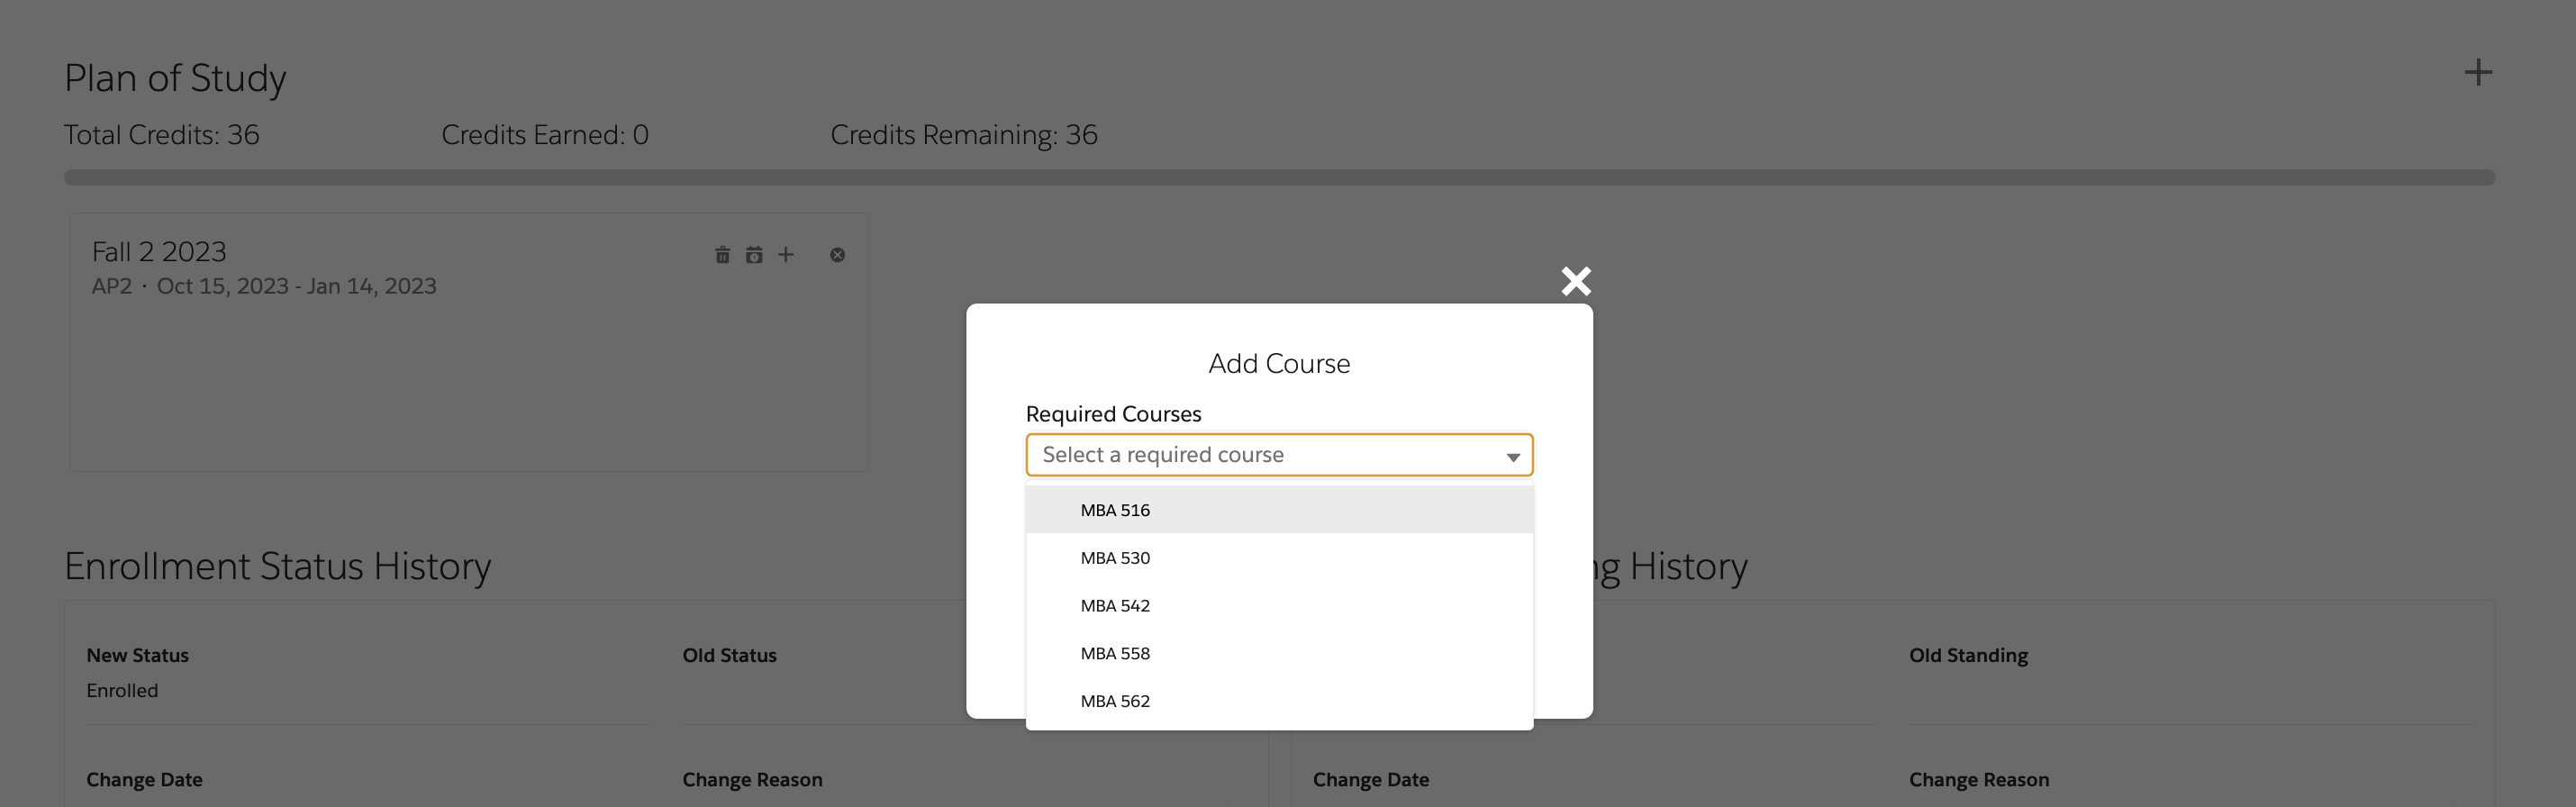
\includegraphics[max size={\textwidth}{\textheight}]{add-course-form}
        \label{fig:add-course-form}
        \caption{\textbf{Add Course Form}}
    \end{figure}
    
    \begin{figure}[ht]
        \centering
        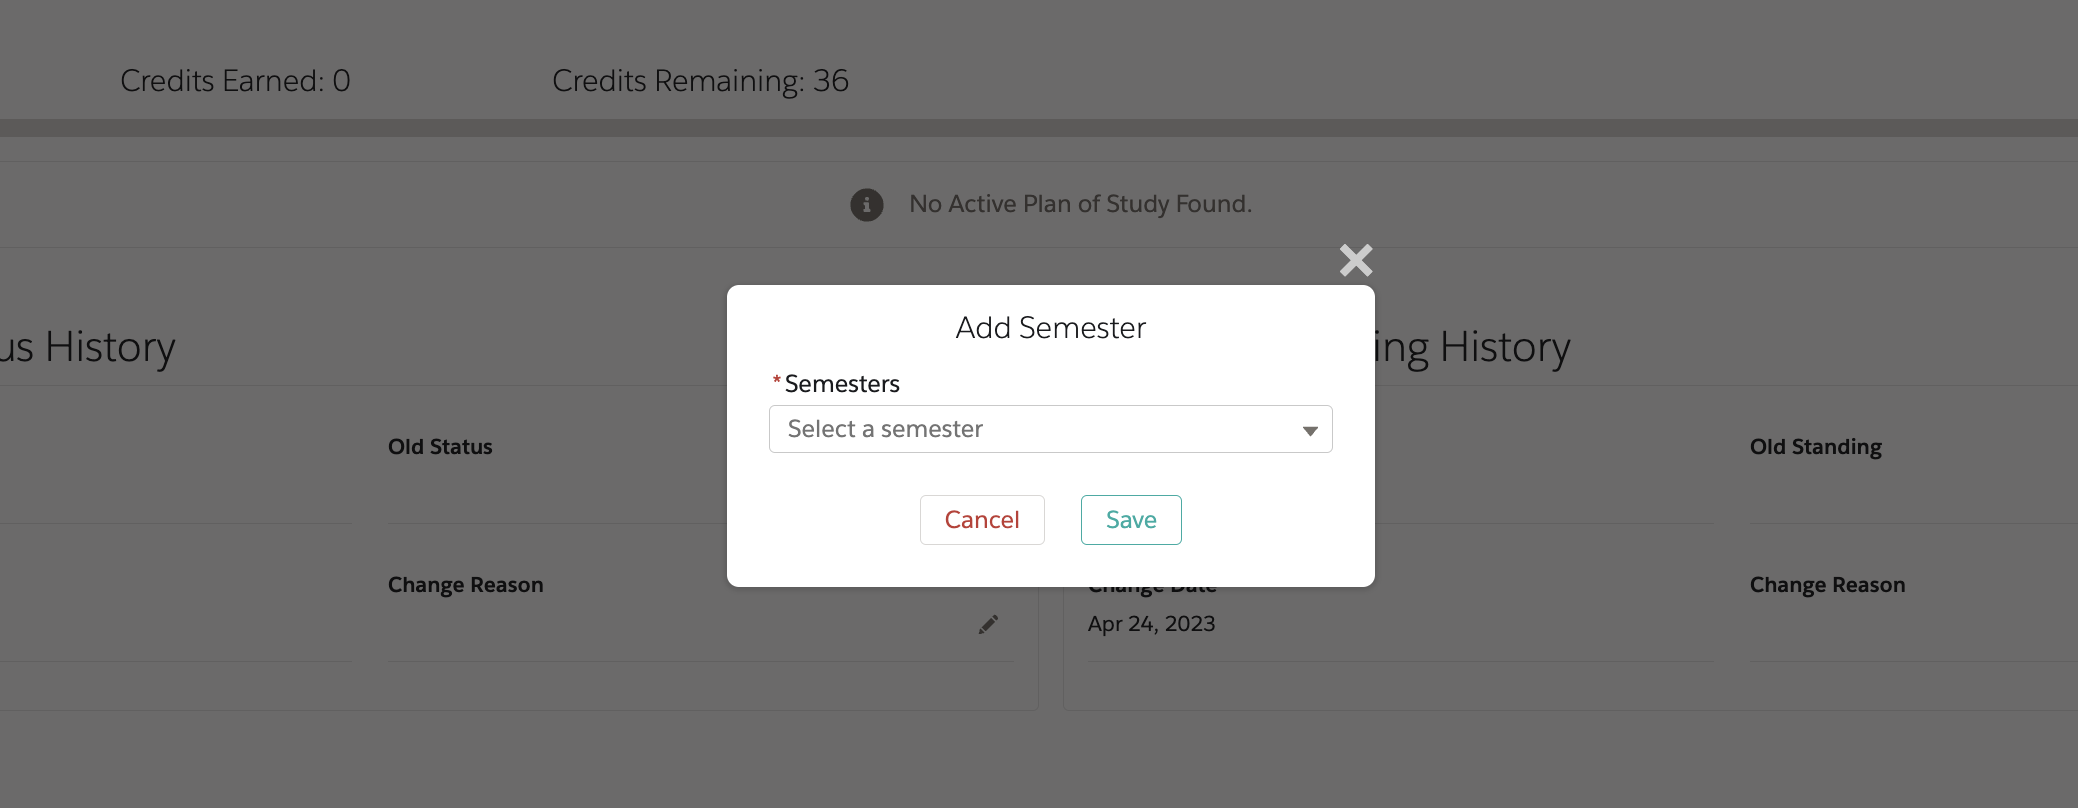
\includegraphics[max size={\textwidth}{\textheight}]{add-semester-form}
        \label{fig:add-semester-form}
        \caption{\textbf{Add Semester Form}}
    \end{figure}
    
    \begin{figure}[ht]
        \centering
        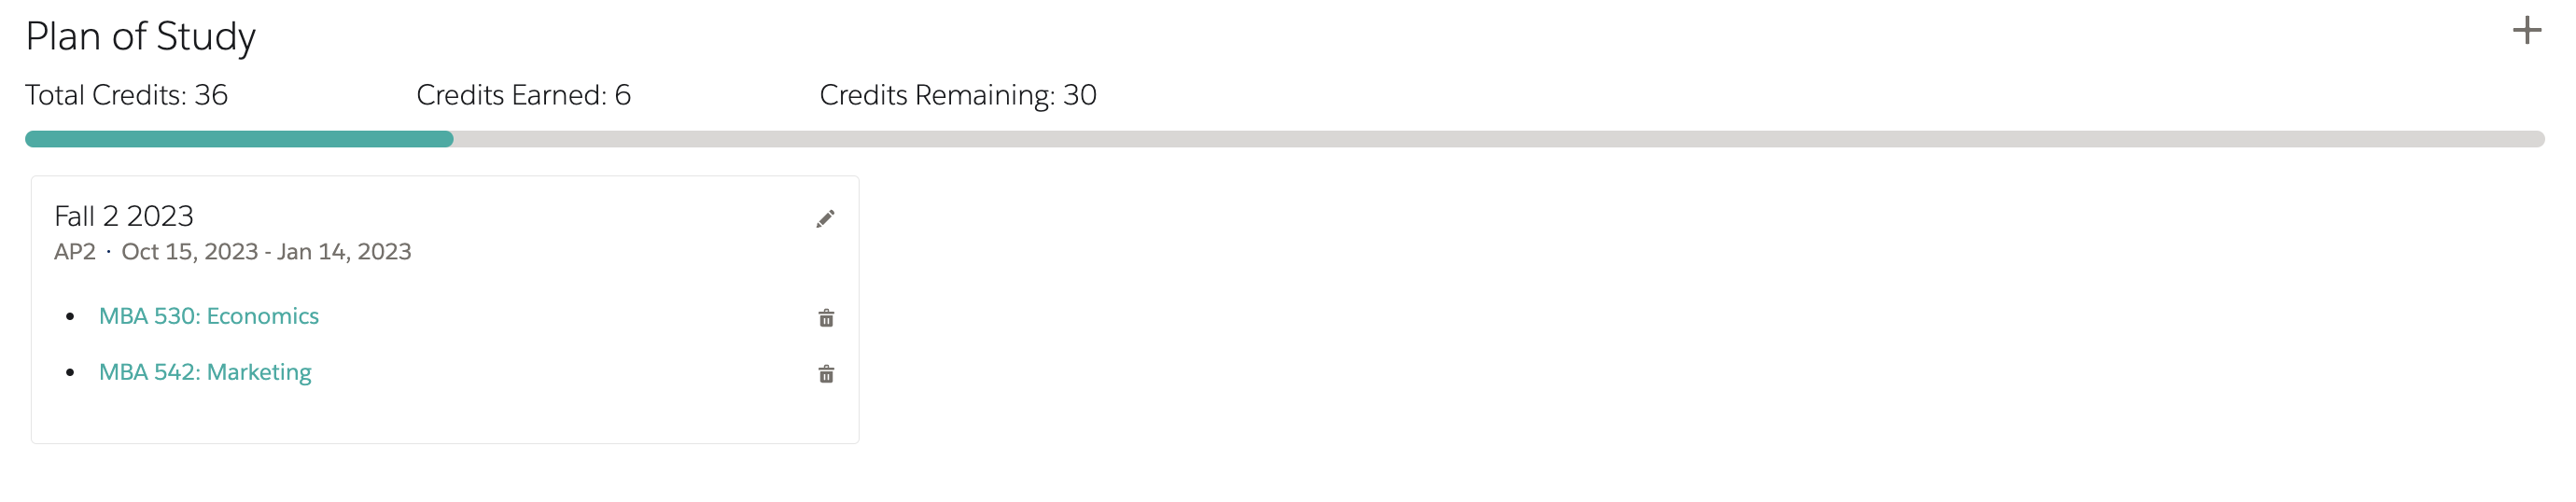
\includegraphics[max size={\textwidth}{\textheight}]{manage-plan-of-study}
        \label{fig:manage-plan-of-study}
        \caption{\textbf{Plan of Study View}}
    \end{figure}
    
    \begin{figure}[ht]
        \centering
        
\includegraphics[max size={\textwidth}{\textheight}]{remove-course-form}
        \label{fig:remove-course-form}
        \caption{\textbf{Remove Course Form}}
    \end{figure}
    
    \begin{figure}[ht]
        \centering
        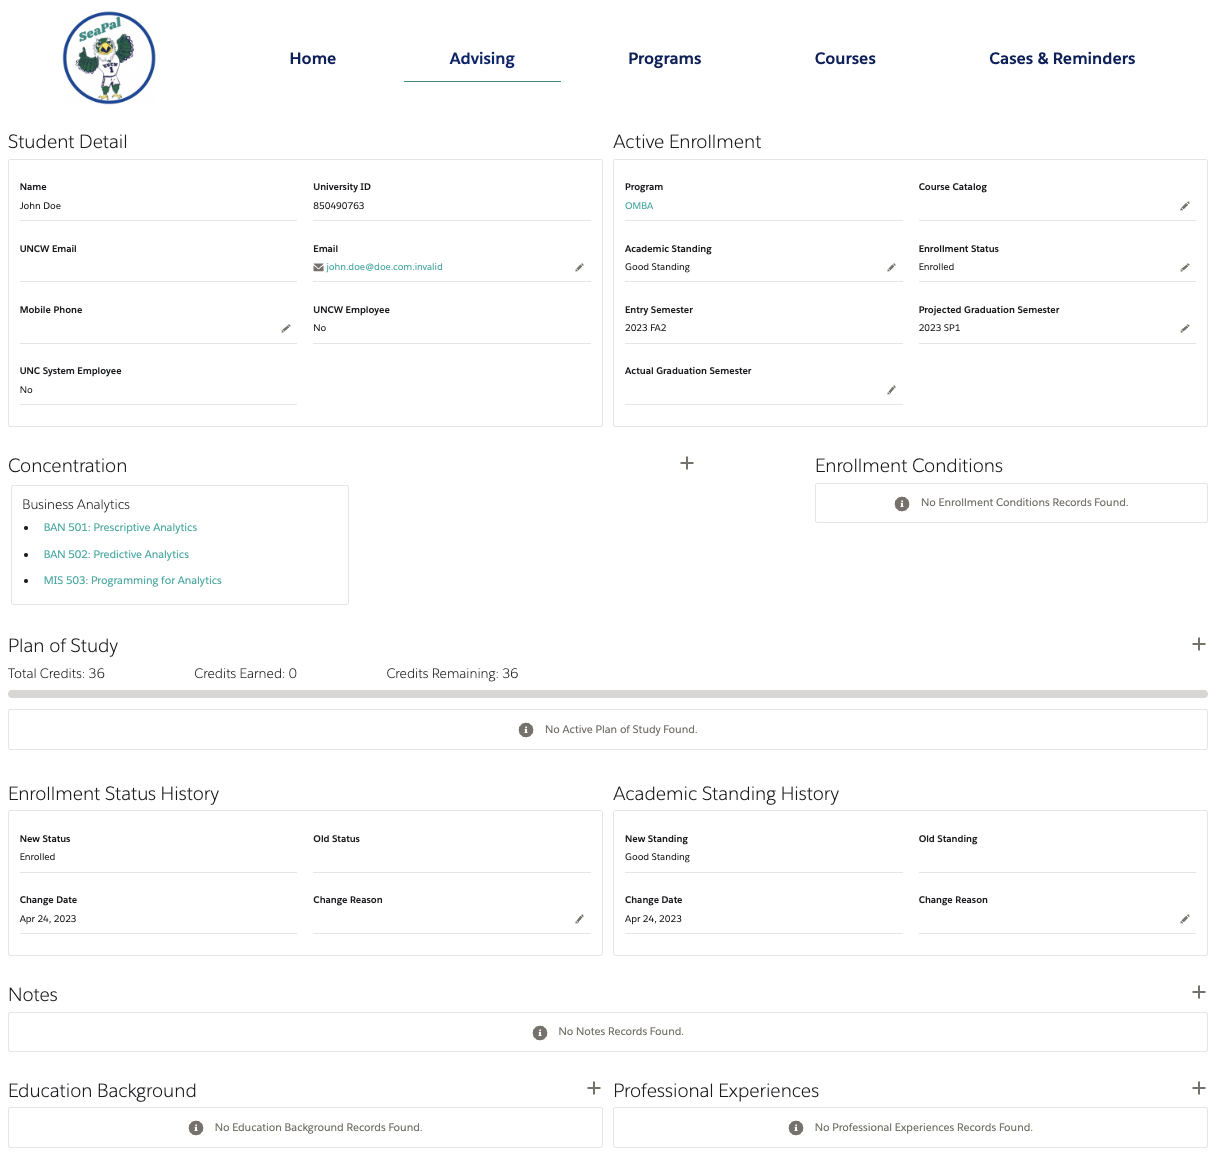
\includegraphics[max size={\textwidth}{\textheight}]{student-detail-page}
        \label{fig:student-detail-page}
        \caption{\textbf{Student Detail Page}}
    \end{figure}
    
    \begin{figure}[ht]
        \centering
        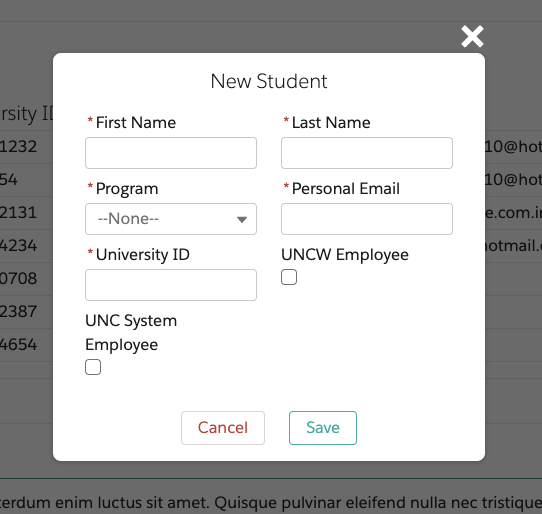
\includegraphics[max size={\textwidth}{\textheight}]{new-student-form}
        \label{fig:new-student-form}
        \caption{\textbf{New Student Form}}
    \end{figure}
    
    \begin{figure}[ht]
        \centering
        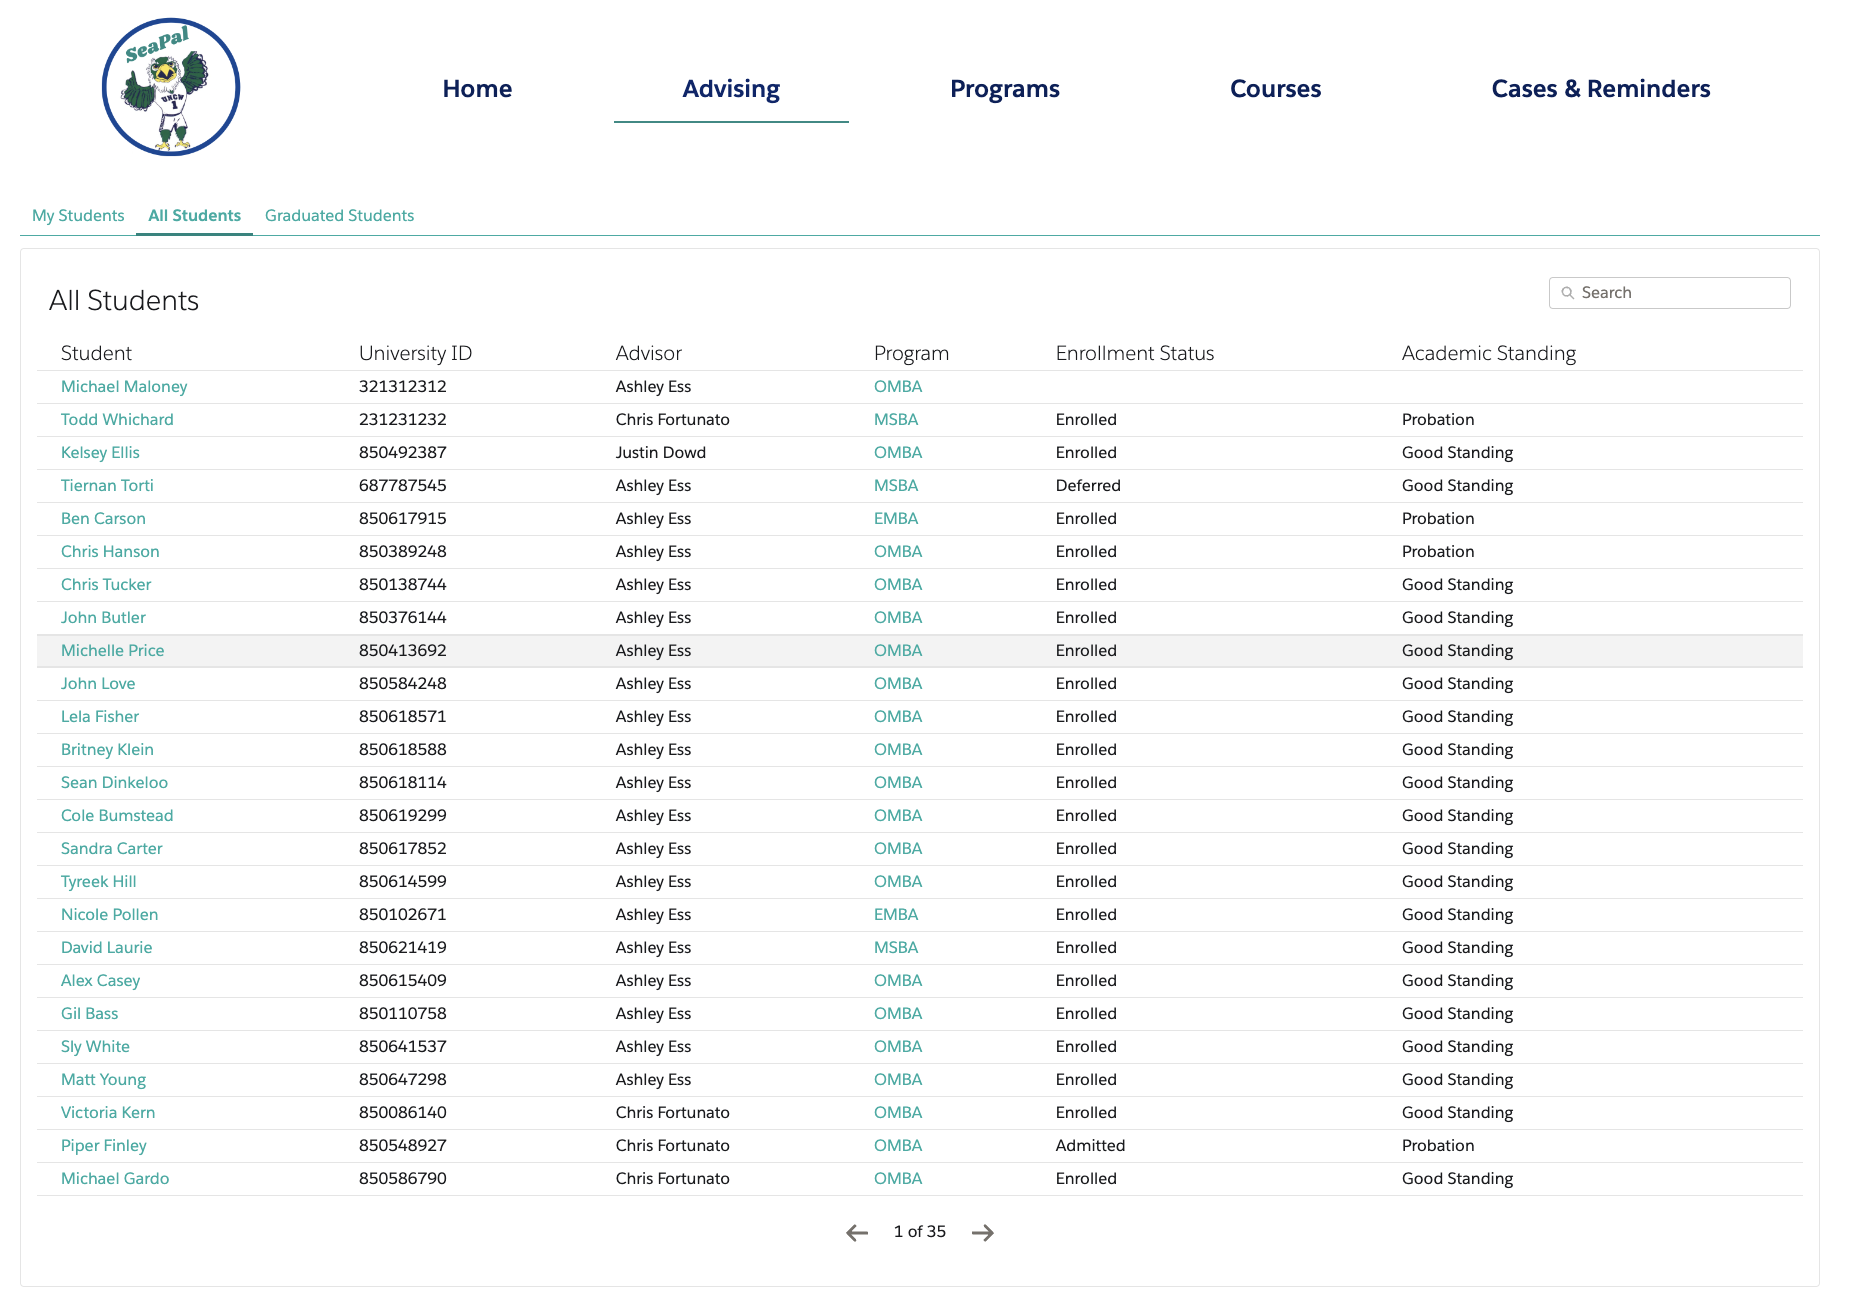
\includegraphics[max size={\textwidth}{\textheight}]{all-students-table}
        \label{fig:all-students-table}
        \caption{\textbf{Students Table}}
    \end{figure}
    
    \begin{figure}[ht]
        \centering
        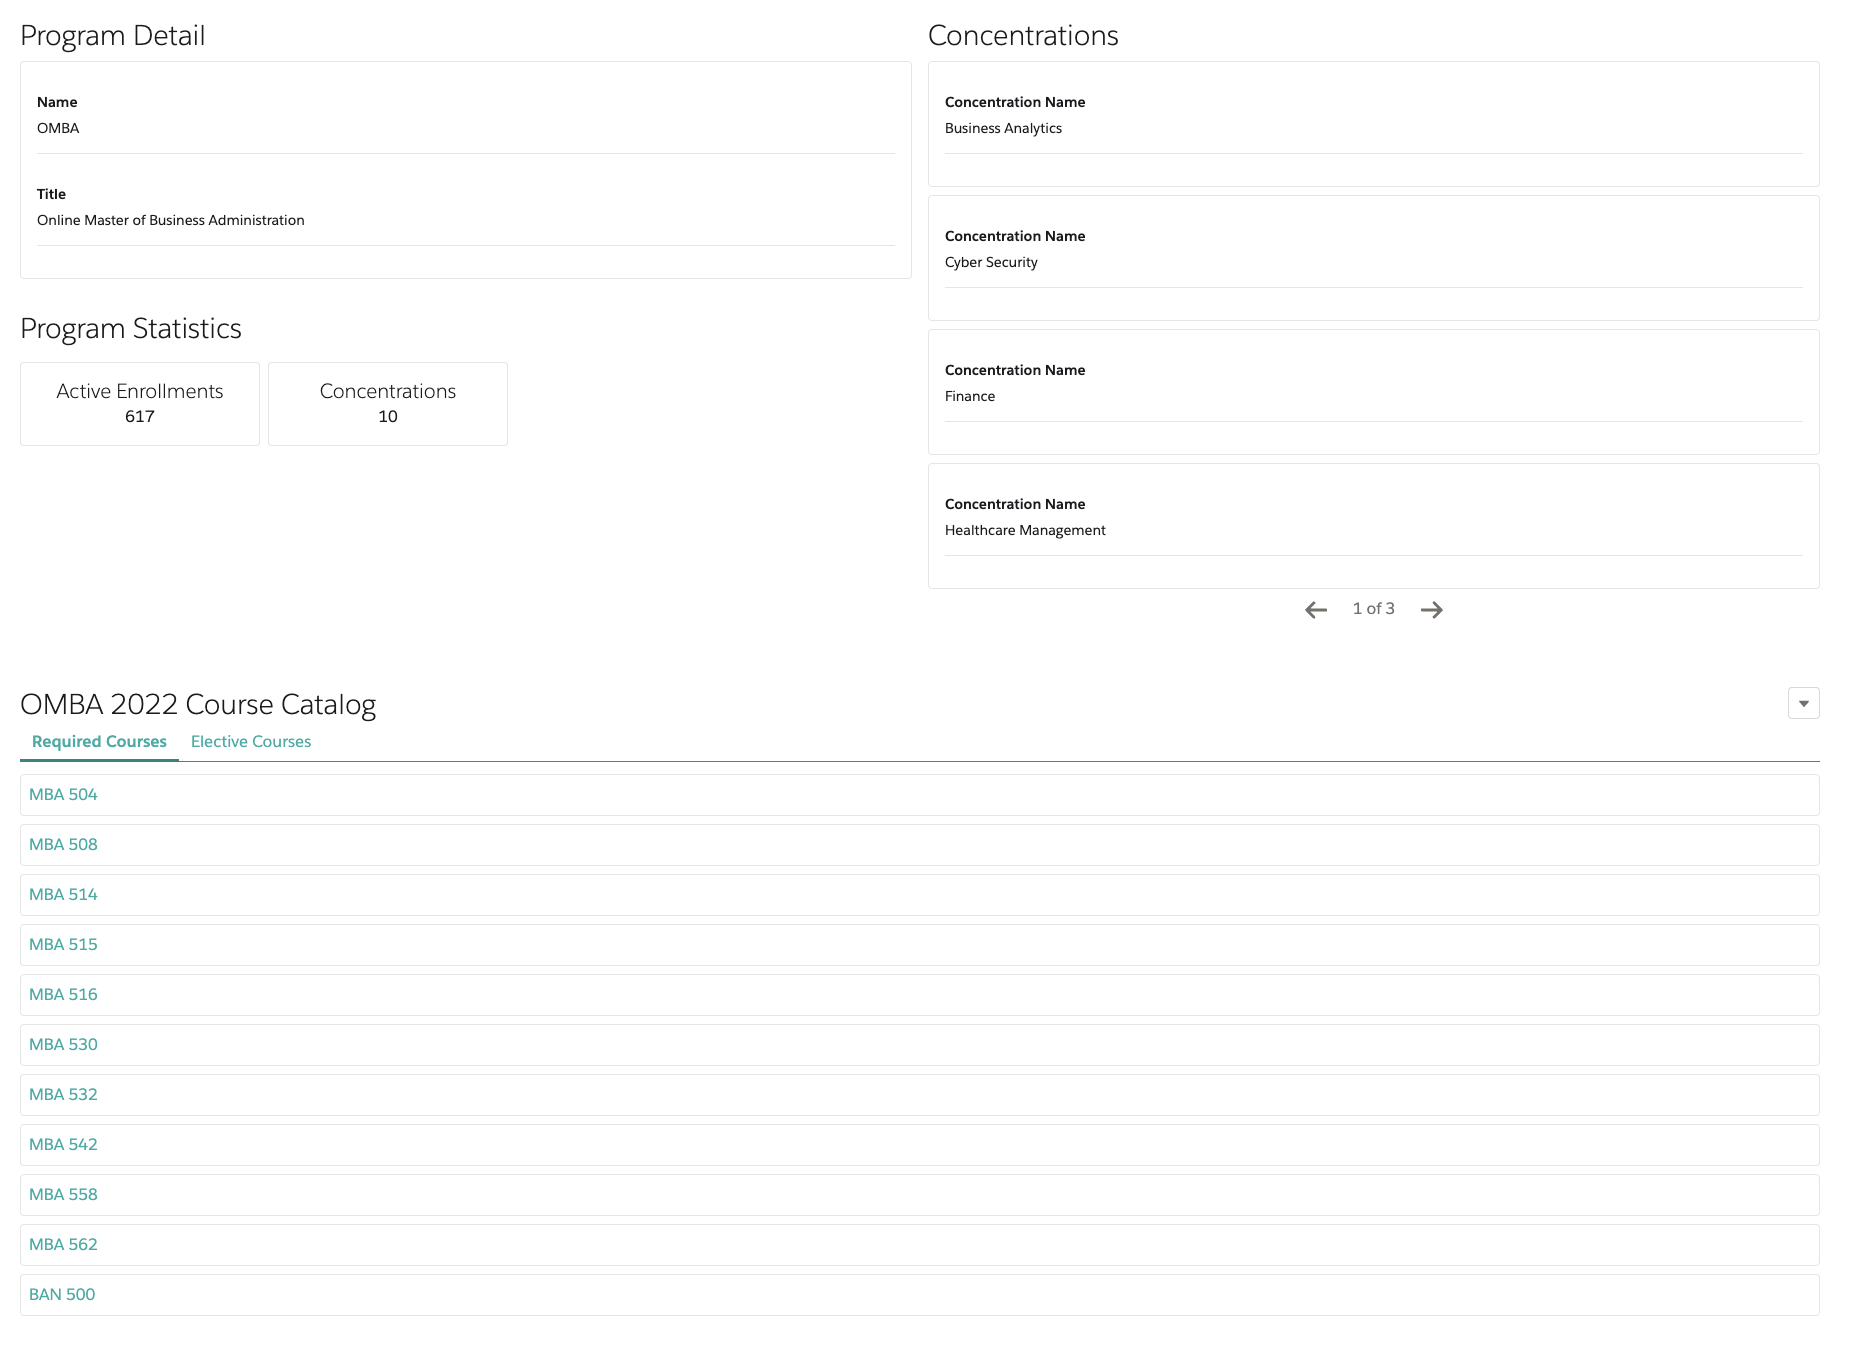
\includegraphics[max size={\textwidth}{\textheight}]{program-detail-page}
        \label{fig:program-detail-page}
        \caption{\textbf{Program Detail Page}}
    \end{figure}
\end{appendices}

\end{document}
